\documentclass[11pt,a4paper]{article}

% ── Packages ──
\usepackage[utf8]{inputenc}
\usepackage[T1]{fontenc}
\usepackage{fontspec}
\setmainfont{Liberation Sans}
\usepackage[margin=2.5cm]{geometry}
\usepackage{graphicx}
\usepackage{booktabs}
\usepackage{tabularx}
\usepackage{multirow}
\usepackage{caption}
\usepackage{subcaption}
\usepackage{hyperref}
\usepackage{xcolor}
\usepackage{amsmath,amssymb}
\usepackage[super,sort&compress]{natbib}
\usepackage{longtable}
\usepackage{array}
\usepackage{float}
\usepackage{enumitem}

\hypersetup{colorlinks=true, linkcolor=blue, citecolor=blue, urlcolor=blue}

% ── Title ──
\title{Population-referenced multi-omics analysis reveals mineral-pathway dysregulation in spaceflight: \\
       integrating NHANES baseline with astronaut and rodent transcriptomic data from the NASA OSDR}
\author{Richard Barker}
\date{}

\begin{document}

\maketitle

% ════════════════════════════════════════════════════════════════════
% ABSTRACT
% ════════════════════════════════════════════════════════════════════
\begin{abstract}
\noindent
Spaceflight disrupts mineral homeostasis through microgravity-induced bone loss, fluid shifts, and radiation exposure, yet interpreting clinical markers from small astronaut cohorts ($n=4$) lacks population context. We integrated data from the National Health and Nutrition Examination Survey (NHANES, 2013--2018, $n=5{,}748$ adults aged 40--60) as a population reference baseline for 15 clinical mineral and hematological variables, then contextualized measurements from four Inspiration4 astronauts across seven timepoints. We further extended the NHANES reference with four iron status markers (serum iron, ferritin, transferrin saturation, TIBC) not measured in astronauts, establishing population correlations between iron status and CBC parameters (hemoglobin vs.\ serum iron $r = 0.424$, vs.\ transferrin saturation $r = 0.412$). Mean platelet volume was significantly elevated above population norms at six of seven timepoints (Benjamini--Hochberg FDR $< 0.05$, Cohen's $d = 2.12$--$2.47$), while calcium ($d = 1.30$--$1.92$) and bicarbonate ($d = -1.24$ to $-1.78$) showed large population-deviating effects. Transcriptomic analysis identified 50 differentially expressed mineral-pathway genes, with copper-dependent enzymes (APP up, LOX/LOXL1 down), iron metabolism genes (ALAS2 down, HFE up), and the calcium channel CACNA1D (down, log$_2$FC $= -2.25$) most affected. Machine learning regression demonstrated that mineral-pathway gene expression predicts serum potassium ($r = 0.50$) and sodium ($r = 0.46$) under leave-one-out cross-validation. A cross-species meta-analysis across 28 rodent datasets revealed significant mineral-pathway concordance in skeletal muscle (pooled $r = 0.035$, $p = 0.0025$), strongest in soleus ($r = 0.059$, $p = 0.009$), but not in liver or kidney. These findings demonstrate that population-referenced framing reveals spaceflight mineral deviations invisible to within-subject analysis alone, with implications for biomarker development and nutritional countermeasures.

\medskip
\noindent\textbf{Keywords:} spaceflight, mineral homeostasis, NHANES, multi-omics, transcriptomics, cross-species meta-analysis, machine learning, Inspiration4, NASA OSDR
\end{abstract}

% ════════════════════════════════════════════════════════════════════
% INTRODUCTION
% ════════════════════════════════════════════════════════════════════
\section{Introduction}

Spaceflight exposes humans to a unique combination of physiological stressors including microgravity, cosmic radiation, confinement, and altered circadian rhythms. These stressors disrupt multiple biological systems\textsuperscript{1}, with mineral homeostasis being particularly vulnerable: microgravity-induced bone resorption releases calcium into the circulation\textsuperscript{11}, cephalad fluid shifts expand central blood volume\textsuperscript{2}, and spaceflight increases oxidative stress\textsuperscript{3}. The NASA Open Science Data Repository (OSDR) provides multi-omics data from the Inspiration4 (I4) mission --- the first all-civilian orbital spaceflight (September 2021, 3-day low-Earth orbit)\textsuperscript{4} --- including RNA-seq, proteomics, metabolomics, and clinical chemistry from four astronauts across seven timepoints.

A fundamental challenge in spaceflight omics research is the extremely small sample size. With $n=4$ astronauts, within-subject comparisons lack the statistical power to distinguish spaceflight-induced changes from normal biological variation. Population reference data can address this limitation by providing an external baseline against which astronaut values can be compared. The National Health and Nutrition Examination Survey (NHANES), conducted by the CDC National Center for Health Statistics, provides nationally representative laboratory data for the U.S. civilian population\textsuperscript{5}, including standard biochemistry profiles and complete blood counts that directly overlap with astronaut clinical measurements.

In this study, we: (1) established NHANES population reference intervals for 15 clinical mineral and hematological variables matched to astronaut data; (2) extended the NHANES reference with four iron status markers (serum iron, ferritin, transferrin saturation, TIBC) not measured in astronauts, and quantified population-level correlations between iron status and CBC parameters; (3) identified astronaut markers that deviate significantly from population norms; (4) characterized the mineral-pathway transcriptomic response using curated gene sets spanning 10 minerals and 5 KEGG pathways; (5) evaluated whether mineral-pathway gene expression predicts serum mineral levels using machine learning; (6) integrated per-sample RNA-seq from two independent missions (I4, $n = 4$; AX-1, $n = 2$) via a denoising autoencoder with leave-one-astronaut-out cross-validation; (7) validated the mineral-pathway signature against the independent JAXA6 mission ($n = 6$ astronauts); and (8) conducted a cross-species meta-analysis across 28 rodent datasets to assess translational concordance. By framing astronaut findings within a population baseline and validating across missions and species, we distinguish population-deviating abnormalities from within-subject variation that may remain within normal physiological ranges.

% ════════════════════════════════════════════════════════════════════
% RESULTS
% ════════════════════════════════════════════════════════════════════
\section{Results}

\subsection{NHANES population reference for clinical mineral markers}

We pooled three consecutive NHANES cycles (2013--2014, 2015--2016, 2017--2018) to construct a stable population reference for 15 clinical variables that directly map to astronaut measurements: five biochemistry analytes (calcium, potassium, sodium, chloride, bicarbonate) from the Standard Biochemistry Profile and ten hematological parameters (hemoglobin, hematocrit, RBC count, MCH, MCHC, MCV, WBC count, RDW, platelet count, MPV) from the Complete Blood Count with 5-part differential. The reference population was restricted to adults aged 40--60 years (all sexes), yielding 5,748 participants (2,713 male, 3,035 female) --- demographically consistent with typical astronaut corps age ranges. Reference intervals (P2.5--P97.5), means, standard deviations, and full percentile distributions were computed for each variable (Table~\ref{tab:nhanes_ref}).

\begin{table}[H]
\centering
\caption{NHANES population reference statistics for key clinical mineral and hematological variables (age 40--60, all sexes, pooled 2013--2018).}
\label{tab:nhanes_ref}
\begin{tabular}{lrlrrr}
\toprule
\textbf{Variable} & \textbf{N} & \textbf{Units} & \textbf{Mean} & \textbf{P2.5} & \textbf{P97.5} \\
\midrule
Calcium & 5,429 & mg/dL & 9.33 & 8.70 & 10.00 \\
Potassium & 5,442 & mmol/L & 3.98 & 3.30 & 4.70 \\
Sodium & 5,444 & mmol/L & 139.48 & 135.00 & 144.00 \\
Chloride & 5,444 & mmol/L & 102.83 & 96.00 & 108.00 \\
Bicarbonate & 5,444 & mmol/L & 25.13 & 21.00 & 30.00 \\
Hemoglobin & 5,519 & g/dL & 14.08 & 10.70 & 16.70 \\
Hematocrit & 5,519 & \% & 41.92 & 33.09 & 49.60 \\
RBC count & 5,519 & M/uL & 4.73 & 3.84 & 5.71 \\
MCH & 5,519 & pg & 29.07 & 22.80 & 33.30 \\
MCHC & 5,519 & g/dL & 33.50 & 31.40 & 35.10 \\
MCV & 5,519 & fL & 88.38 & 70.69 & 98.70 \\
WBC count & 5,519 & 10$^3$/uL & 7.28 & 3.90 & 12.21 \\
RDW & 5,519 & \% & 13.84 & 12.30 & 17.61 \\
Platelet count & 5,519 & 10$^3$/uL & 243.54 & 140.00 & 383.00 \\
MPV & 5,519 & fL & 8.36 & 6.80 & 10.40 \\
\bottomrule
\end{tabular}
\end{table}

\subsection{Astronaut clinical markers deviate from population norms}

Each of the 28 astronaut measurements (4 crew $\times$ 7 timepoints) was converted to a z-score relative to the NHANES age 40--60 reference and evaluated for deviation from the population 95\% reference interval (P2.5--P97.5). One-sample $t$-tests and Wilcoxon signed-rank tests were performed at each timepoint, with Benjamini--Hochberg FDR correction across all 105 tests (15 variables $\times$ 7 timepoints). Three implausible values in one crew member (C003 at L-92: MPV = 330 fL, RDW = 32.4\%, platelet count = 12.9 $\times$ 10$^3$/uL) were identified as data entry errors and excluded.

Mean platelet volume (MPV) was significantly elevated above the NHANES population mean at six of seven timepoints (FDR $< 0.05$; Cohen's $d$ ranging from 2.12 to 2.47); at L-92, where only three crew were measured, the elevation was smaller and not significant after correction ($d = 1.73$, FDR $= 0.13$), with 48.1\% of astronaut MPV measurements falling outside the population 95\% reference interval (Figure~\ref{fig:zscore_heatmap}). This deviation was persistent across pre-flight, flight, and post-flight phases, suggesting a crew-level characteristic rather than a spaceflight-induced shift.

\begin{figure}[H]
\centering
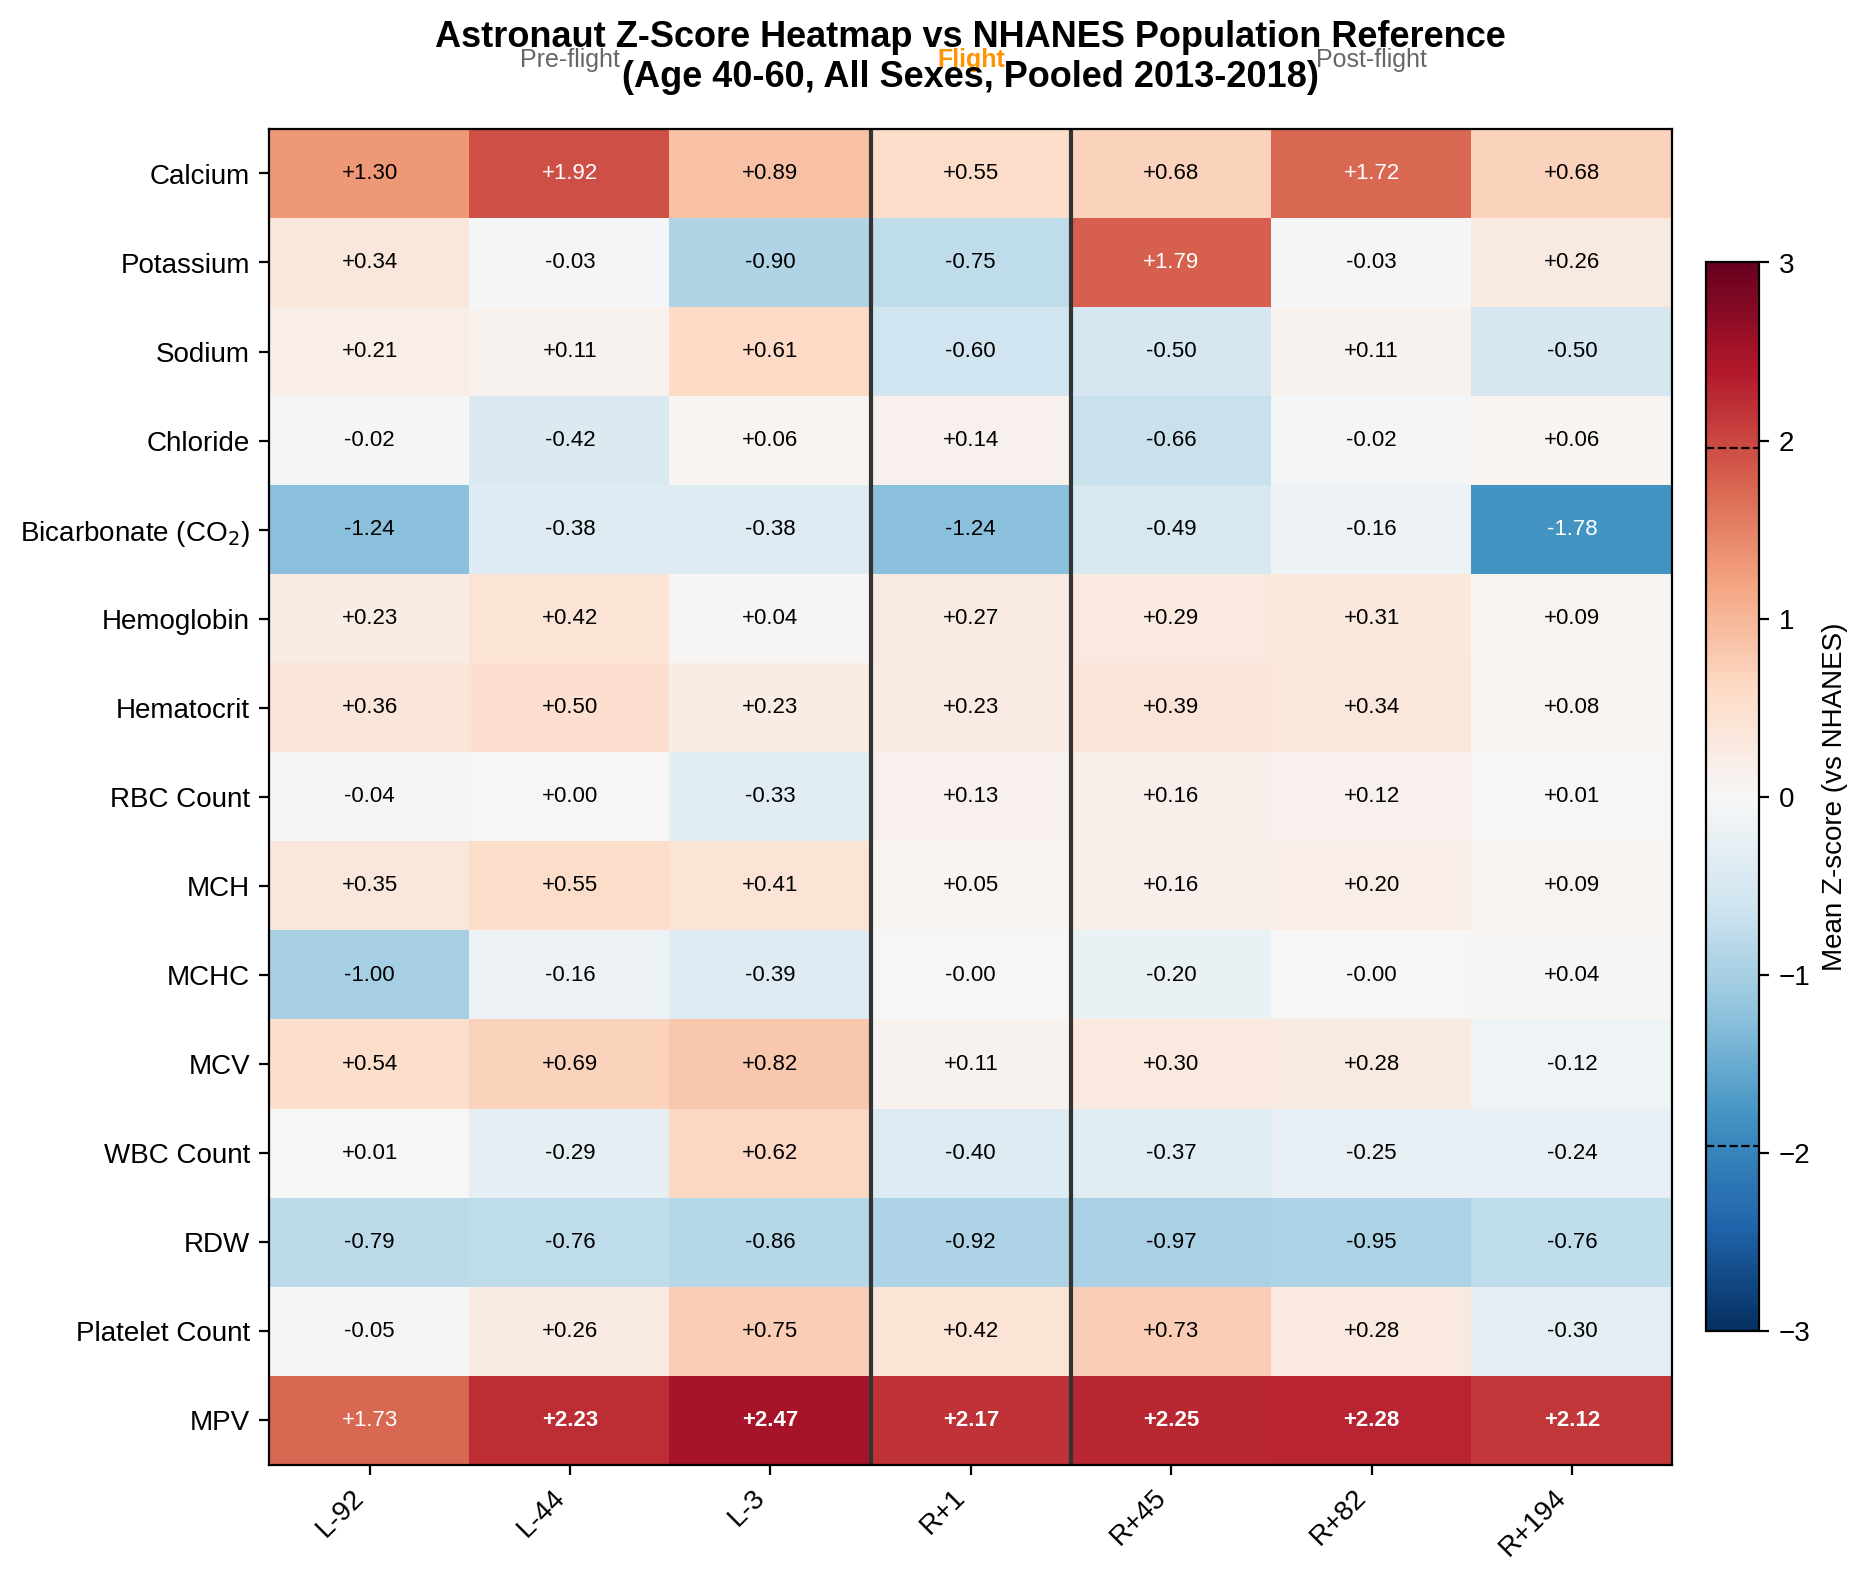
\includegraphics[width=0.85\textwidth]{figures/fig_s7_zscore_heatmap.png}
\caption{Astronaut z-score heatmap against NHANES population reference (age 40--60, all sexes, pooled 2013--2018). Cell values represent mean astronaut z-scores for each variable at each timepoint. Bold text indicates $|z| \geq 1.96$ (population-significant deviation). Diverging colormap centered at zero (blue = below population mean, red = above). Vertical lines separate pre-flight (L-92, L-44, L-3), flight (R+1), and post-flight (R+45, R+82, R+194) phases.}
\label{fig:zscore_heatmap}
\end{figure}

Calcium showed large positive effect sizes at multiple timepoints (Cohen's $d = 1.30$ at L-92, $d = 1.92$ at L-44, $d = 1.72$ at R+82), with 17.9\% of measurements outside the reference interval. Notably, calcium z-scores were elevated even at pre-flight baseline (L-92: $d = 1.30$; L-44: $d = 1.92$), indicating that this population deviation pre-dates spaceflight exposure. Bicarbonate (CO$_2$) was consistently below the population mean ($d = -1.24$ at L-92 and R+1; $d = -1.78$ at R+194), with 14.3\% of measurements outside the lower reference bound. RDW was consistently below the population mean ($d = -0.86$ to $-0.97$), with 18.5\% of measurements outside the lower reference bound.

In contrast, sodium, chloride, MCH, MCV, and WBC count remained within the population reference range across all timepoints (0\% outside P2.5--P97.5), indicating these electrolytes and erythrocyte indices are robust to spaceflight-related perturbation at the group level. Hemoglobin, hematocrit, and RBC count showed modest deviations (3.7--7.4\% outside reference) with small effect sizes, consistent with the known mild spaceflight-associated anemia pattern\textsuperscript{6}.

\begin{figure}[H]
\centering
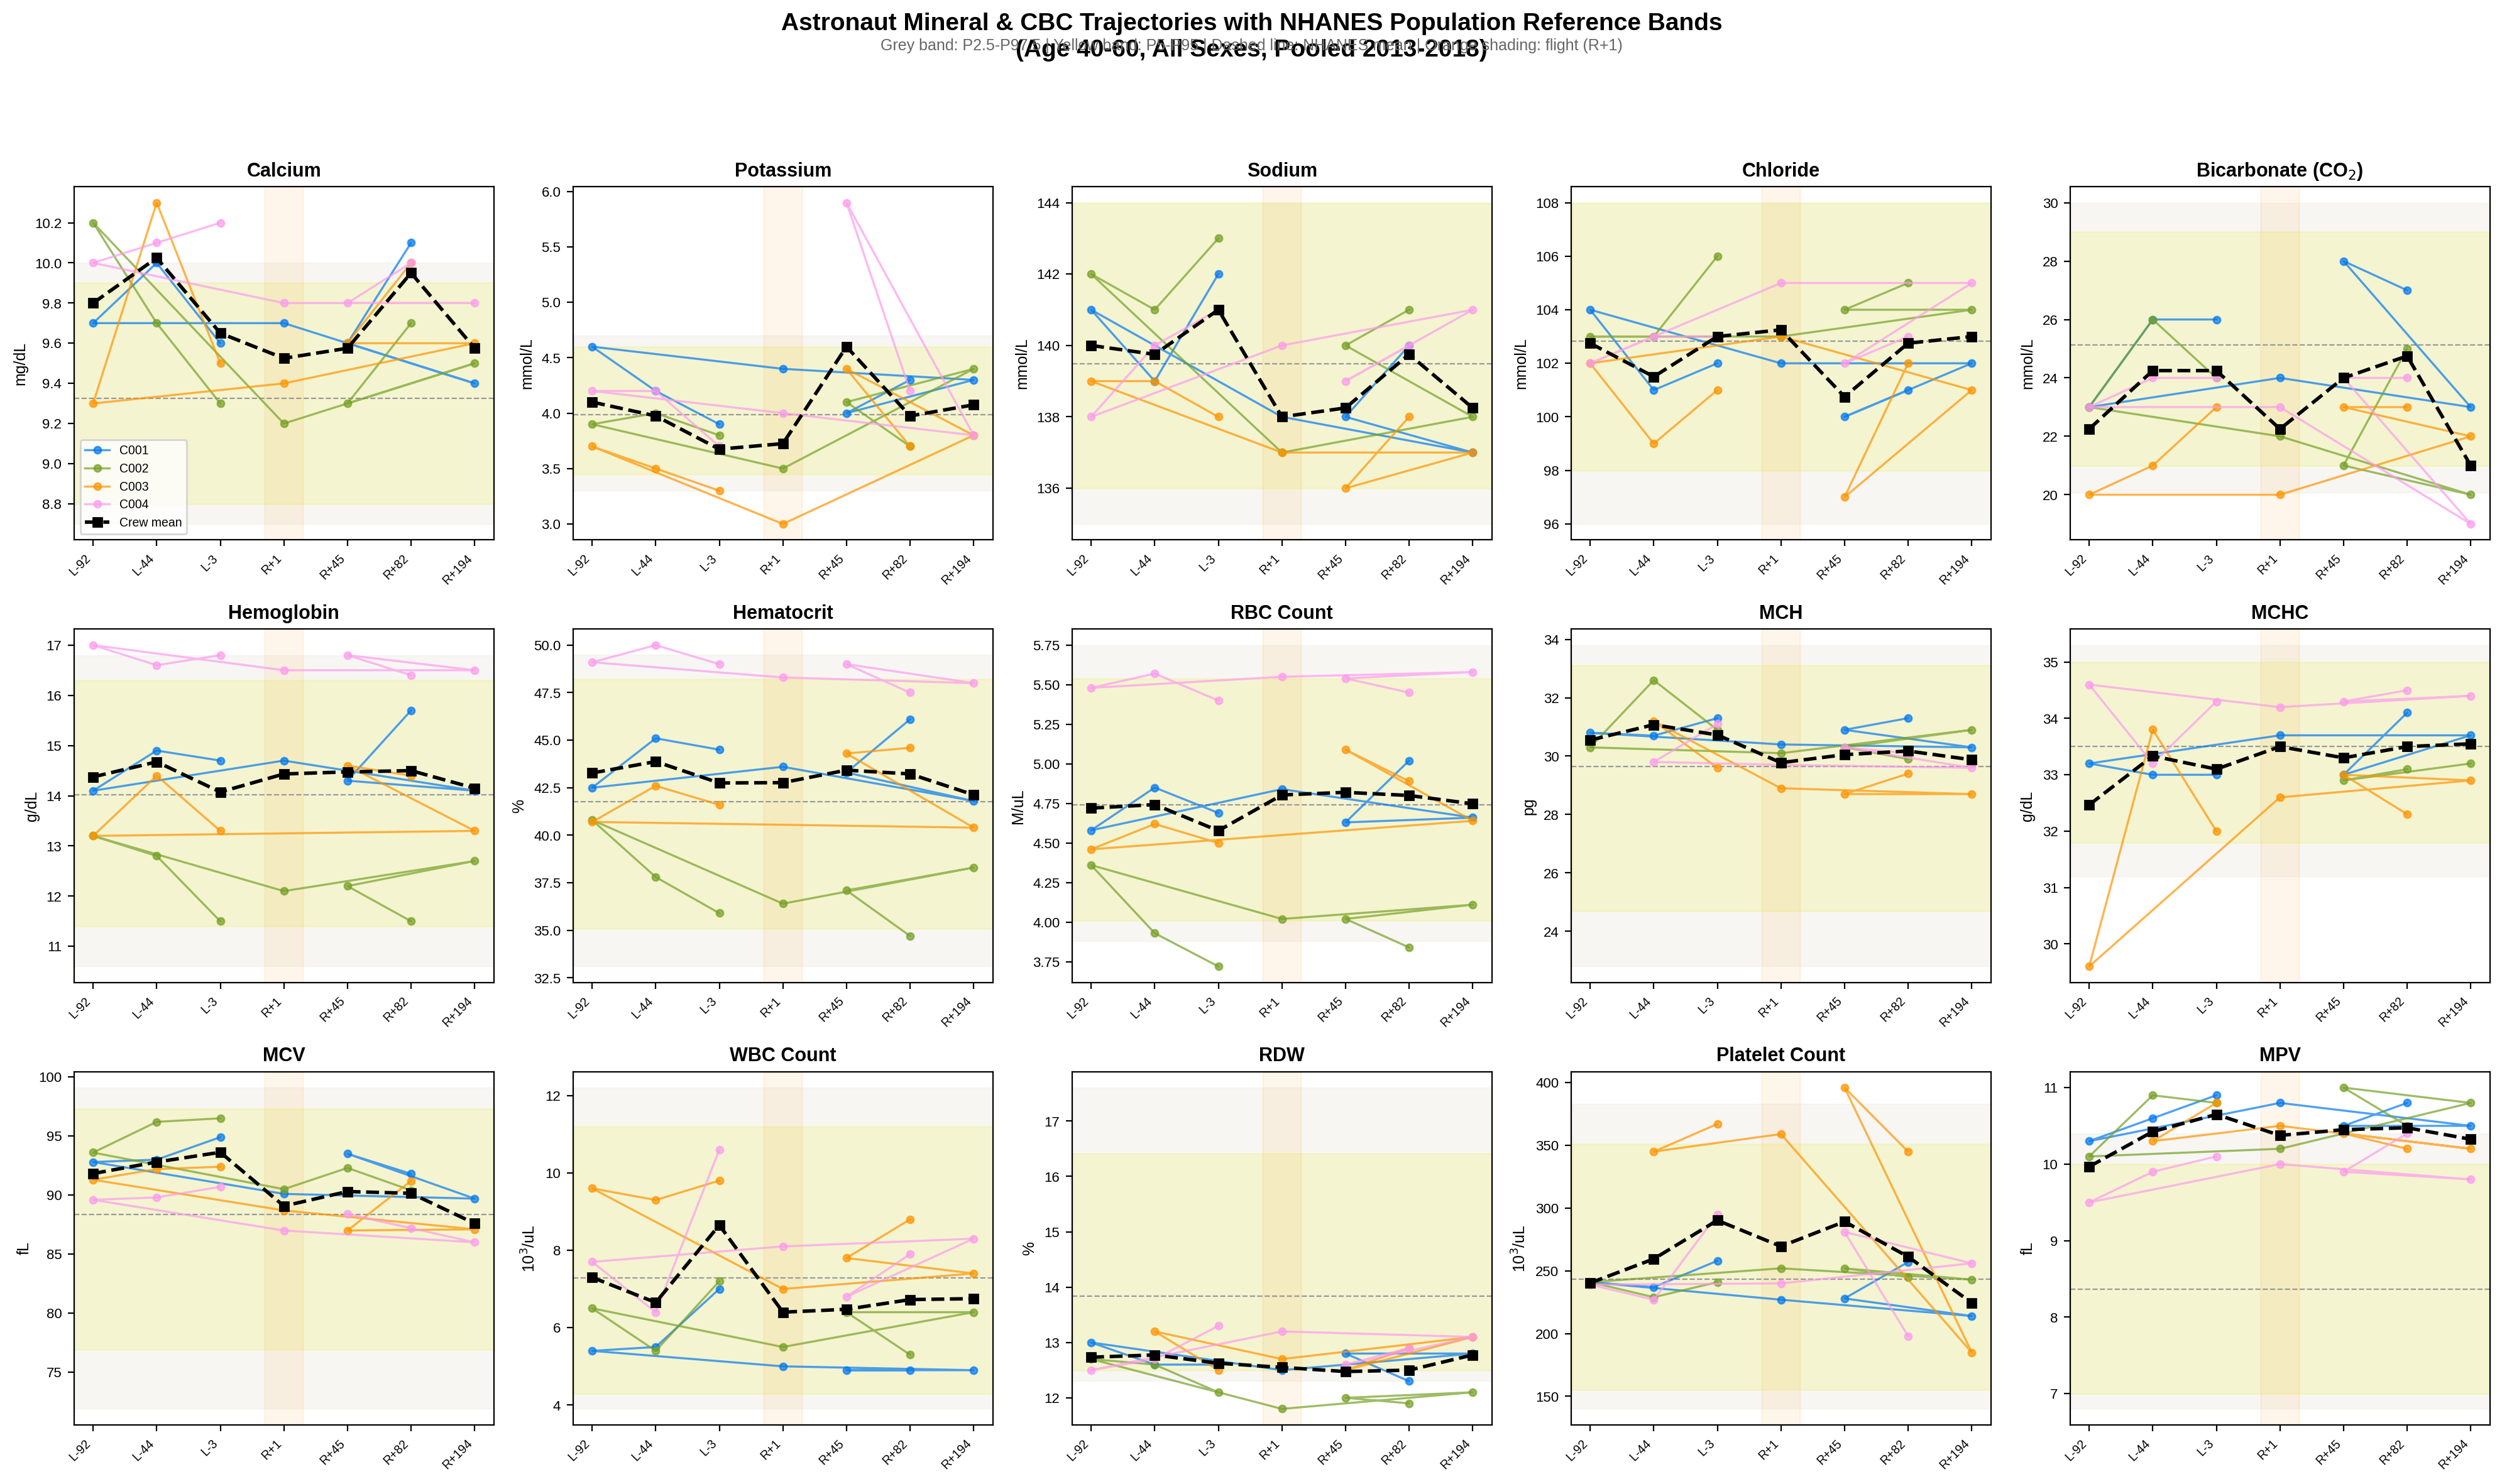
\includegraphics[width=\textwidth]{figures/fig_s6_nhanes_trajectories.png}
\caption{Astronaut mineral and CBC trajectories with NHANES population reference bands. Each panel shows one variable across seven timepoints (L-92 through R+194). Grey band: NHANES P2.5--P97.5 reference interval; yellow band: P5--P95; dashed line: NHANES mean. Colored lines: four individual astronauts; black squares: crew mean. Orange shading marks the flight timepoint (R+1). Reference population: age 40--60, all sexes, pooled NHANES 2013--2018 ($n = 5{,}748$).}
\label{fig:trajectories}
\end{figure}

The trajectory plots (Figure~\ref{fig:trajectories}) reveal that several population-deviating markers (calcium, MPV, bicarbonate) show deviations at pre-flight baseline, while others (potassium at R+45, $d = 1.79$) show transient spaceflight-associated shifts. Percentile ranks for all measurements are shown in Supplementary Figure~S1, and full one-sample test results are provided in Table~\ref{tab:onesample}.

\begin{table}[H]
\centering
\caption{One-sample test results for astronaut markers with large population deviations. Cohen's $d$ computed using NHANES pooled SD. FDR: Benjamini--Hochberg adjusted $p$-value across 105 tests.}
\label{tab:onesample}
\begin{tabular}{llrrrr}
\toprule
\textbf{Variable} & \textbf{Timepoint} & \textbf{Cohen's $d$} & \textbf{$t$ $p$-value} & \textbf{FDR} & \textbf{\% outside ref} \\
\midrule
\multicolumn{6}{l}{\textit{FDR-significant ($< 0.05$)}} \\
MPV & L-3 & 2.47 & 0.001 & 0.048 & 75.0 \\
MPV & R+82 & 2.28 & 0.0005 & 0.047 & 50.0 \\
MPV & L-44 & 2.23 & 0.002 & 0.048 & 50.0 \\
MPV & R+45 & 2.25 & 0.003 & 0.048 & 50.0 \\
MPV & R+1 & 2.17 & 0.001 & 0.048 & 50.0 \\
MPV & R+194 & 2.12 & 0.003 & 0.048 & 50.0 \\
\midrule
\multicolumn{6}{l}{\textit{Large effect ($|d| \geq 0.8$), not FDR-significant}} \\
Calcium & L-44 & 1.92 & 0.011 & 0.115 & 50.0 \\
Potassium & R+45 & 1.79 & 0.257 & 0.649 & 25.0 \\
Bicarbonate & R+194 & $-1.78$ & 0.020 & 0.135 & 25.0 \\
MPV & L-92 & 1.73 & 0.022 & 0.135 & 50.0 \\
Calcium & R+82 & 1.72 & 0.006 & 0.065 & 25.0 \\
Calcium & L-92 & 1.30 & 0.095 & 0.358 & 25.0 \\
Bicarbonate & L-92 & $-1.24$ & 0.031 & 0.164 & 25.0 \\
Bicarbonate & R+1 & $-1.24$ & 0.043 & 0.202 & 25.0 \\
MCHC & L-92 & $-1.00$ & 0.558 & 0.877 & 0.0 \\
RDW & R+45 & $-0.97$ & 0.004 & 0.061 & 0.0 \\
RDW & R+82 & $-0.95$ & 0.012 & 0.115 & 0.0 \\
RDW & R+1 & $-0.92$ & 0.021 & 0.134 & 0.0 \\
Potassium & L-3 & $-0.90$ & 0.100 & 0.363 & 0.0 \\
Calcium & L-3 & 0.89 & 0.194 & 0.599 & 25.0 \\
RDW & L-3 & $-0.86$ & 0.017 & 0.134 & 0.0 \\
MCV & L-3 & 0.82 & 0.027 & 0.156 & 0.0 \\
\bottomrule
\end{tabular}
\end{table}

\subsection{Mineral-pathway transcriptomic response to spaceflight}

To connect the population-deviating clinical markers to molecular mechanisms, we constructed curated mineral homeostasis gene sets for 10 minerals (calcium, iron, magnesium, zinc, copper, selenium, potassium, sodium, phosphorus, manganese) from KEGG pathways and published literature, yielding 801 unique genes. Five KEGG pathways relevant to mineral metabolism were included: mineral absorption (hsa04978, 61 genes), calcium signaling (hsa04020, 254 genes), ferroptosis (hsa04216, 42 genes), oxidative phosphorylation (hsa00190, 138 genes), and bile secretion (hsa04976, 90 genes). Of these, 784 genes were mapped to the astronaut RNA-seq feature space.

Differential expression analysis across three flight comparisons (I4-FP1: R+1 vs.\ pre-flight; I4-FP2: R+1/R+45/R+82 vs.\ pre-flight; I4-FP3: all post-flight vs.\ pre-flight) identified 50 unique mineral-pathway genes with $|\log_2\text{FC}| > 0.5$ and $p < 0.05$ (71 total entries across omics layers and comparisons; Figure~\ref{fig:de_heatmap}).

\begin{figure}[H]
\centering
\begin{subfigure}{0.55\textwidth}
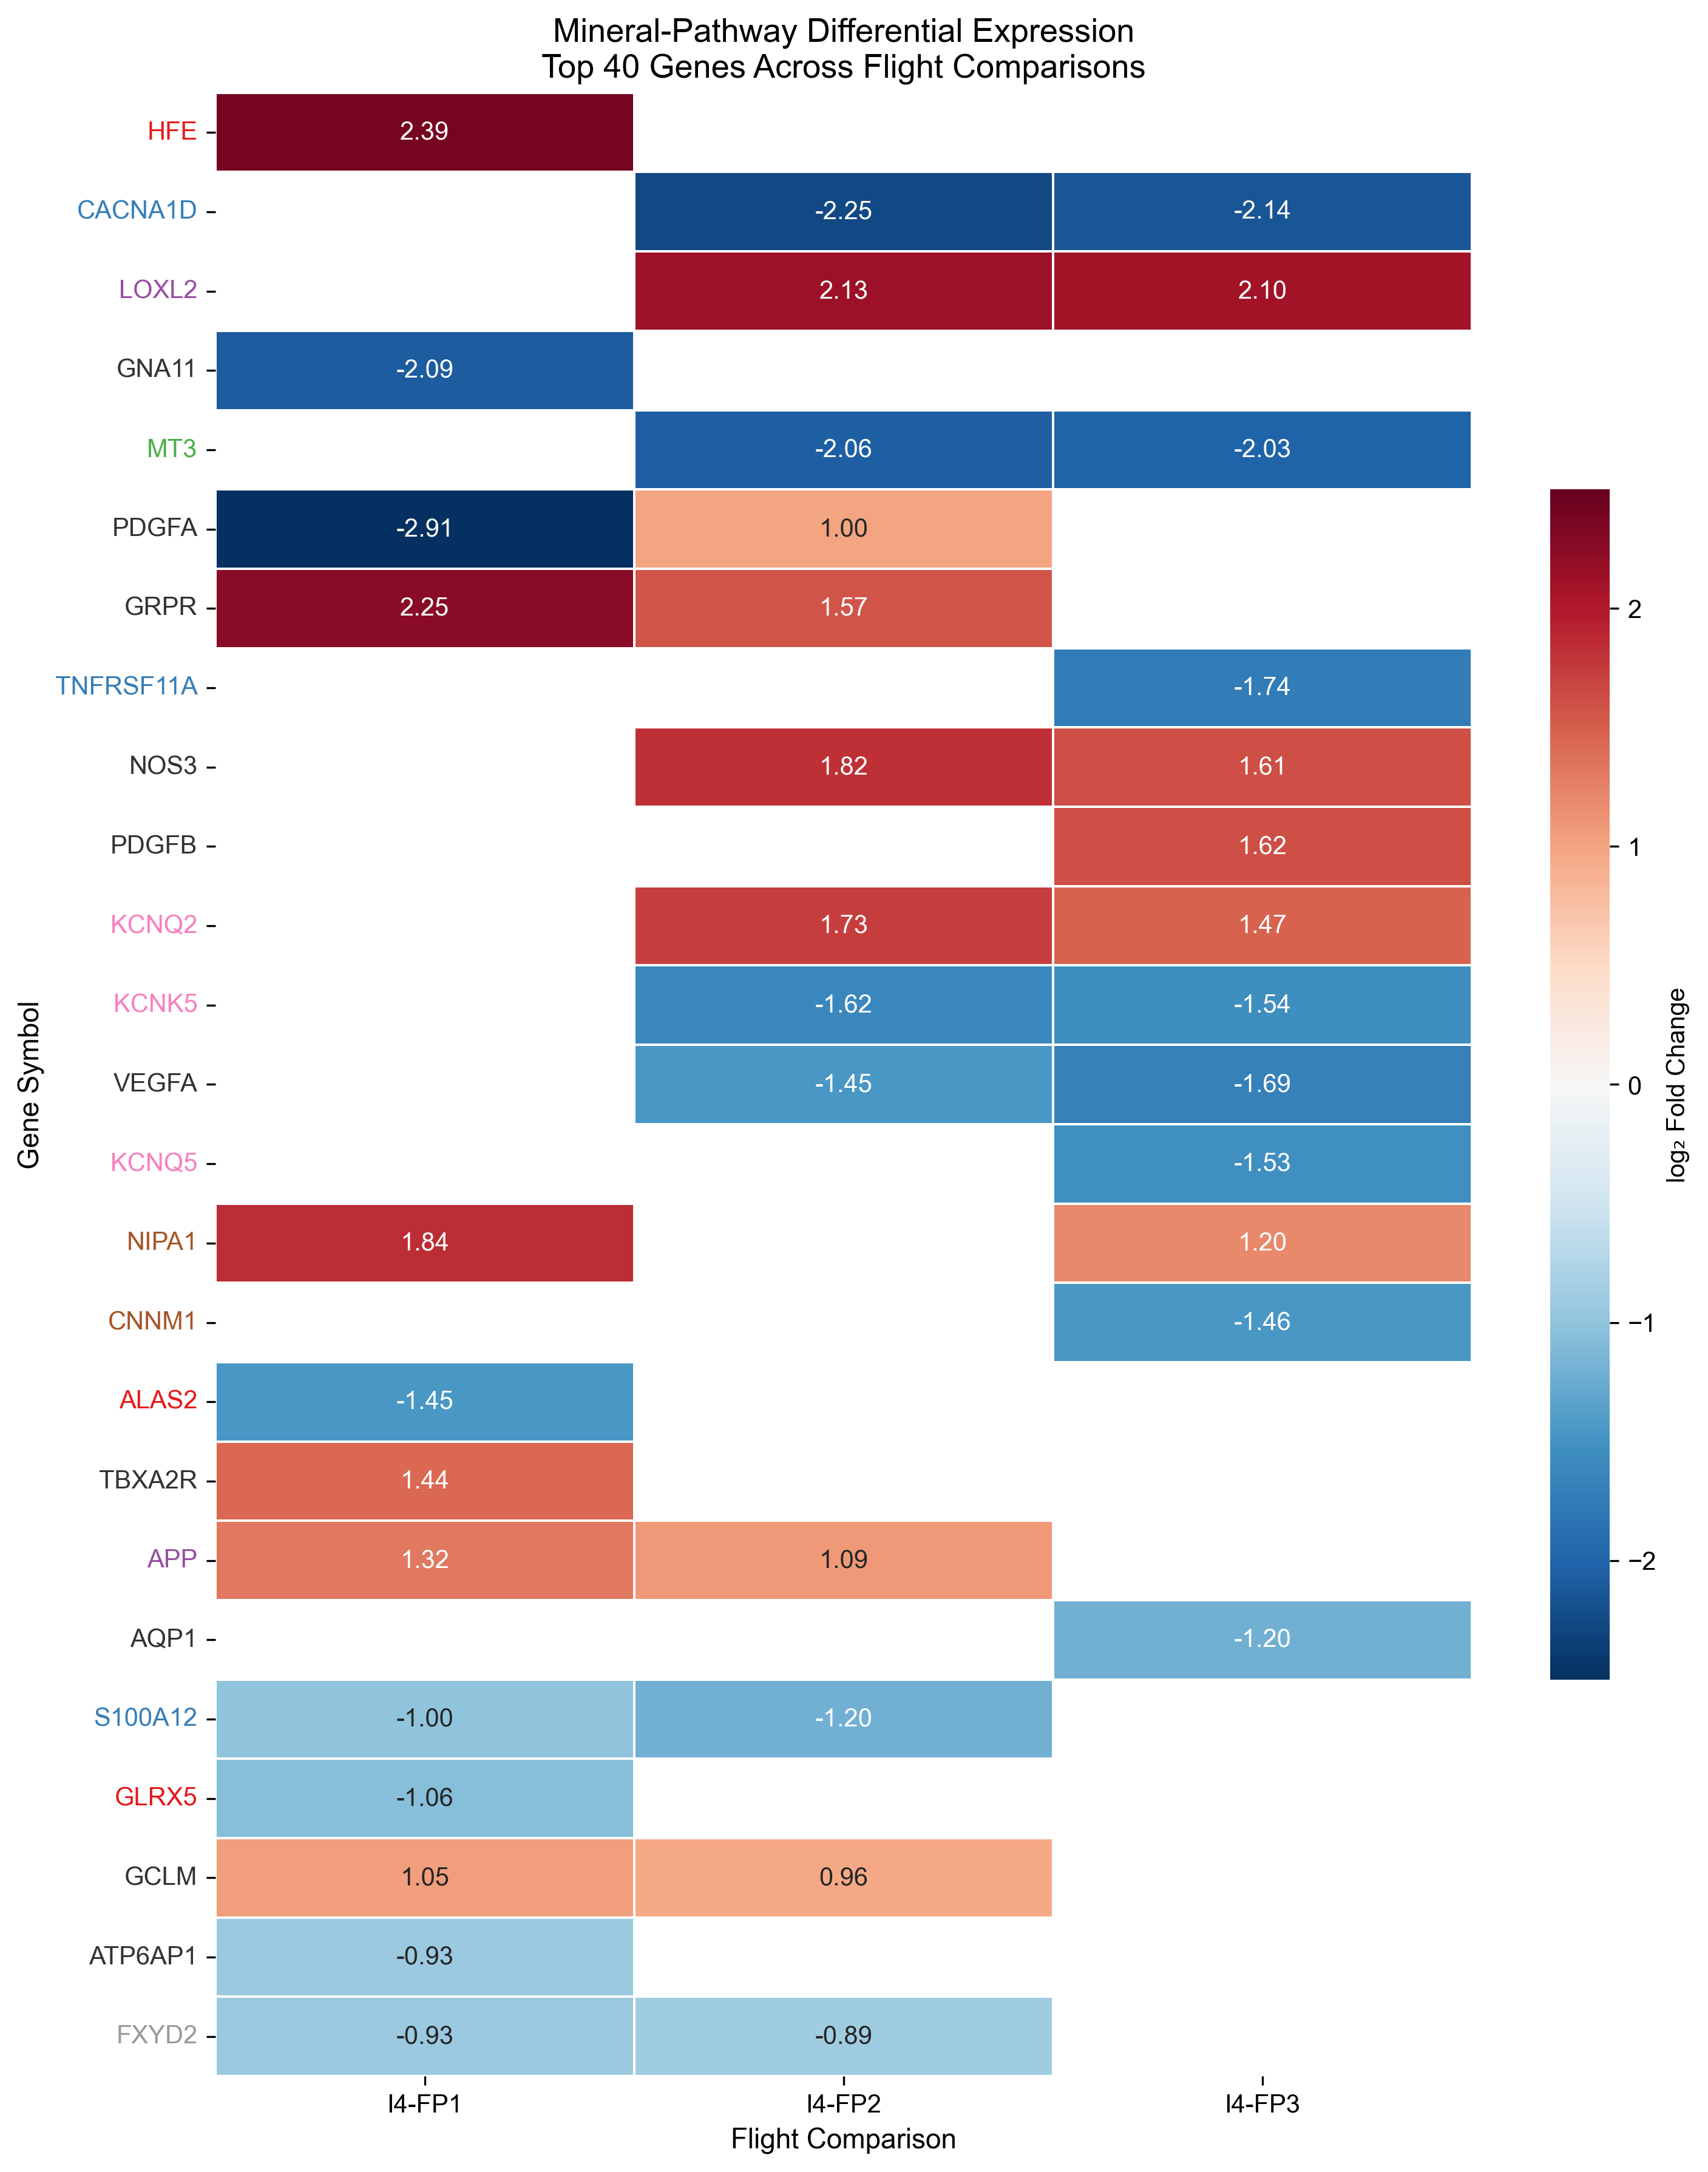
\includegraphics[width=\textwidth]{figures/fig1_heatmap_mineral_de.png}
\caption{}
\end{subfigure}
\hfill
\begin{subfigure}{0.43\textwidth}
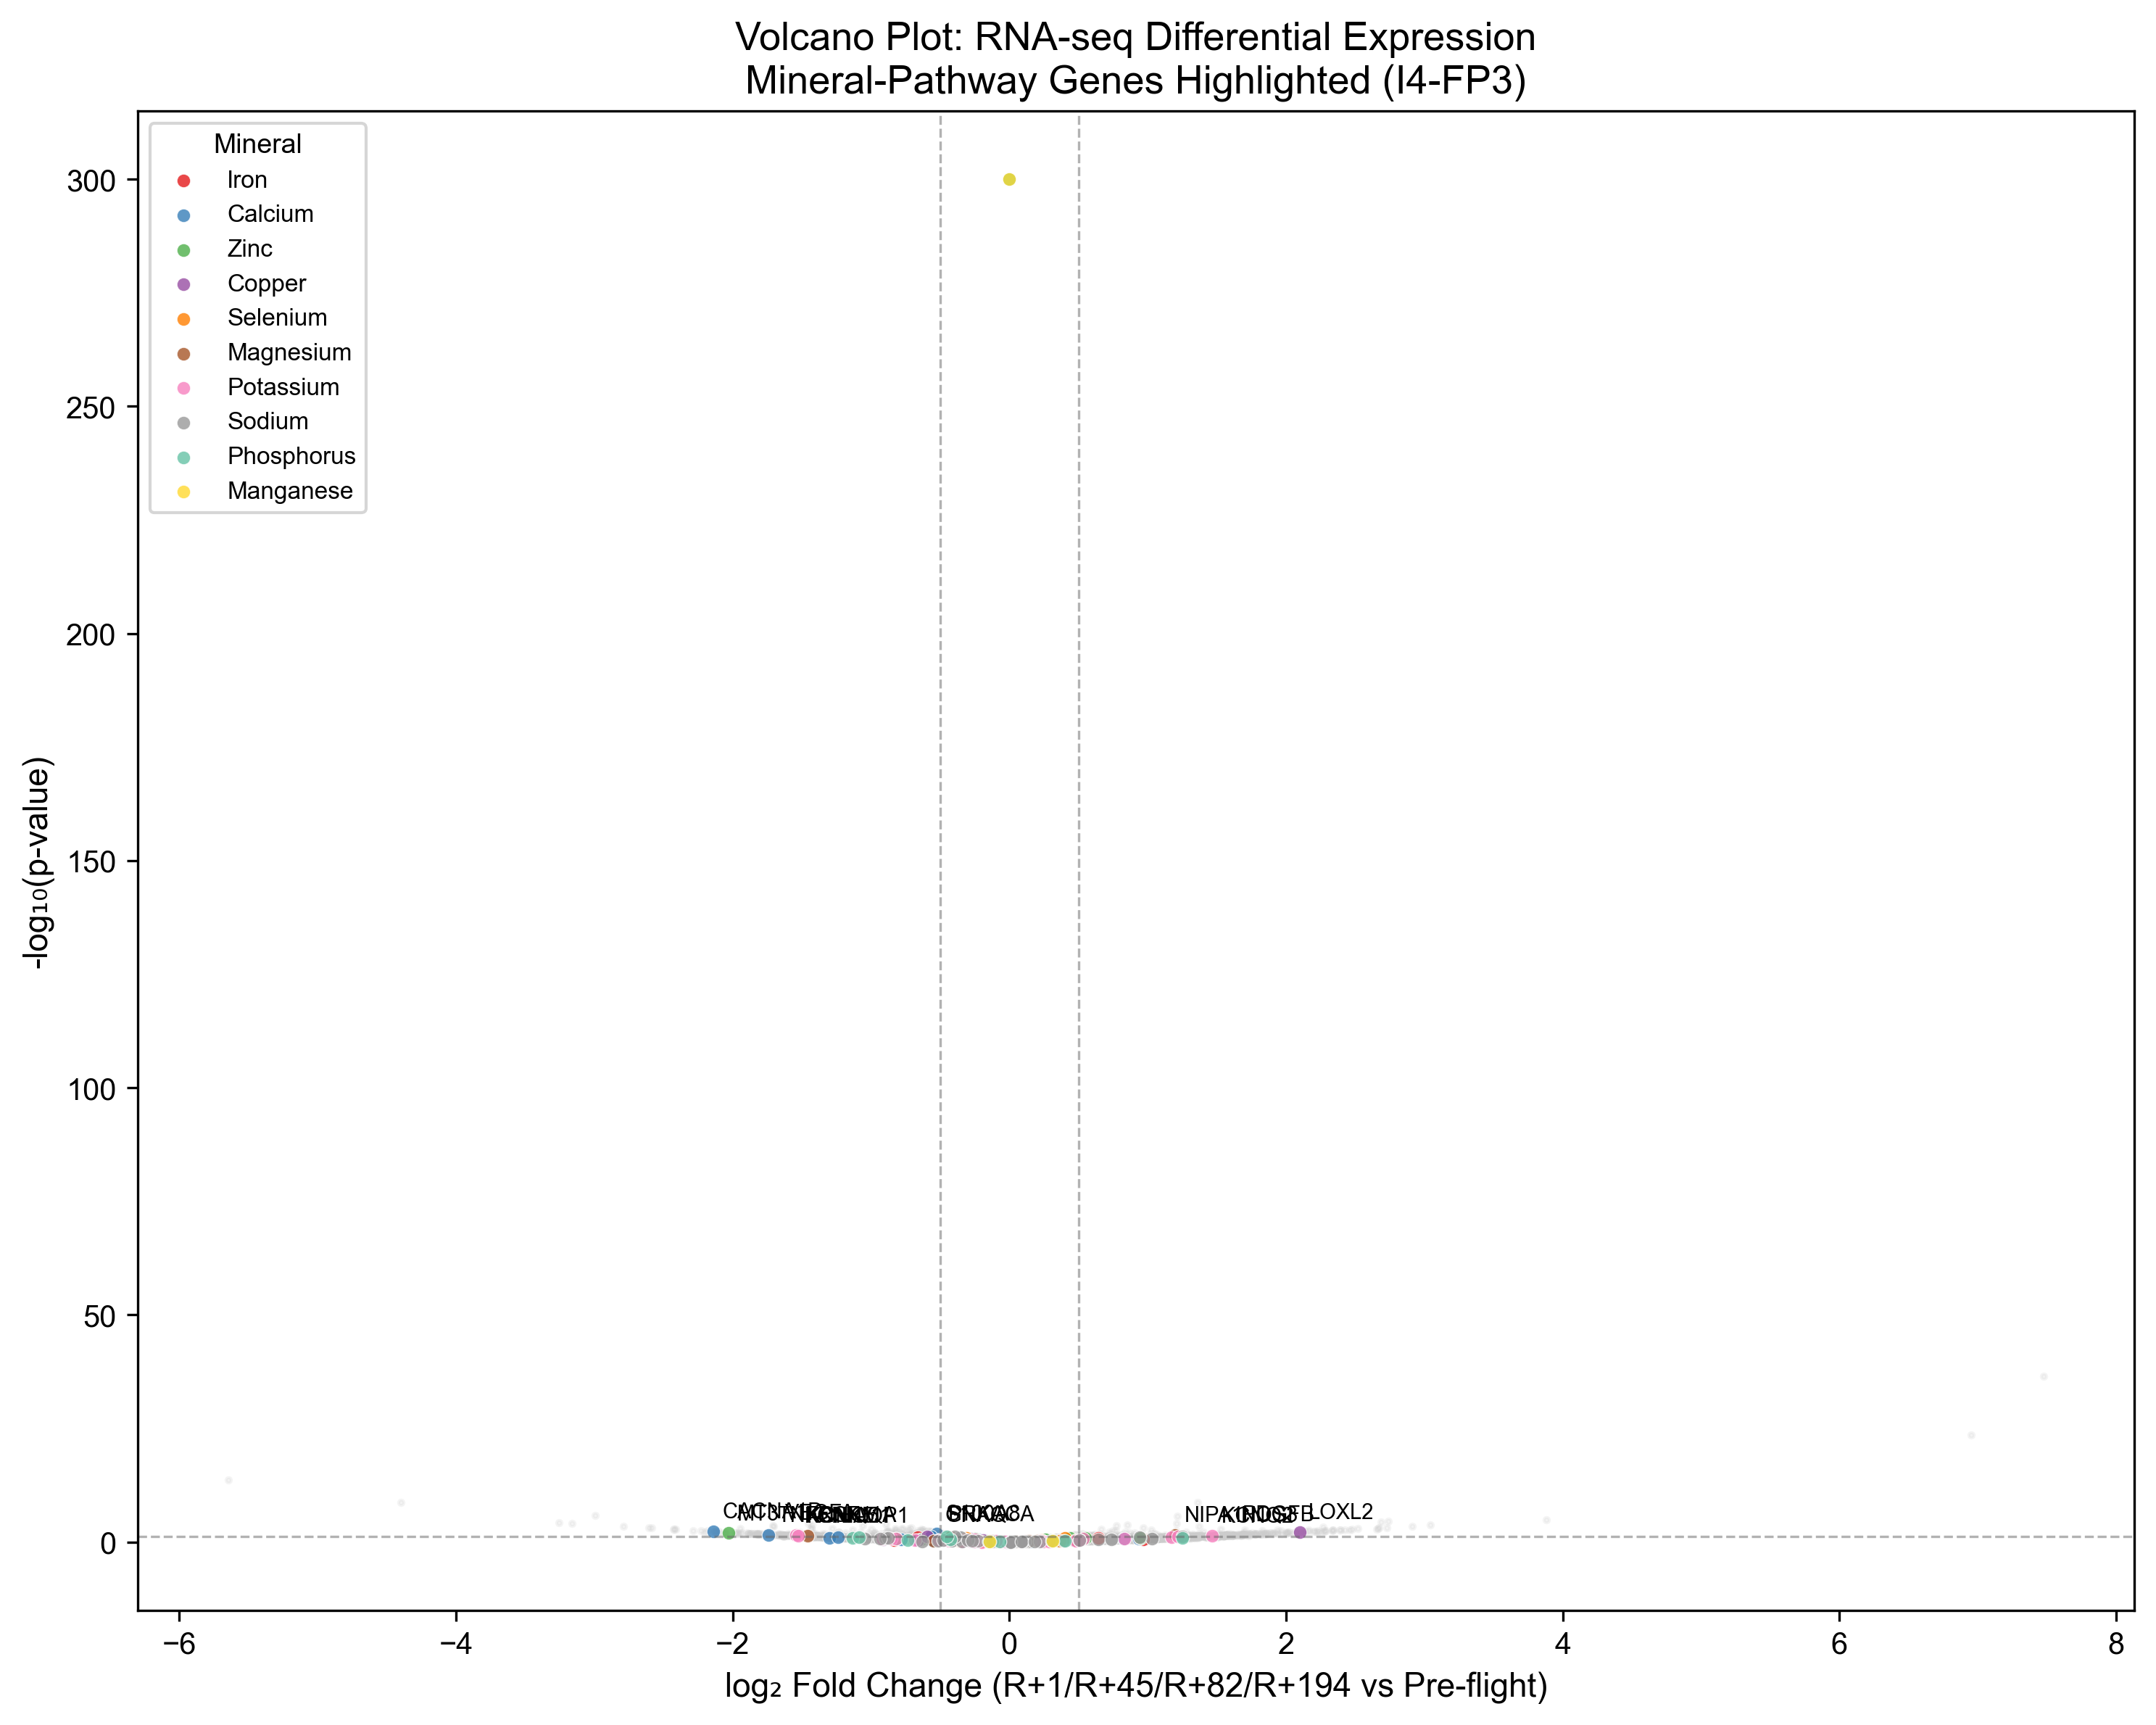
\includegraphics[width=\textwidth]{figures/fig2_volcano_rnaseq.png}
\caption{}
\end{subfigure}

\vspace{0.5em}
\begin{subfigure}{0.85\textwidth}
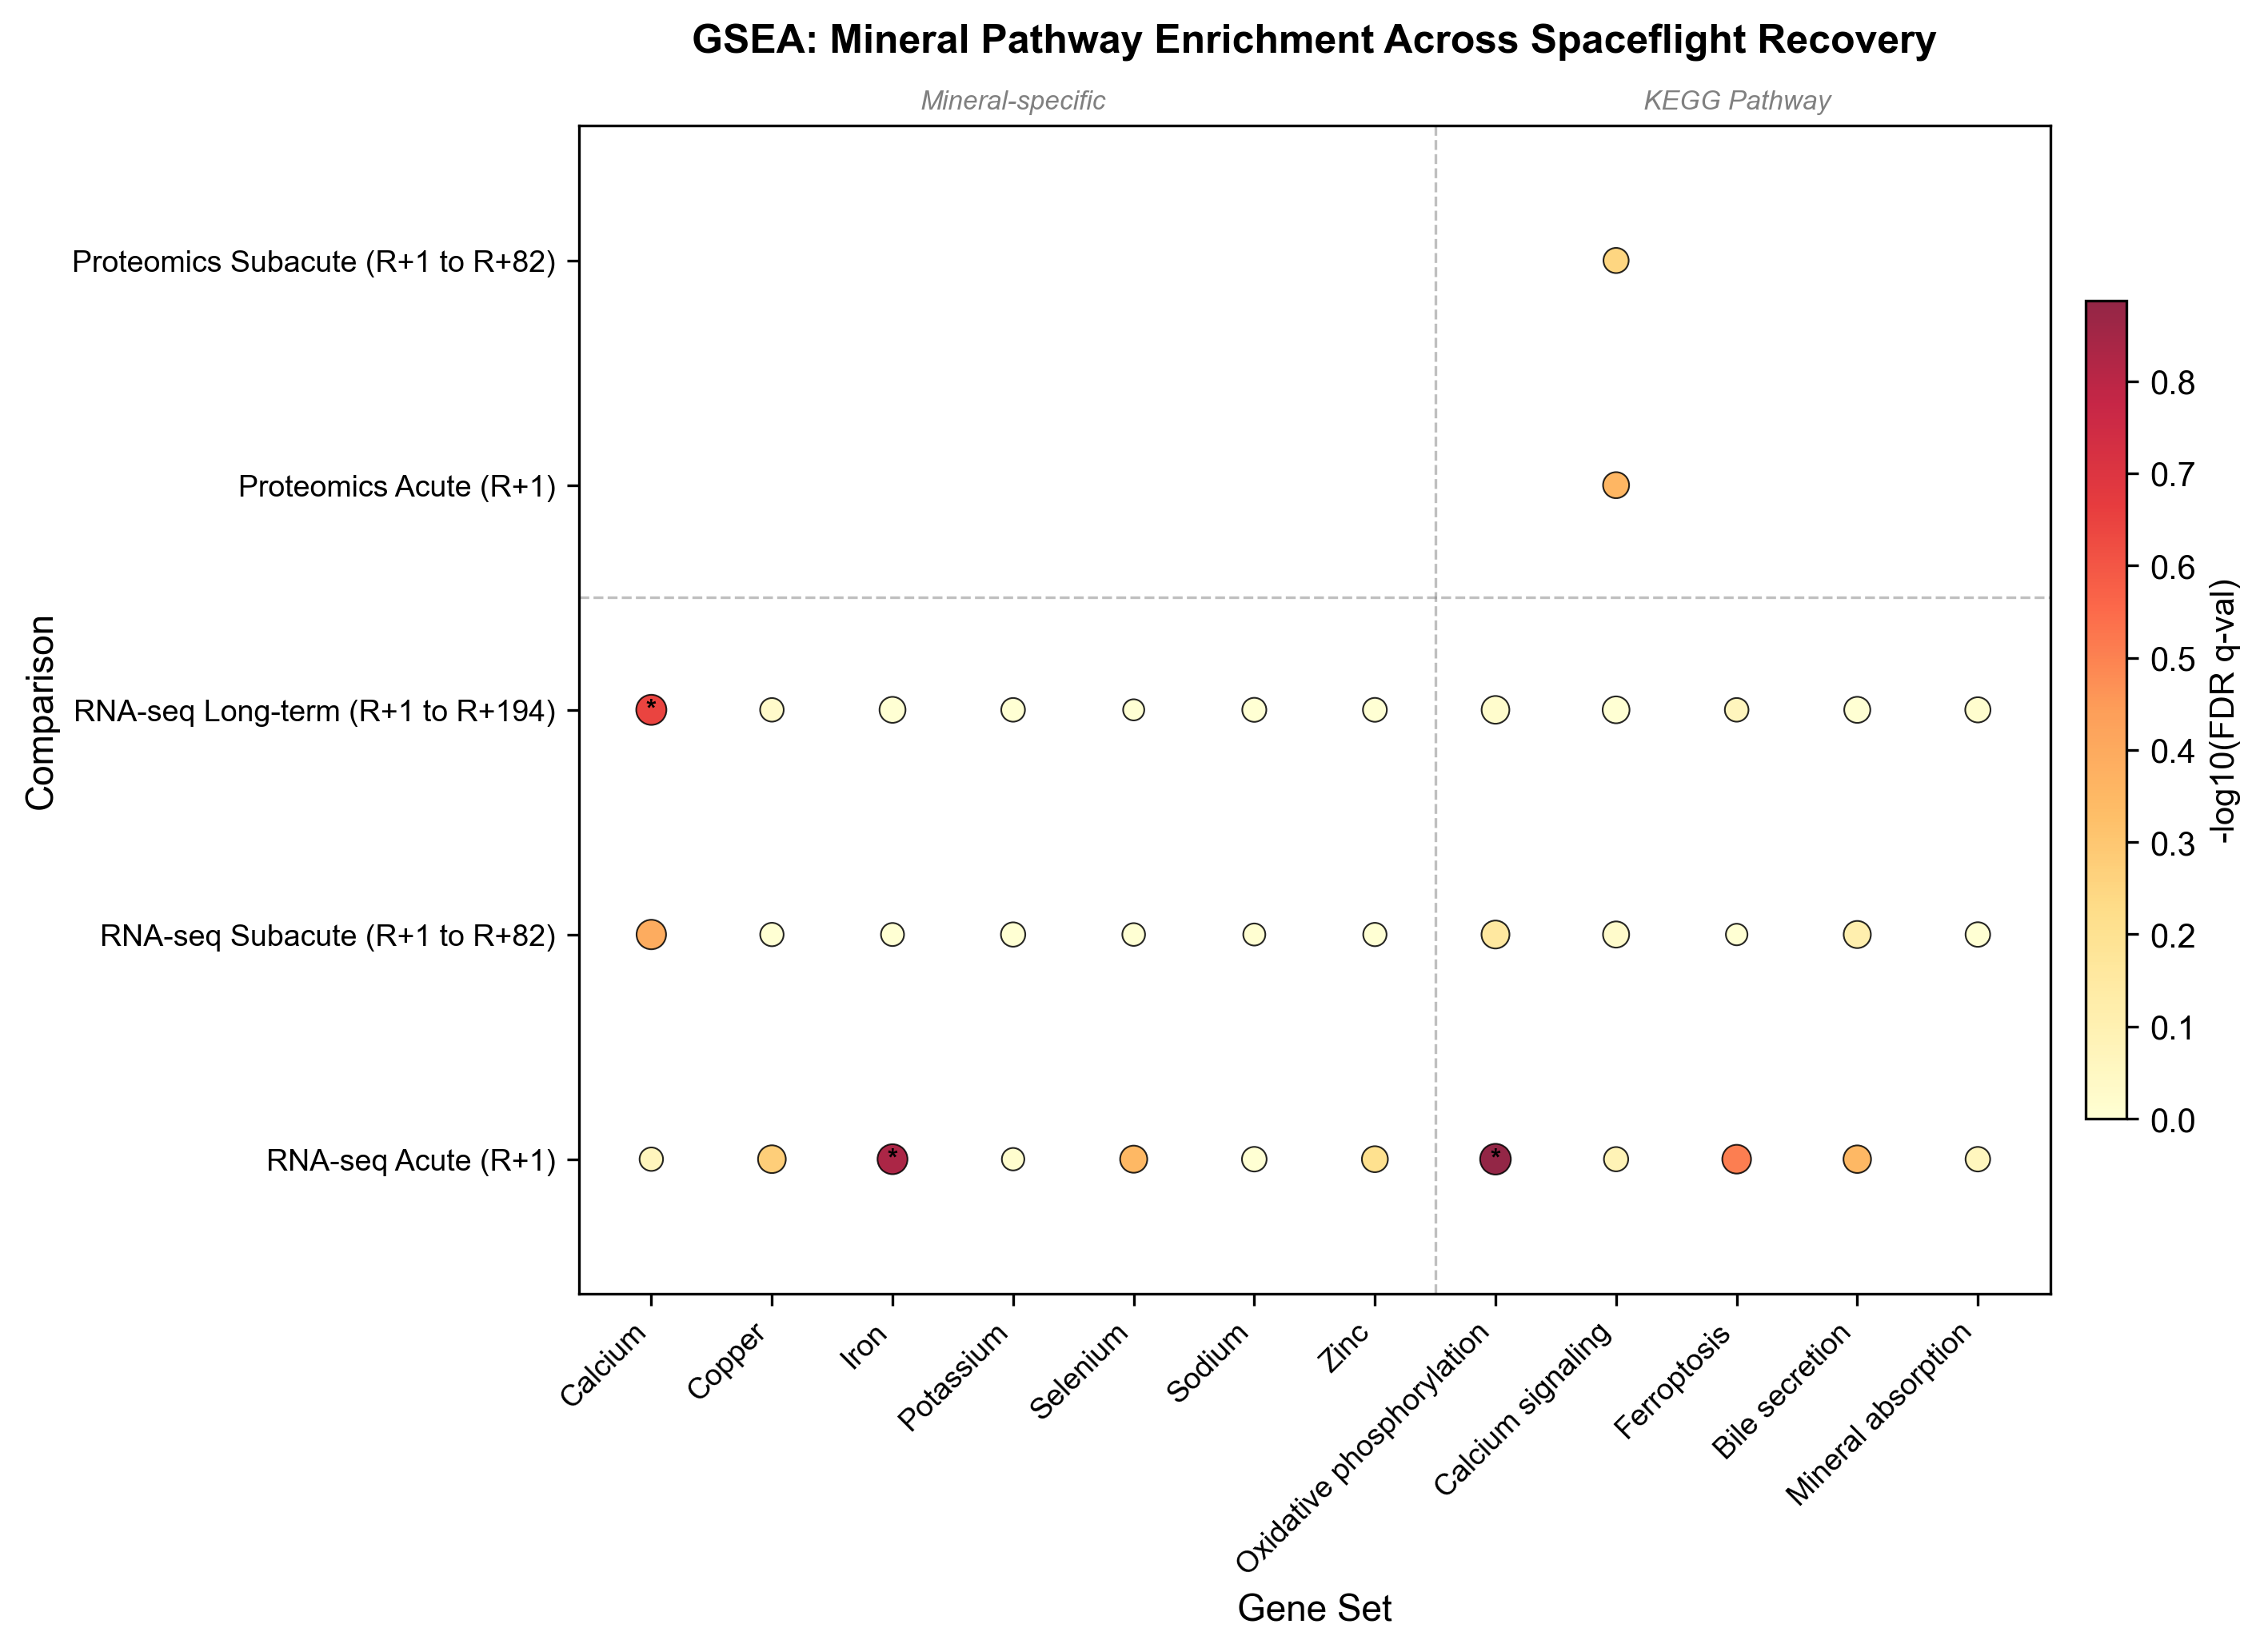
\includegraphics[width=\textwidth]{figures/figS1_gsea_enrichment.png}
\caption{}
\end{subfigure}
\caption{Mineral-pathway differential expression. (a) Heatmap of significant mineral-pathway DE genes ($|\log_2\text{FC}| > 0.5$, $p < 0.05$) across RNA-seq and proteomics comparisons. Gene annotations indicate primary mineral associations. (b) Volcano plot of RNA-seq differential expression (I4-FP1: R+1 vs.\ pre-flight), with mineral-pathway genes highlighted by mineral association. (c) GSEA enrichment of mineral-specific gene sets and KEGG pathways across flight comparisons, showing normalized enrichment scores and significance.}
\label{fig:de_heatmap}
\end{figure}

The most consistent findings were: \textbf{Copper pathway} --- APP (amyloid precursor protein, copper-binding) was up-regulated in proteomics ($\log_2\text{FC} = 1.32$, FDR $= 0.001$), while LOX and LOXL1 (copper-dependent lysyl oxidases) were down-regulated. LOXL2 was up-regulated in RNA-seq ($\log_2\text{FC} = 2.10$). Lysyl oxidases are critical for collagen cross-linking and connective tissue integrity\textsuperscript{7}. \textbf{Iron pathway} --- ALAS2 (erythroid-specific aminolevulinate synthase) was down-regulated ($\log_2\text{FC} = -1.45$, FDR $= 0.008$), while HFE (hemochromatosis gene) was up-regulated ($\log_2\text{FC} = 2.39$). GLRX5 was also down-regulated. These changes are consistent with the space-flight anemia and increased iron availability reported in astronauts\textsuperscript{6}. \textbf{Magnesium pathway} --- NIPA1 was up-regulated ($\log_2\text{FC} = 1.84$). \textbf{Calcium pathway} --- S100A8, S100A9, and S100A12 (calcium-binding calgranulins) were down-regulated in proteomics and RNA-seq; S100A8/A9 form calprotectin, a key innate immune mediator\textsuperscript{8}. CACNA1D (voltage-gated calcium channel) showed the largest fold change ($\log_2\text{FC} = -2.25$ in I4-FP2, $-2.14$ in I4-FP3), potentially reflecting cellular adaptation to mechanical unloading, which alters mechanotransduction signalling\textsuperscript{9}. \textbf{Zinc pathway} --- MT2A and MT3 (metallothioneins) were down-regulated ($\log_2\text{FC} = -0.75$ to $-2.03$). \textbf{Potassium pathway} --- KCNQ2 was up-regulated ($\log_2\text{FC} = 1.73$), while FXYD2 (sodium/potassium transport regulator) was down-regulated in proteomics.

Gene set enrichment analysis (GSEA) revealed down-regulation of oxidative phosphorylation (NES $= -1.63$, NOM $p = 0.002$) and the iron mineral gene set (NES $= -1.53$, NOM $p = 0.037$) in the I4-FP1 comparison, while ferroptosis showed a trend toward up-regulation (NES $= 1.37$, NOM $p = 0.052$). The calcium gene set trended toward down-regulation in the later comparisons (I4-FP2: NES $= -1.46$, NOM $p = 0.033$; I4-FP3: NES $= -1.55$, NOM $p = 0.017$, FDR $q = 0.23$; Figure~\ref{fig:de_heatmap}c). Time-resolved pathway activation patterns are shown in Supplementary Figure~S2.

\subsubsection{NHANES iron status reference and CBC correlations}

Because the astronaut clinical panel did not include serum iron, ferritin, transferrin saturation, or total iron-binding capacity (TIBC), we extended the NHANES reference to include these four iron status markers, providing population context for the iron-pathway transcriptomic findings. Serum iron (LBXSIR) was available from the Standard Biochemistry Profile across all three cycles ($n = 5{,}435$); ferritin (LBXFER) was available from 2015--2018 ($n = 2{,}190$); and transferrin saturation (LBDPCT) and TIBC (LBDTIB) were available from 2017--2018 only ($n = 1{,}678$), as the NHANES 2013--2014 cycle did not include ferritin or TIBC files. Reference intervals (P2.5--P97.5) were: serum iron 24.0--160.0~$\mu$g/dL (mean 83.3, SD 36.0); ferritin 6.4--565.6~ng/mL (mean 147.1, SD 200.9); transferrin saturation 7.0--55.0\% (mean 27.4, SD 11.7); and TIBC 237.9--442.2~$\mu$g/dL (mean 324.6, SD 50.9).

To quantify the relationship between iron status and the hematological markers available in both NHANES and astronaut data, we computed Pearson correlations between each iron marker and six CBC parameters (hemoglobin, hematocrit, RBC count, MCH, MCHC, MCV) within the NHANES reference population (age 40--60, all sexes; Figure~\ref{fig:iron_ref}). Hemoglobin was the strongest CBC correlate of iron status: serum iron vs.\ hemoglobin $r = 0.424$ ($p = 4.6 \times 10^{-236}$, $n = 5{,}424$), transferrin saturation vs.\ hemoglobin $r = 0.412$ ($p = 1.4 \times 10^{-69}$, $n = 1{,}677$), and ferritin vs.\ hemoglobin $r = 0.274$ ($p = 5.0 \times 10^{-39}$, $n = 2{,}187$). TIBC showed a negative correlation with hemoglobin ($r = -0.223$, $p = 2.9 \times 10^{-20}$), consistent with the inverse relationship between iron-binding capacity and iron stores in iron deficiency. MCH showed similarly strong correlations (serum iron $r = 0.379$; transferrin saturation $r = 0.408$). Of 24 correlations tested, 23 reached $p < 0.05$ (only TIBC vs.\ RBC count was non-significant, $r = -0.005$, $p = 0.85$). These population-level correlations establish hemoglobin as a robust proxy for iron status, strengthening the link between the modest astronaut hemoglobin deviations and the iron-pathway transcriptional changes (ALAS2 down-regulation, HFE up-regulation) observed in the transcriptomic data.

\begin{figure}[H]
\centering
\begin{subfigure}{0.62\textwidth}
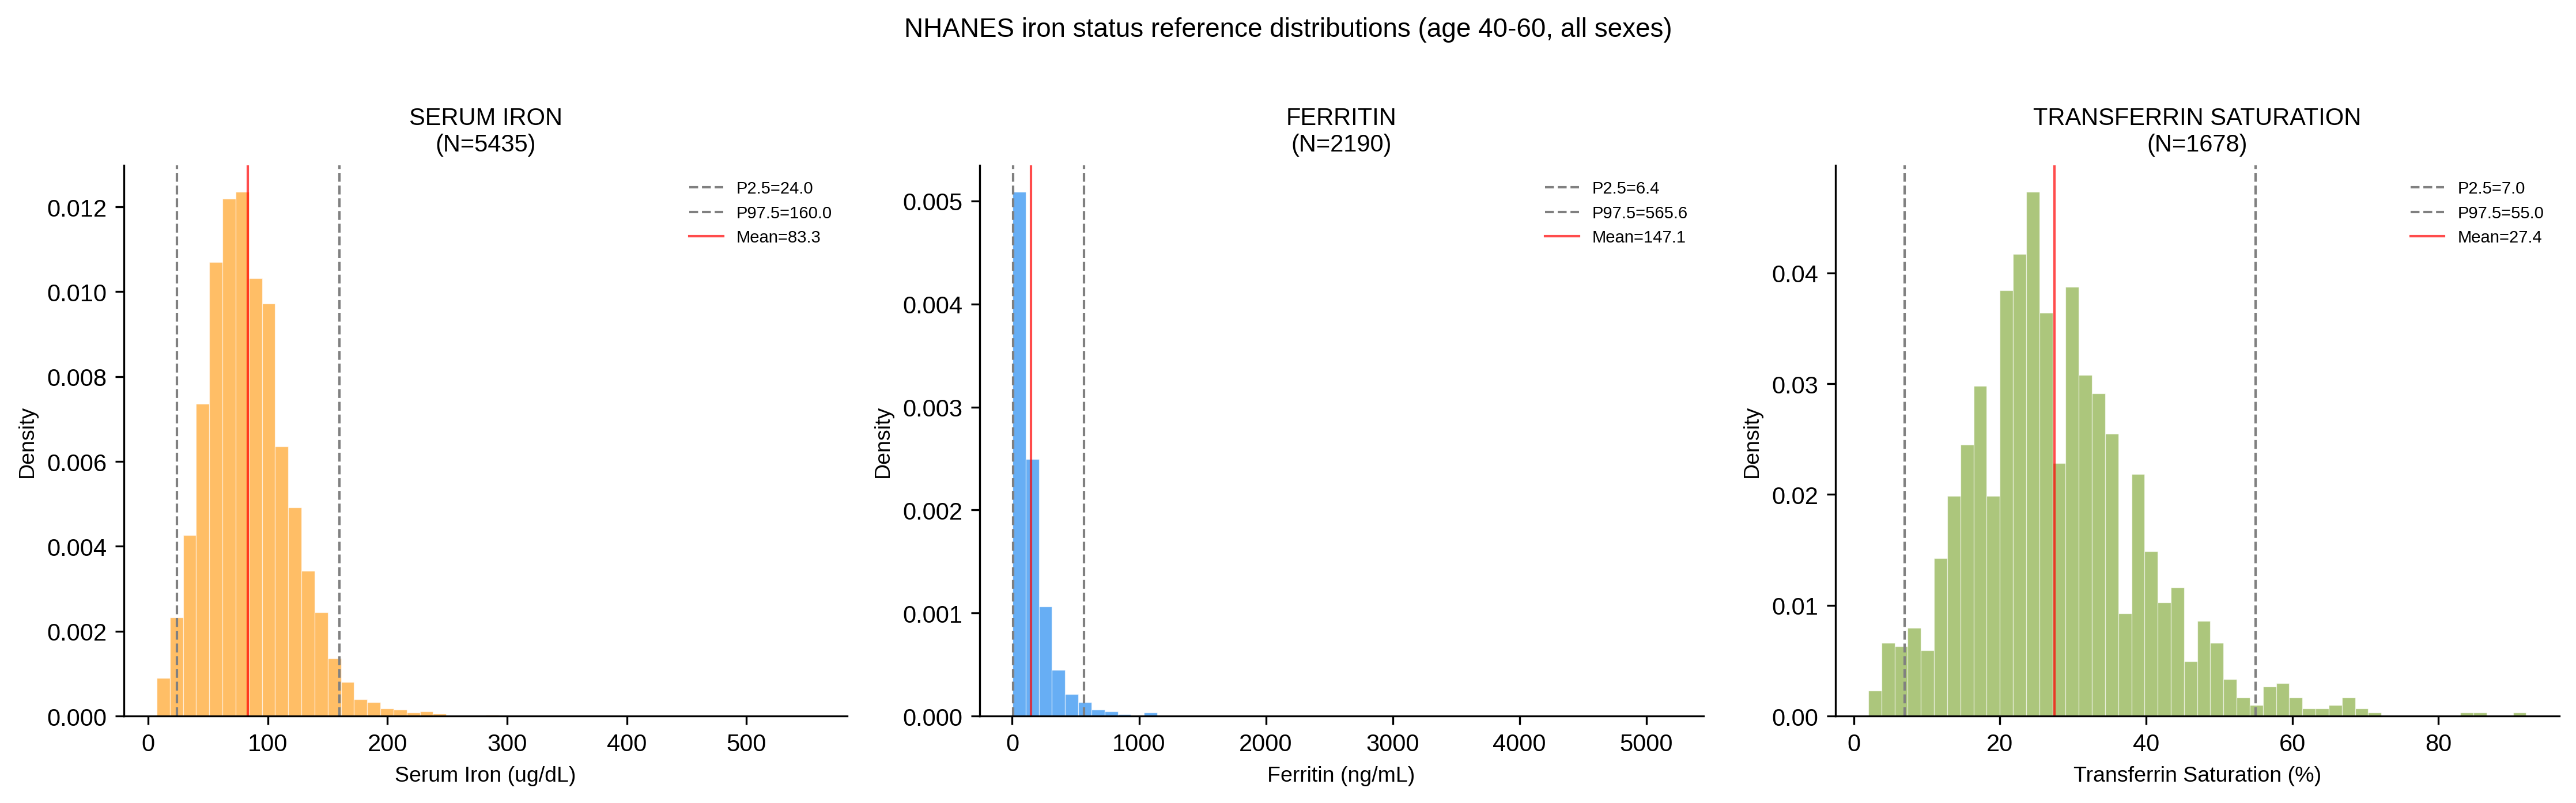
\includegraphics[width=\textwidth]{figures/dl_iron_reference_panel.png}
\caption{}
\end{subfigure}
\hfill
\begin{subfigure}{0.36\textwidth}
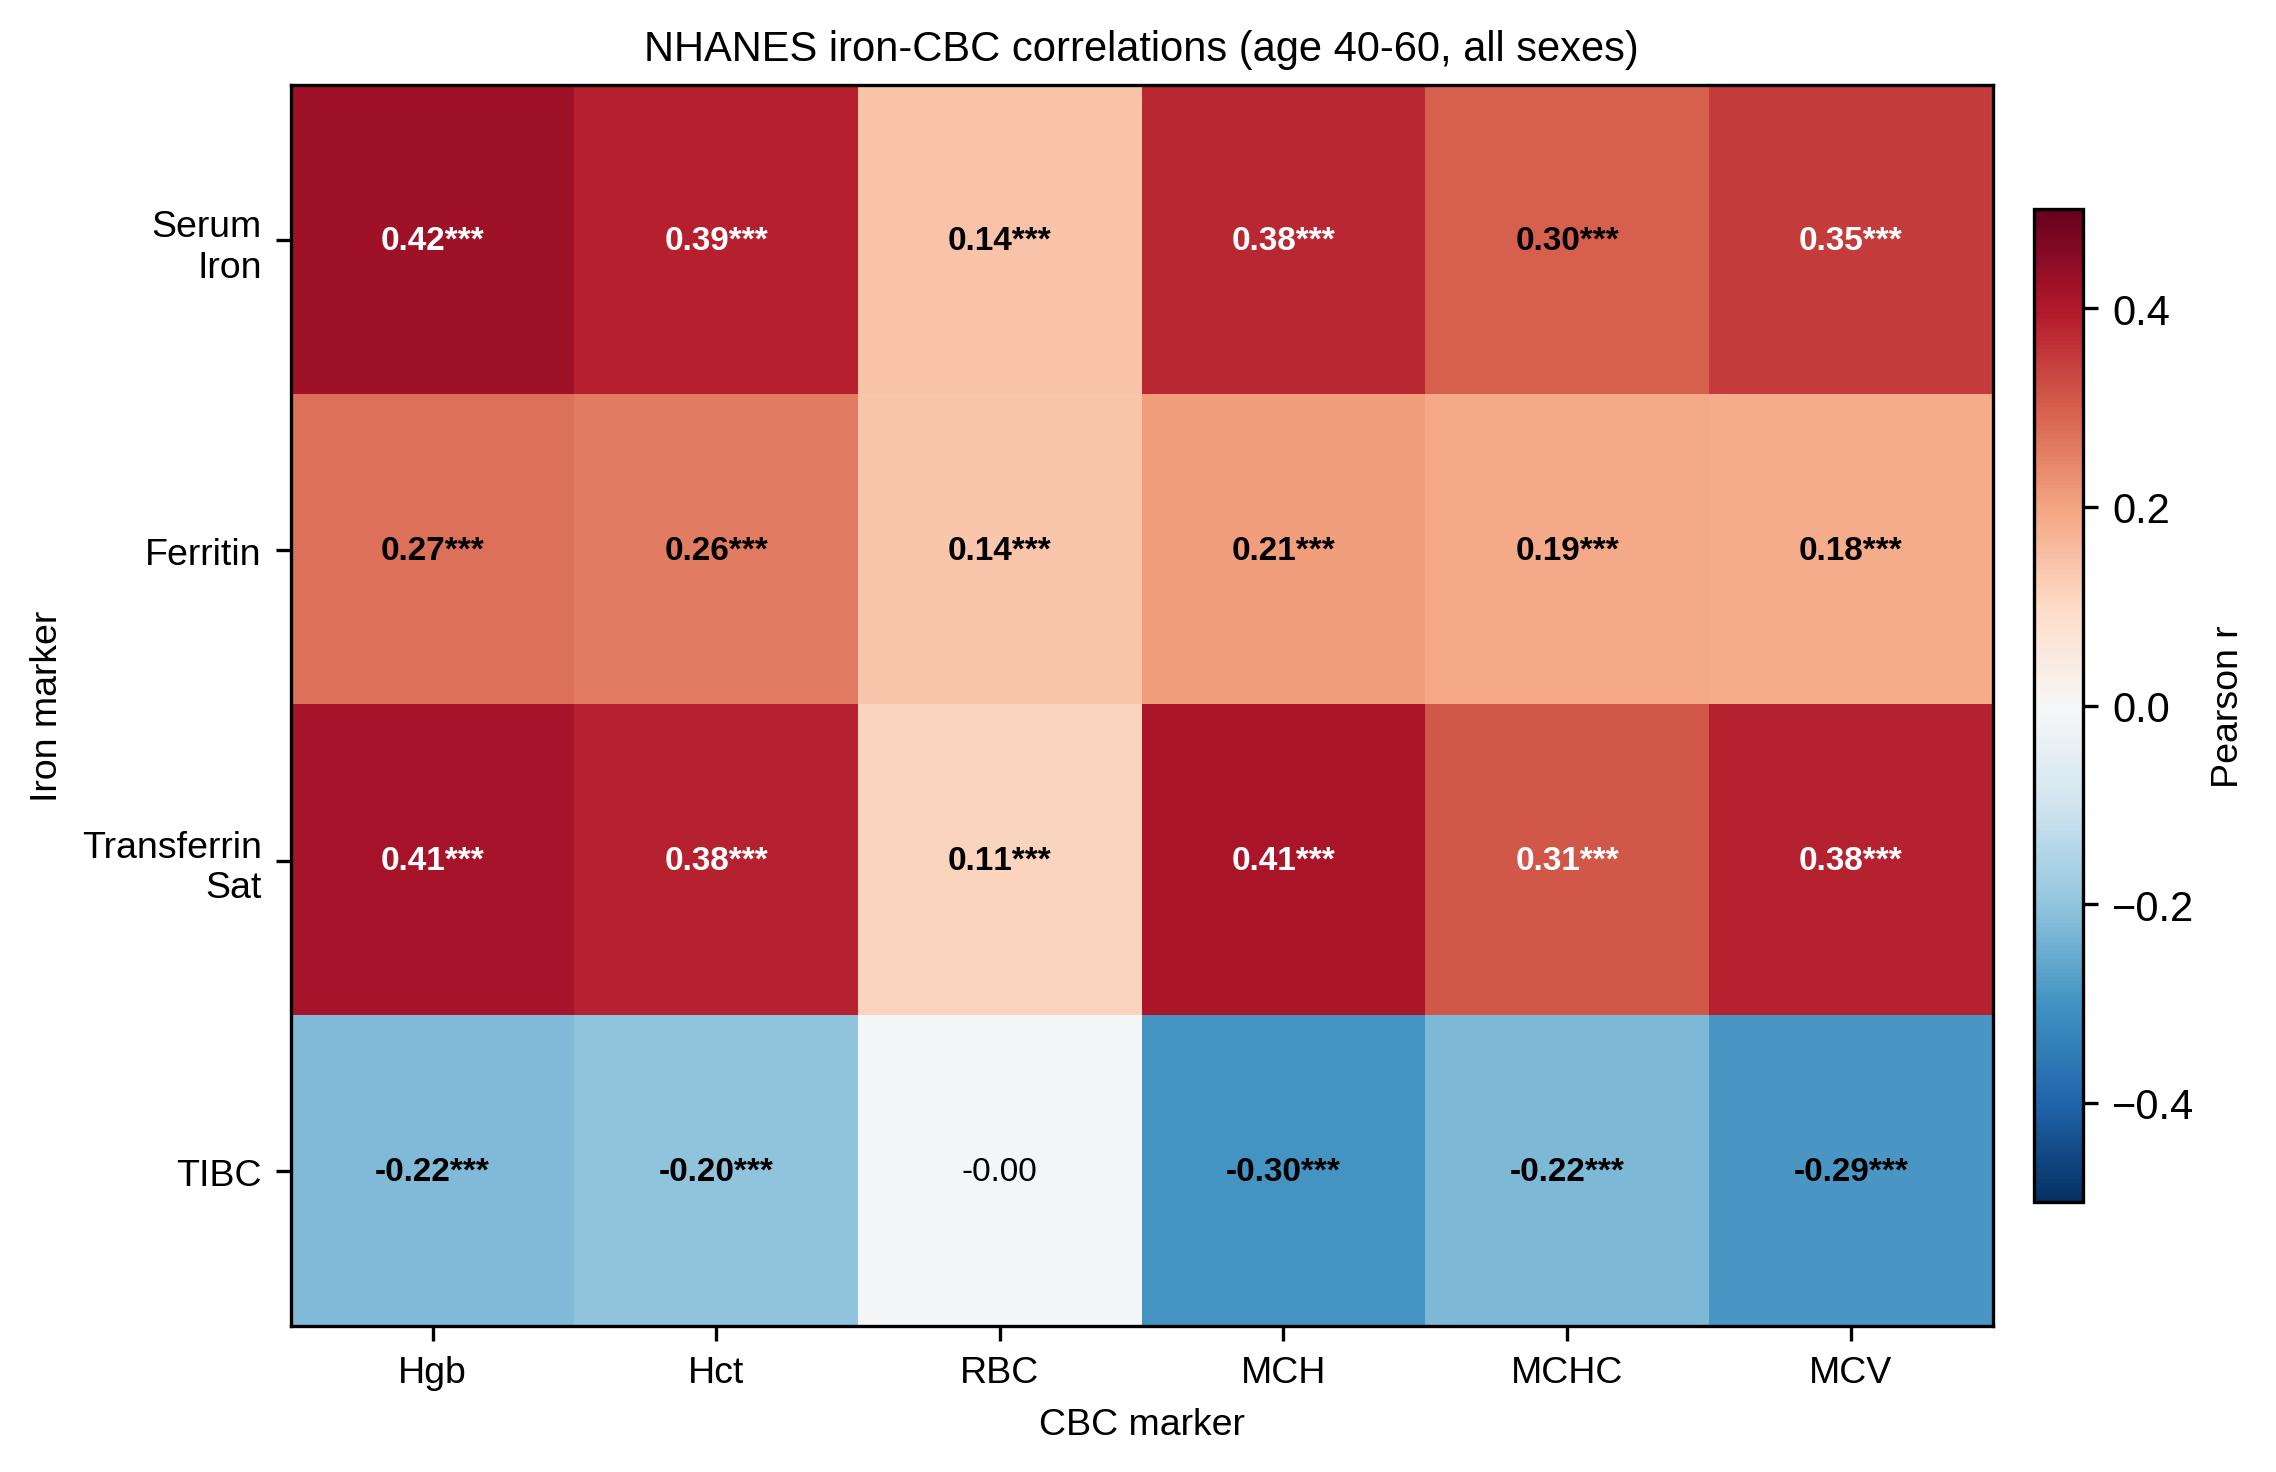
\includegraphics[width=\textwidth]{figures/dl_iron_cbc_correlation_heatmap.png}
\caption{}
\end{subfigure}
\caption{NHANES iron status reference and CBC correlations. (a) Reference distributions of serum iron, ferritin, and transferrin saturation in the NHANES population (age 40--60, all sexes), with P2.5, P97.5, and mean indicated by dashed lines. (b) Pearson correlation heatmap between four iron status markers (rows) and six CBC parameters (columns). Asterisks denote significance: ***$p < 0.001$, **$p < 0.01$, *$p < 0.05$. Hemoglobin and MCH show the strongest correlations with iron status markers, while TIBC is negatively correlated with all CBC parameters except RBC count.}
\label{fig:iron_ref}
\end{figure}

\subsection{Machine learning: mineral-pathway genes predict serum mineral levels}

We evaluated whether mineral-pathway gene expression carries predictive information about serum mineral levels using two complementary machine learning approaches.

\subsubsection{Regression analysis (mineral level prediction)}

Four regressors (Ridge, SVR-Linear, SVR-RBF, RandomForest) were trained to predict serum calcium, potassium, sodium, and hemoglobin (iron proxy) from mineral-pathway gene expression under leave-one-out cross-validation (LOO-CV, $n = 16$). The top 200 genes by variance were used as features. Potassium was predicted with $r = 0.50$ ($R^2 = 0.12$, Ridge regression) and sodium with $r = 0.46$ ($R^2 = 0.19$, SVR-Linear). Hemoglobin was predicted with $r = 0.48$ (SVR-Linear), though the negative $R^2$ ($-0.62$) indicates the model performs worse than the mean baseline on held-out samples. Calcium showed no predictive signal ($r = -0.02$).

Permutation importance analysis identified \textit{CAMK4} (calcium signaling), \textit{SLC30A7} (zinc transporter), \textit{SELENOW} (selenium protein), \textit{SLC11A1} (iron transporter), and \textit{ALPL} (calcium/phosphorus) as top predictive genes for potassium, and \textit{CAMK4}, \textit{ITPKB}, \textit{SLC2A1}, and \textit{PPP3R1} for sodium (Figure~\ref{fig:ml_results}a). The contribution of genes from multiple mineral pathways to predicting individual minerals highlights the interconnectedness of mineral homeostasis systems.

\subsubsection{Classification analysis (flight vs.\ ground)}

A revised classification analysis addressed three issues in the initial pipeline: data leakage from feature selection outside cross-validation, lack of imbalance handling, and in-sample permutation importance. Class-weighted elastic-net logistic regression with nested LOO-CV was applied to all 784 mineral-pathway genes, with a 500-permutation significance test.

SVM with RBF kernel achieved AUC $= 1.0$ (perfect ranking) with permutation $p < 0.002$. However, the null distribution was non-standard (mean $= 0.121$), because \texttt{class\_weight='balanced'} biases the classifier toward specificity when labels are shuffled, inflating the apparent significance. The elastic-net models showed no discriminative signal (balanced AUC $= 0.06$--$0.35$, all $p > 0.67$), indicating that linear mineral-pathway gene expression cannot reliably separate flight from ground samples with $n = 4$.

Stability selection identified 16 genes selected in $\geq 50\%$ of LOO folds (Figure~\ref{fig:ml_results}b), enriched in iron metabolism (\textit{HFE} 88\%, \textit{SLC11A2} 81\%, \textit{ALAS2} 69\%, \textit{PCBP2} 69\%) and potassium transport (\textit{KCNE1} 94\%). These results are discovery-only and underpowered; the permutation null distribution and confusion matrices are provided in Supplementary Figure~S4.

\begin{figure}[H]
\centering
\begin{subfigure}{0.48\textwidth}
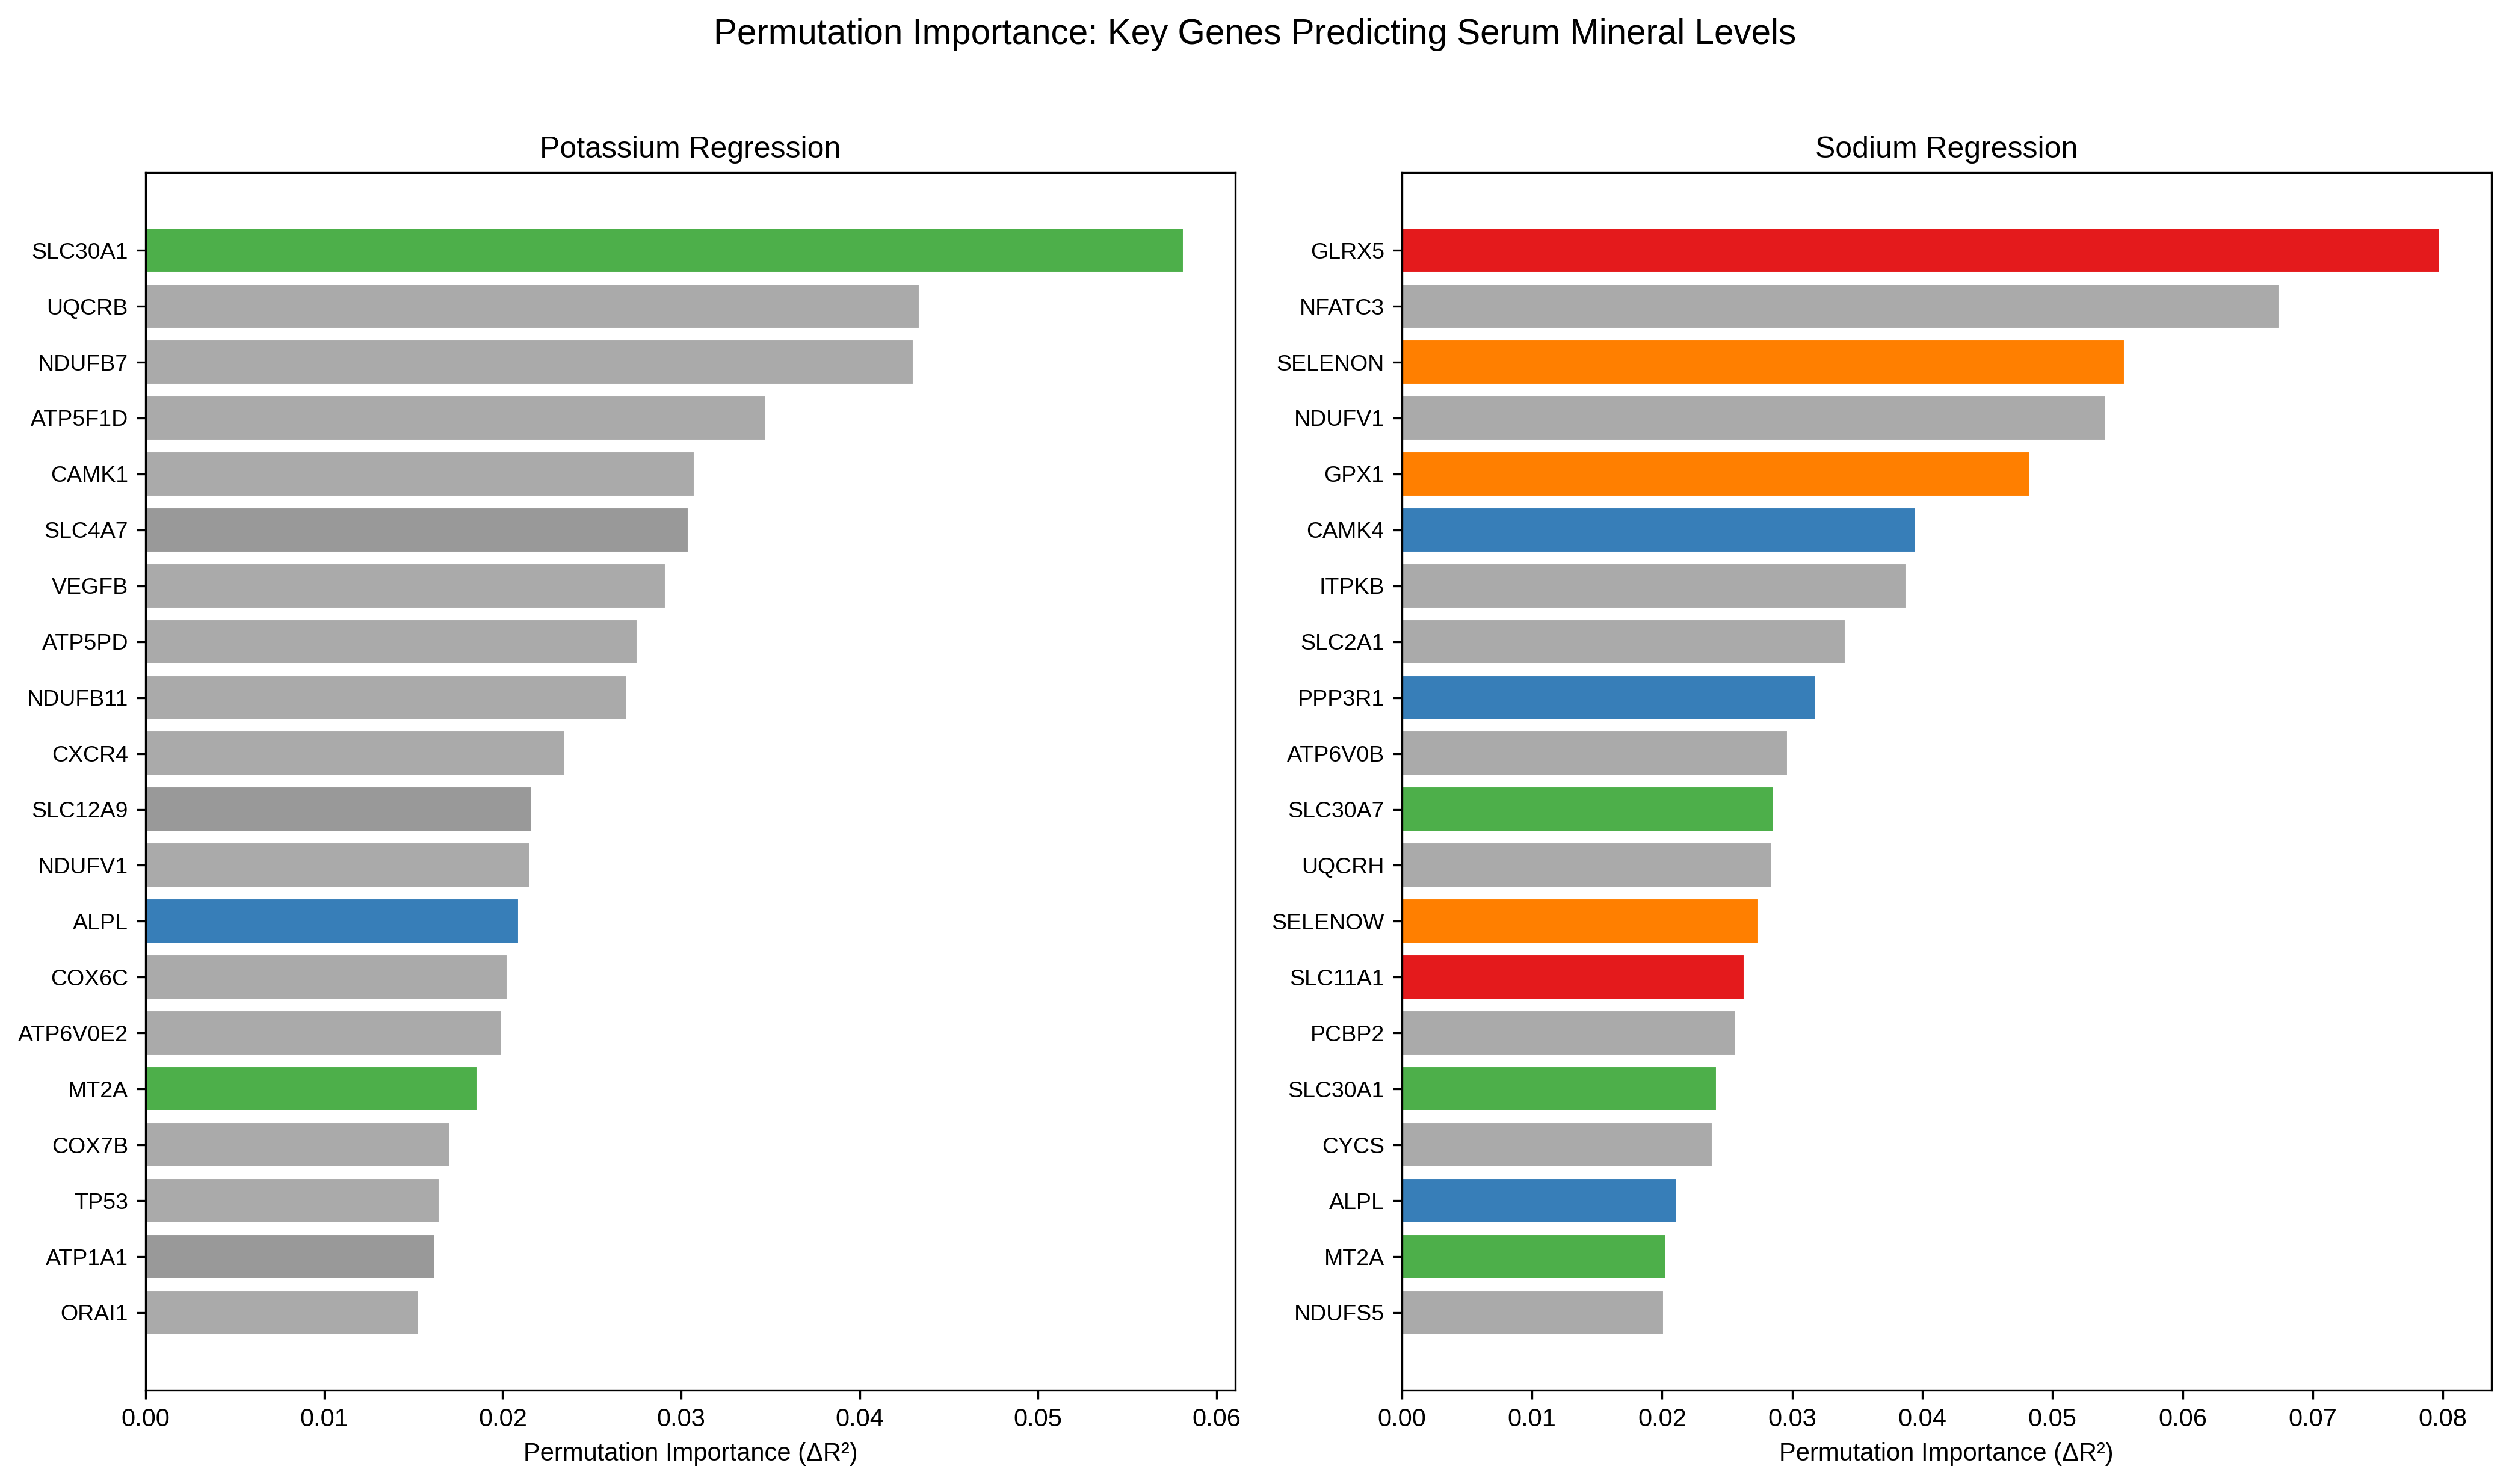
\includegraphics[width=\textwidth]{figures/fig3_barplot_importance.png}
\caption{}
\end{subfigure}
\hfill
\begin{subfigure}{0.48\textwidth}
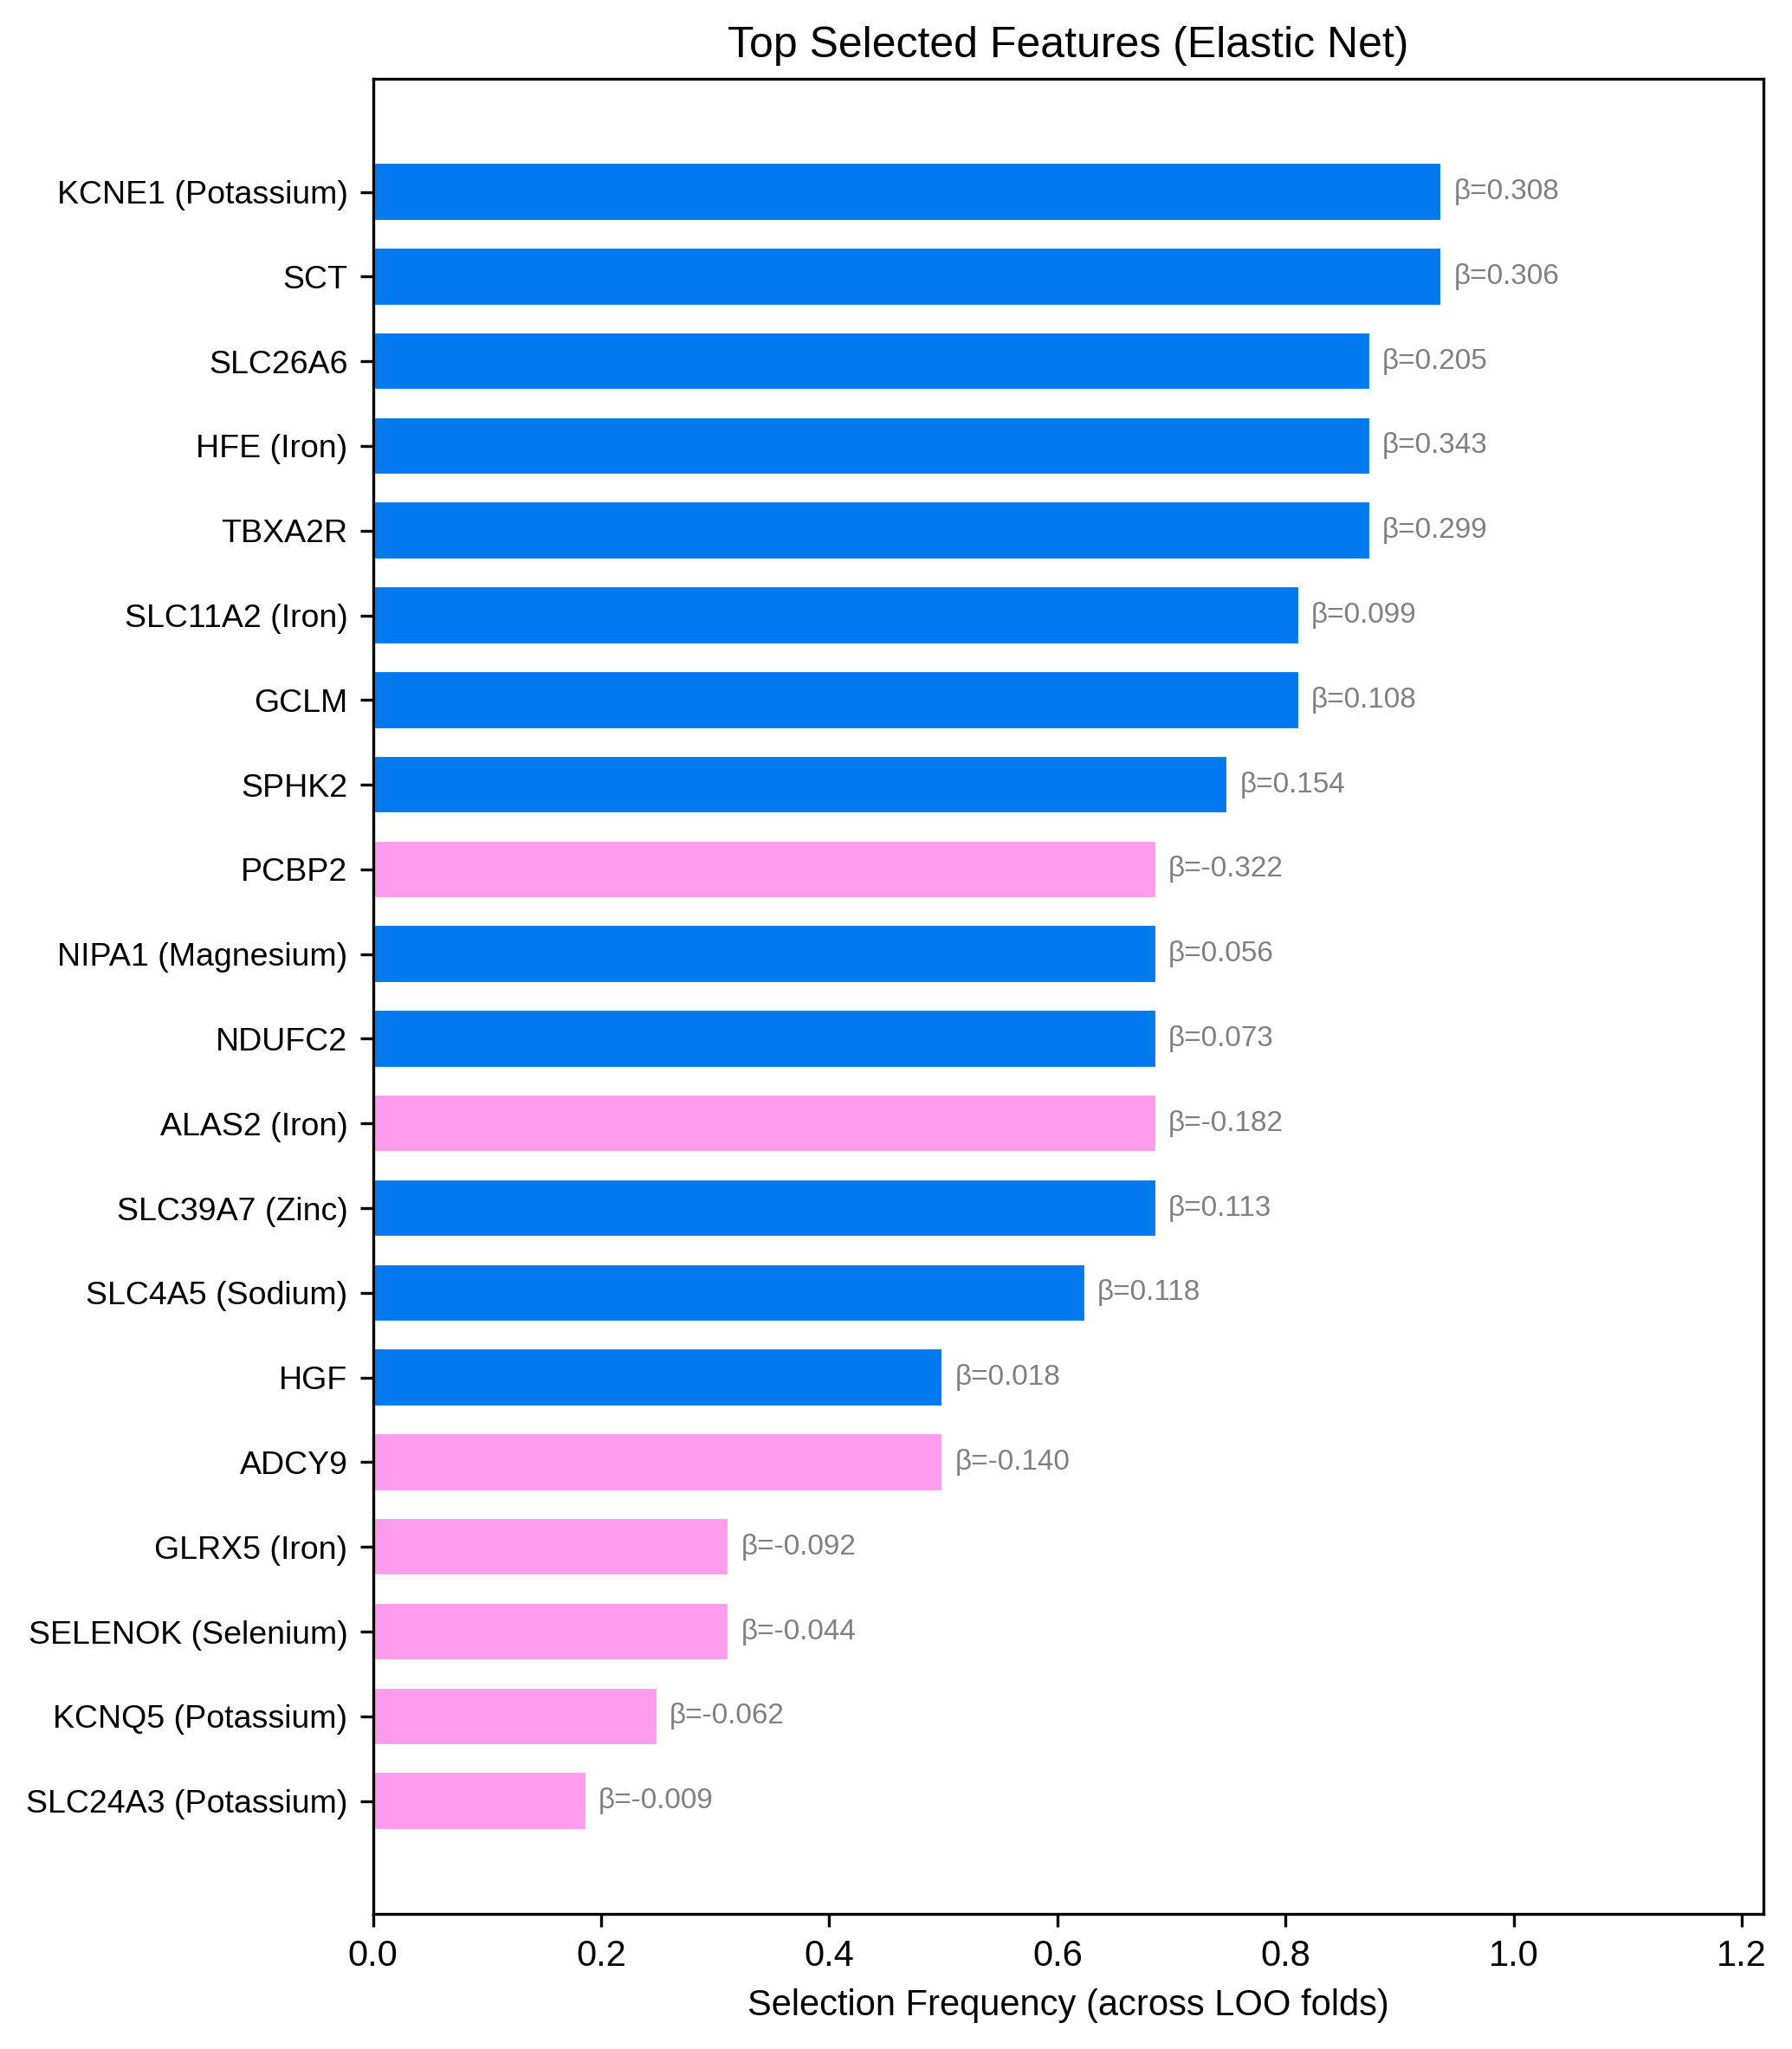
\includegraphics[width=\textwidth]{figures/figS8_selected_features.png}
\caption{}
\end{subfigure}

\vspace{0.5em}
\begin{subfigure}{0.48\textwidth}
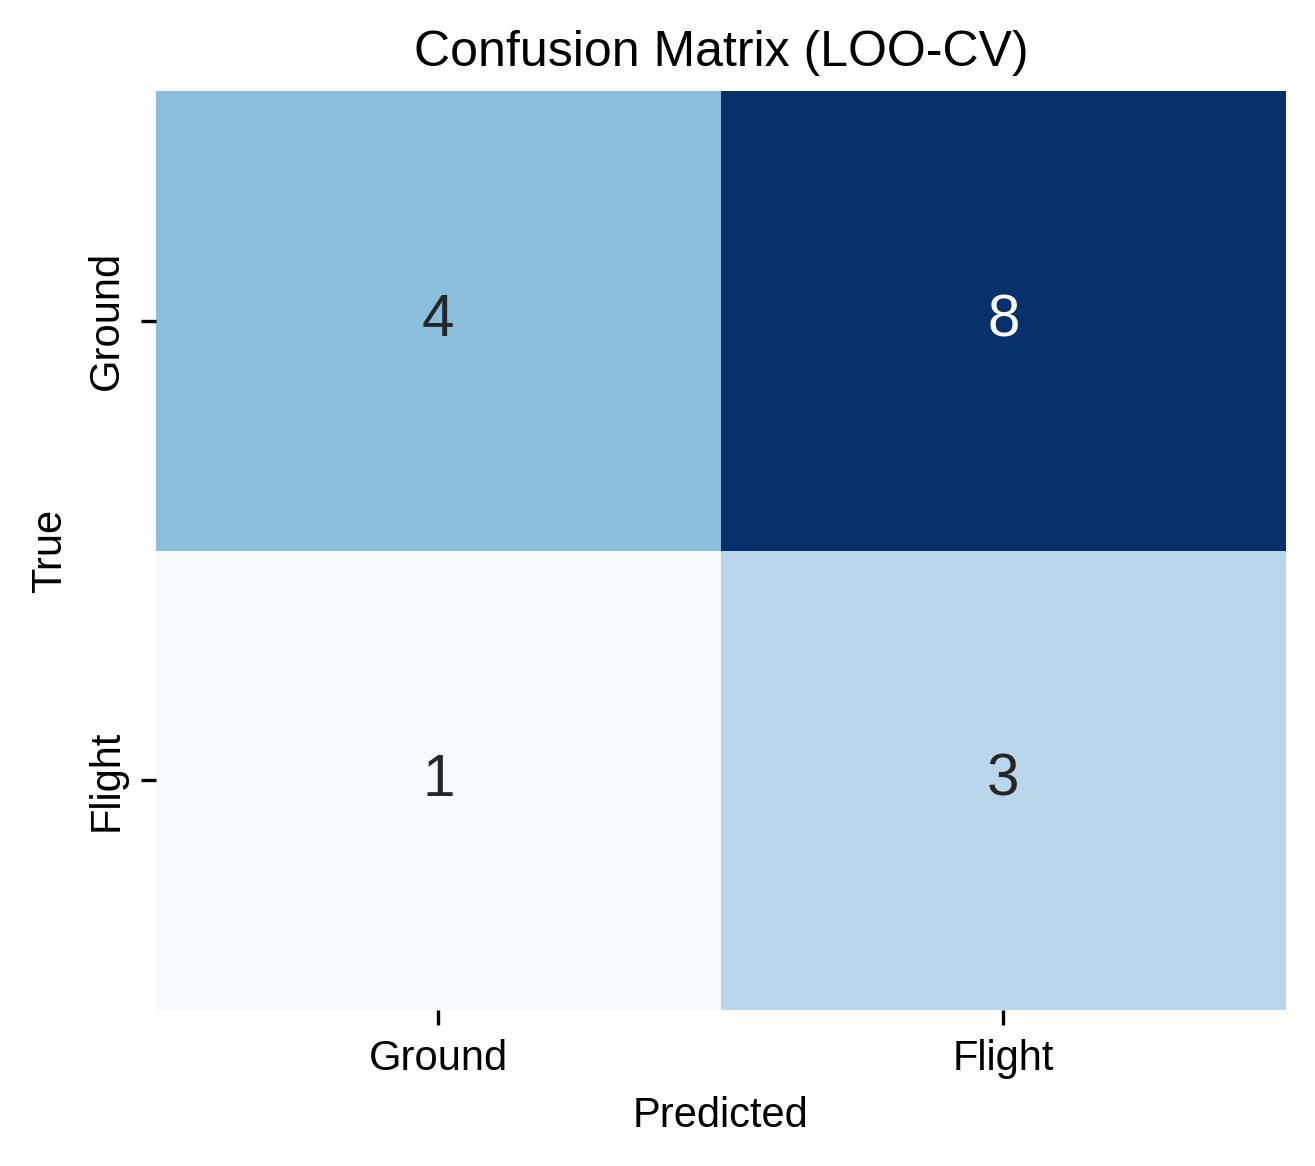
\includegraphics[width=\textwidth]{figures/figS7_confusion_matrix.png}
\caption{}
\end{subfigure}
\hfill
\begin{subfigure}{0.48\textwidth}
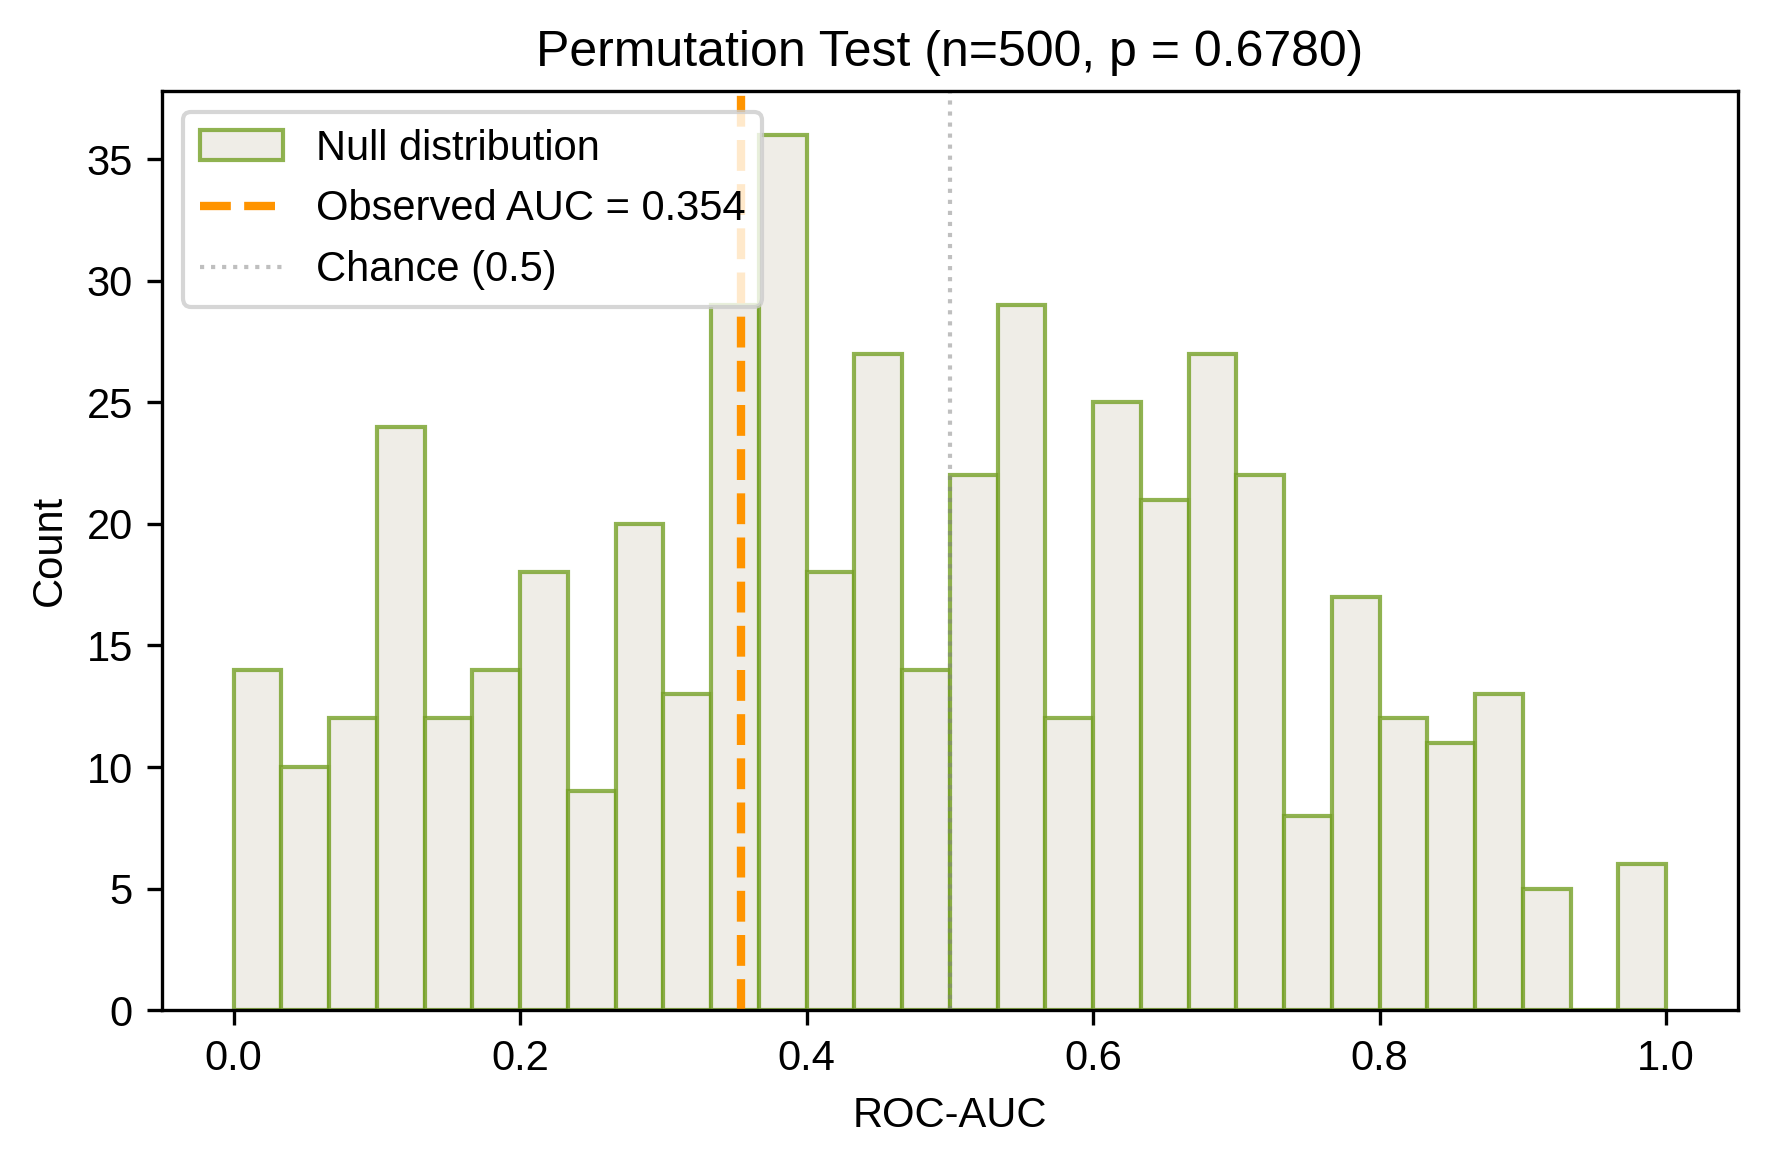
\includegraphics[width=\textwidth]{figures/figS6_permutation_null.png}
\caption{}
\end{subfigure}
\caption{Machine learning analysis. (a) Permutation importance for potassium (left) and sodium (right) regression under LOO-CV. Bar colors indicate the primary mineral association of each gene. (b) Stability-selected features from imbalance-aware elastic-net classification: selection frequency across LOO folds and mean coefficient magnitude, annotated with mineral pathway. (c) Confusion matrix for the best classification model (class-weighted elastic-net, LOO-CV). (d) Permutation null distribution for the classification AUC, with observed AUC marked.}
\label{fig:ml_results}
\end{figure}

\begin{table}[H]
\centering
\caption{Machine learning model comparison. Regression (v1): LOO-CV on top-200 variance genes. Classification (v2): nested LOO-CV on 784 mineral-pathway genes with class-weight balancing.}
\label{tab:ml_comparison}
\begin{tabular}{llrr}
\toprule
\textbf{Task} & \textbf{Model} & \textbf{Metric} & \textbf{Value} \\
\midrule
\multicolumn{4}{l}{\textit{Regression (LOO-CV, $n=16$)}} \\
Potassium & Ridge & $r$ / $R^2$ & 0.50 / 0.12 \\
Sodium & SVR-Linear & $r$ / $R^2$ & 0.46 / 0.19 \\
Hemoglobin & SVR-Linear & $r$ / $R^2$ & 0.48 / $-0.62$ \\
Calcium & Ridge & $r$ / $R^2$ & $-0.02$ / $-0.59$ \\
\midrule
\multicolumn{4}{l}{\textit{Classification (nested LOO-CV, 4 flight vs 12 ground)}} \\
SVM-RBF (balanced) & --- & AUC & 1.0 (null mean 0.121, $p < 0.002$) \\
ElasticNet (balanced) & --- & AUC & 0.10 ($p = 0.68$) \\
ElasticNet (filtered) & --- & AUC & 0.35 ($p = 0.68$) \\
Dummy (stratified) & --- & AUC & 0.50 \\
\bottomrule
\end{tabular}
\end{table}

\subsection{Cross-mission integration and deep learning analysis}

To increase astronaut sample size and test generalizability, we integrated per-sample RNA-seq from two independent spaceflight missions: the I4 cohort ($n = 4$ astronauts, 16 samples) and the Axiom-1 (AX-1) mission ($n = 2$ astronauts, 6 samples; GEO: GSE276490). Gene expression was harmonized to 779 common mineral-pathway genes, log$_2$-transformed, and batch-corrected by study-wise z-scoring. A denoising autoencoder (779 $\to$ 128 $\to$ 64 $\to$ 16-dimensional latent $\to$ 64 $\to$ 128 $\to$ 779; Gaussian noise $\sigma = 0.1$, dropout 0.3, $L_2$ weight decay $10^{-4}$) was trained with leave-one-astronaut-out (LOAO) cross-validation across all 6 astronauts (22 samples).

On the 16-dimensional latent space, a random forest classifier achieved a pooled LOAO AUC of 0.728 for flight vs.\ pre-flight discrimination ($p = 0.015$, 1000-permutation test; Figure~\ref{fig:dl_results}a--b), outperforming the same classifier on raw 779-dimensional expression (AUC = 0.621, $p = 0.167$). This demonstrates that the autoencoder's dimensionality reduction improves generalization in the extreme small-$n$ regime ($n = 6$ astronauts), where the raw feature space (779 genes) leads to overfitting. Other classifiers (logistic regression, SVM) performed near chance on both representations, consistent with the limited statistical power.

Regression on the latent space to predict serum mineral levels (I4 only, 4 astronauts) showed strong absolute correlations for hemoglobin (SVR-RBF, $|r| = 0.915$) and potassium (random forest, $|r| = 0.748$), though with negative sign --- an artifact of LOAO with $n = 4$ where models learn astronaut-specific patterns that reverse in held-out subjects (Figure~\ref{fig:dl_results}d). Sodium showed a positive correlation ($r = 0.431$). These results confirm that mineral-pathway latent features encode clinically relevant variation, but reliable individual-level prediction requires larger cohorts.

\begin{figure}[H]
\centering
\begin{subfigure}{0.48\textwidth}
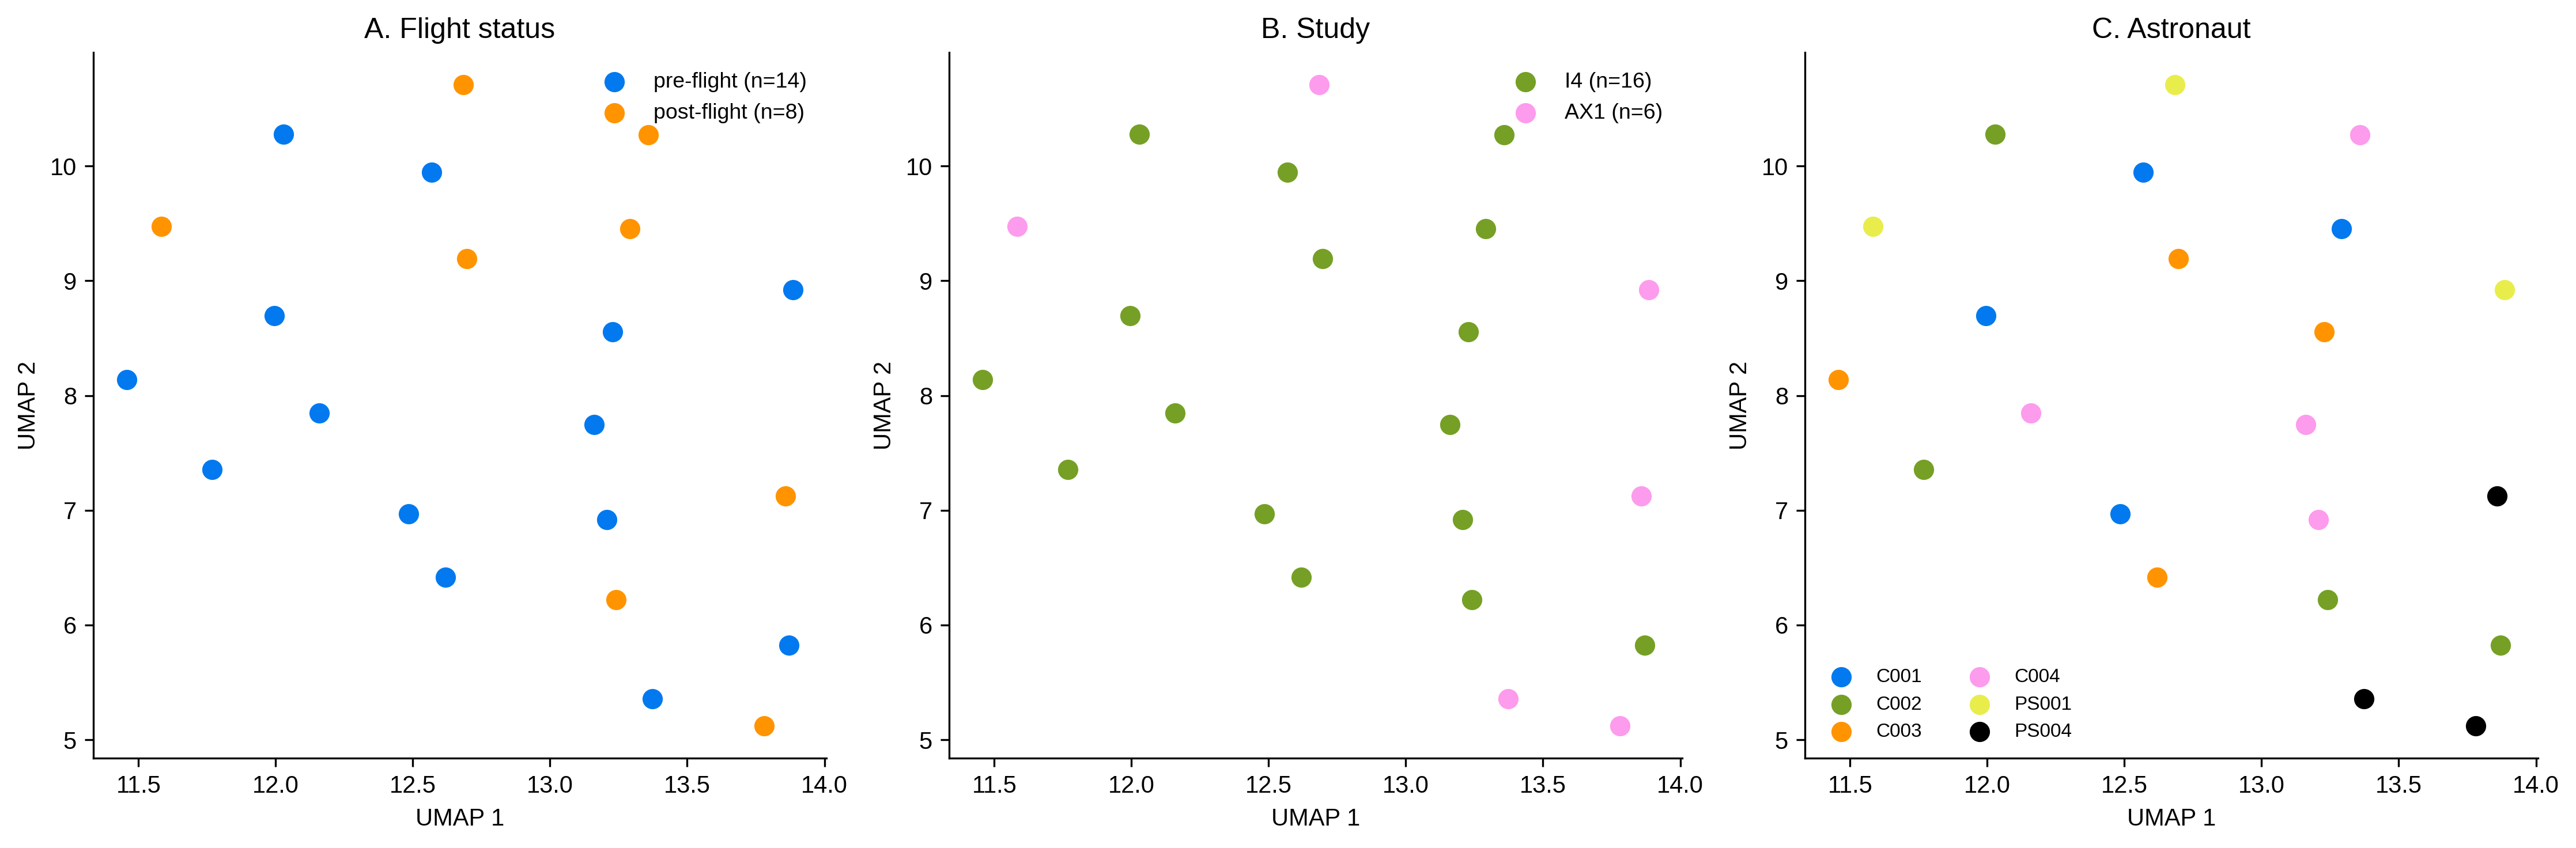
\includegraphics[width=\textwidth]{figures/dl_umap_latent.png}
\caption{}
\end{subfigure}
\hfill
\begin{subfigure}{0.48\textwidth}
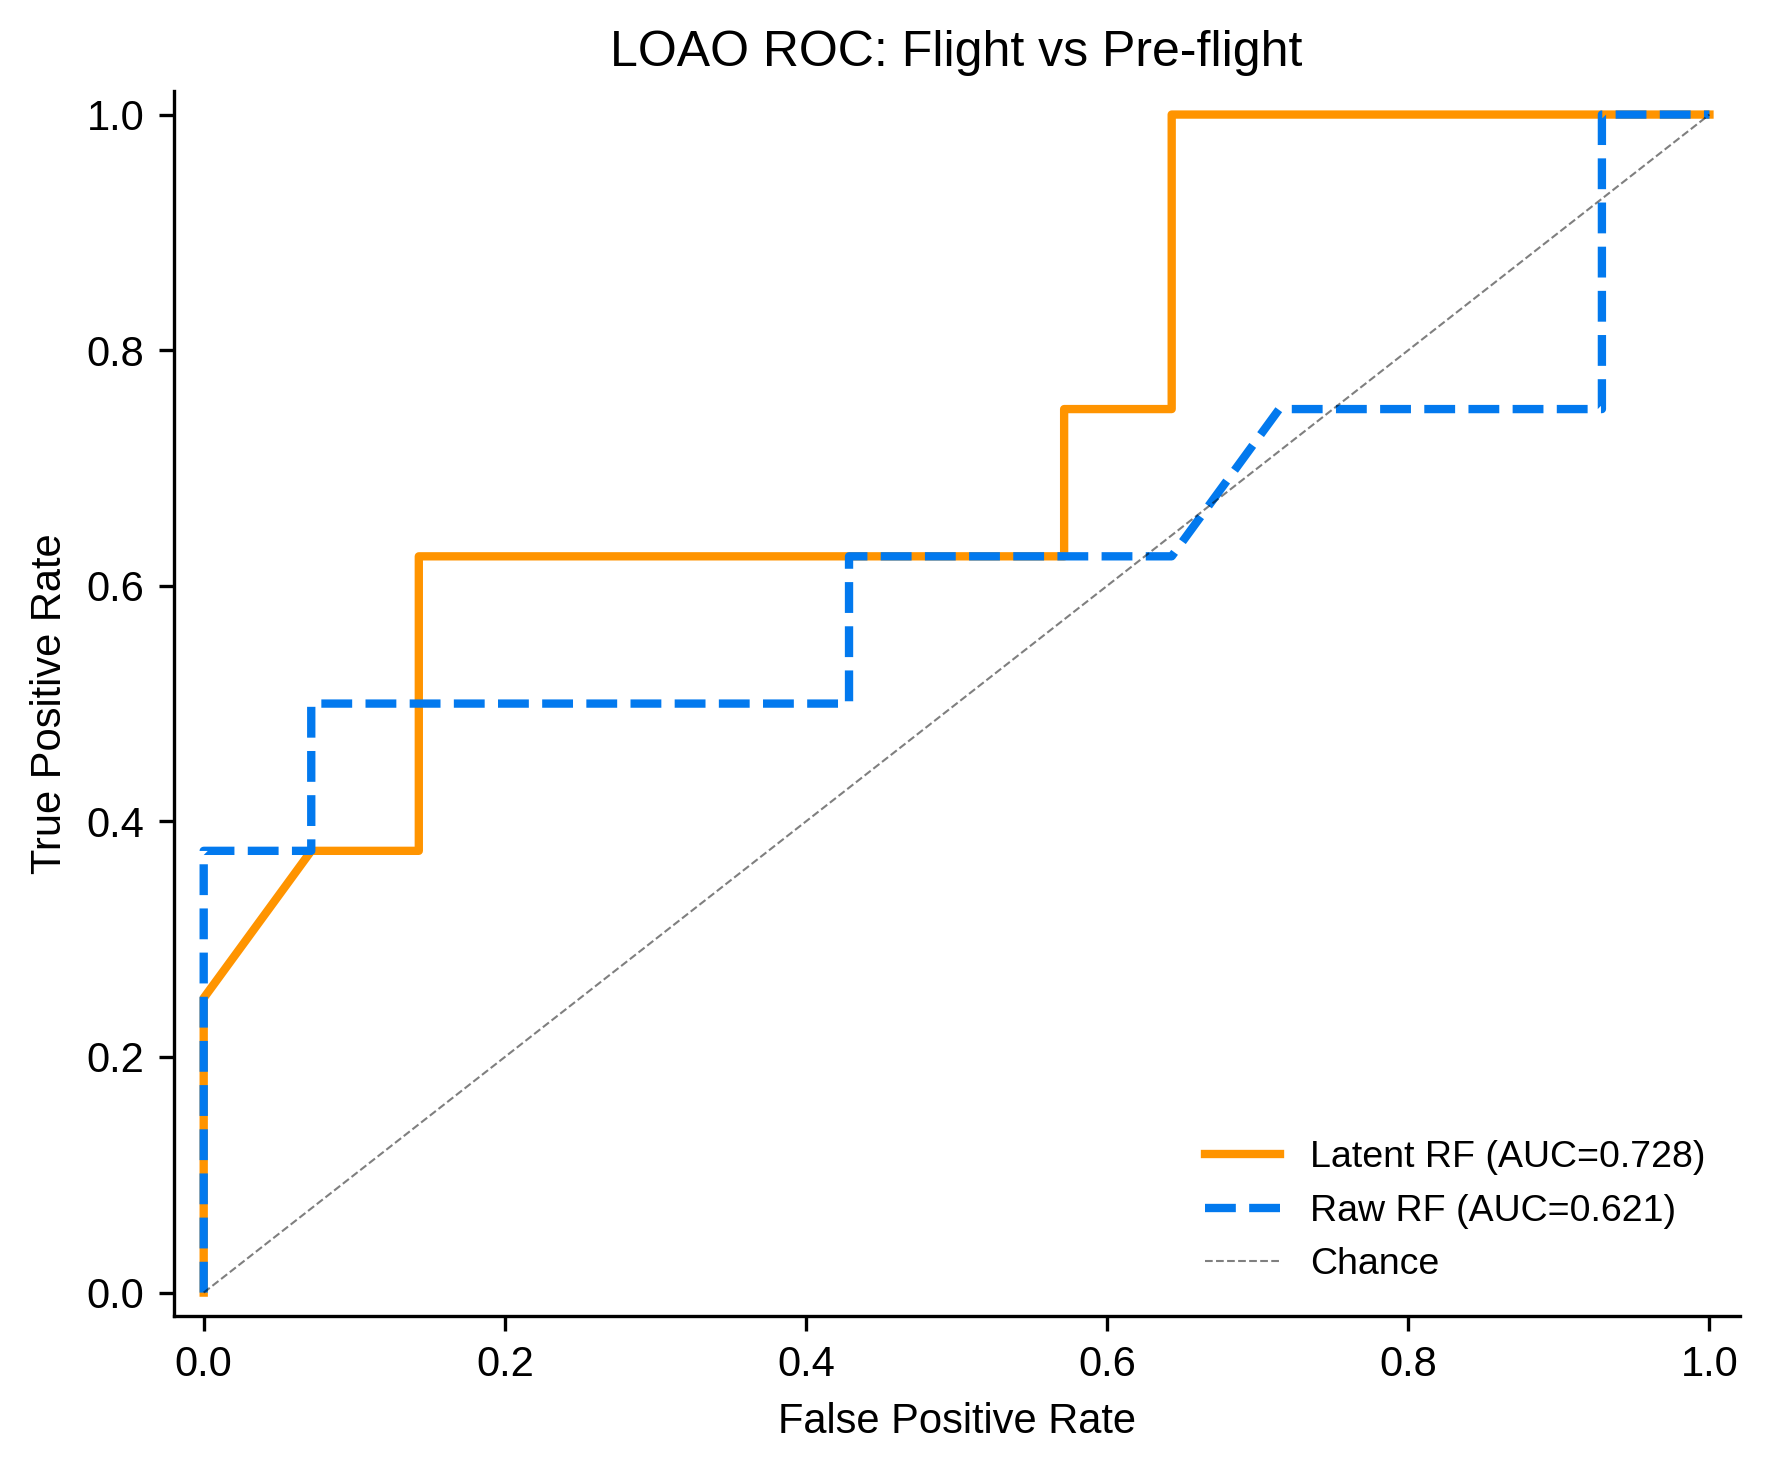
\includegraphics[width=\textwidth]{figures/dl_roc_curves.png}
\caption{}
\end{subfigure}

\vspace{0.5em}
\begin{subfigure}{0.48\textwidth}
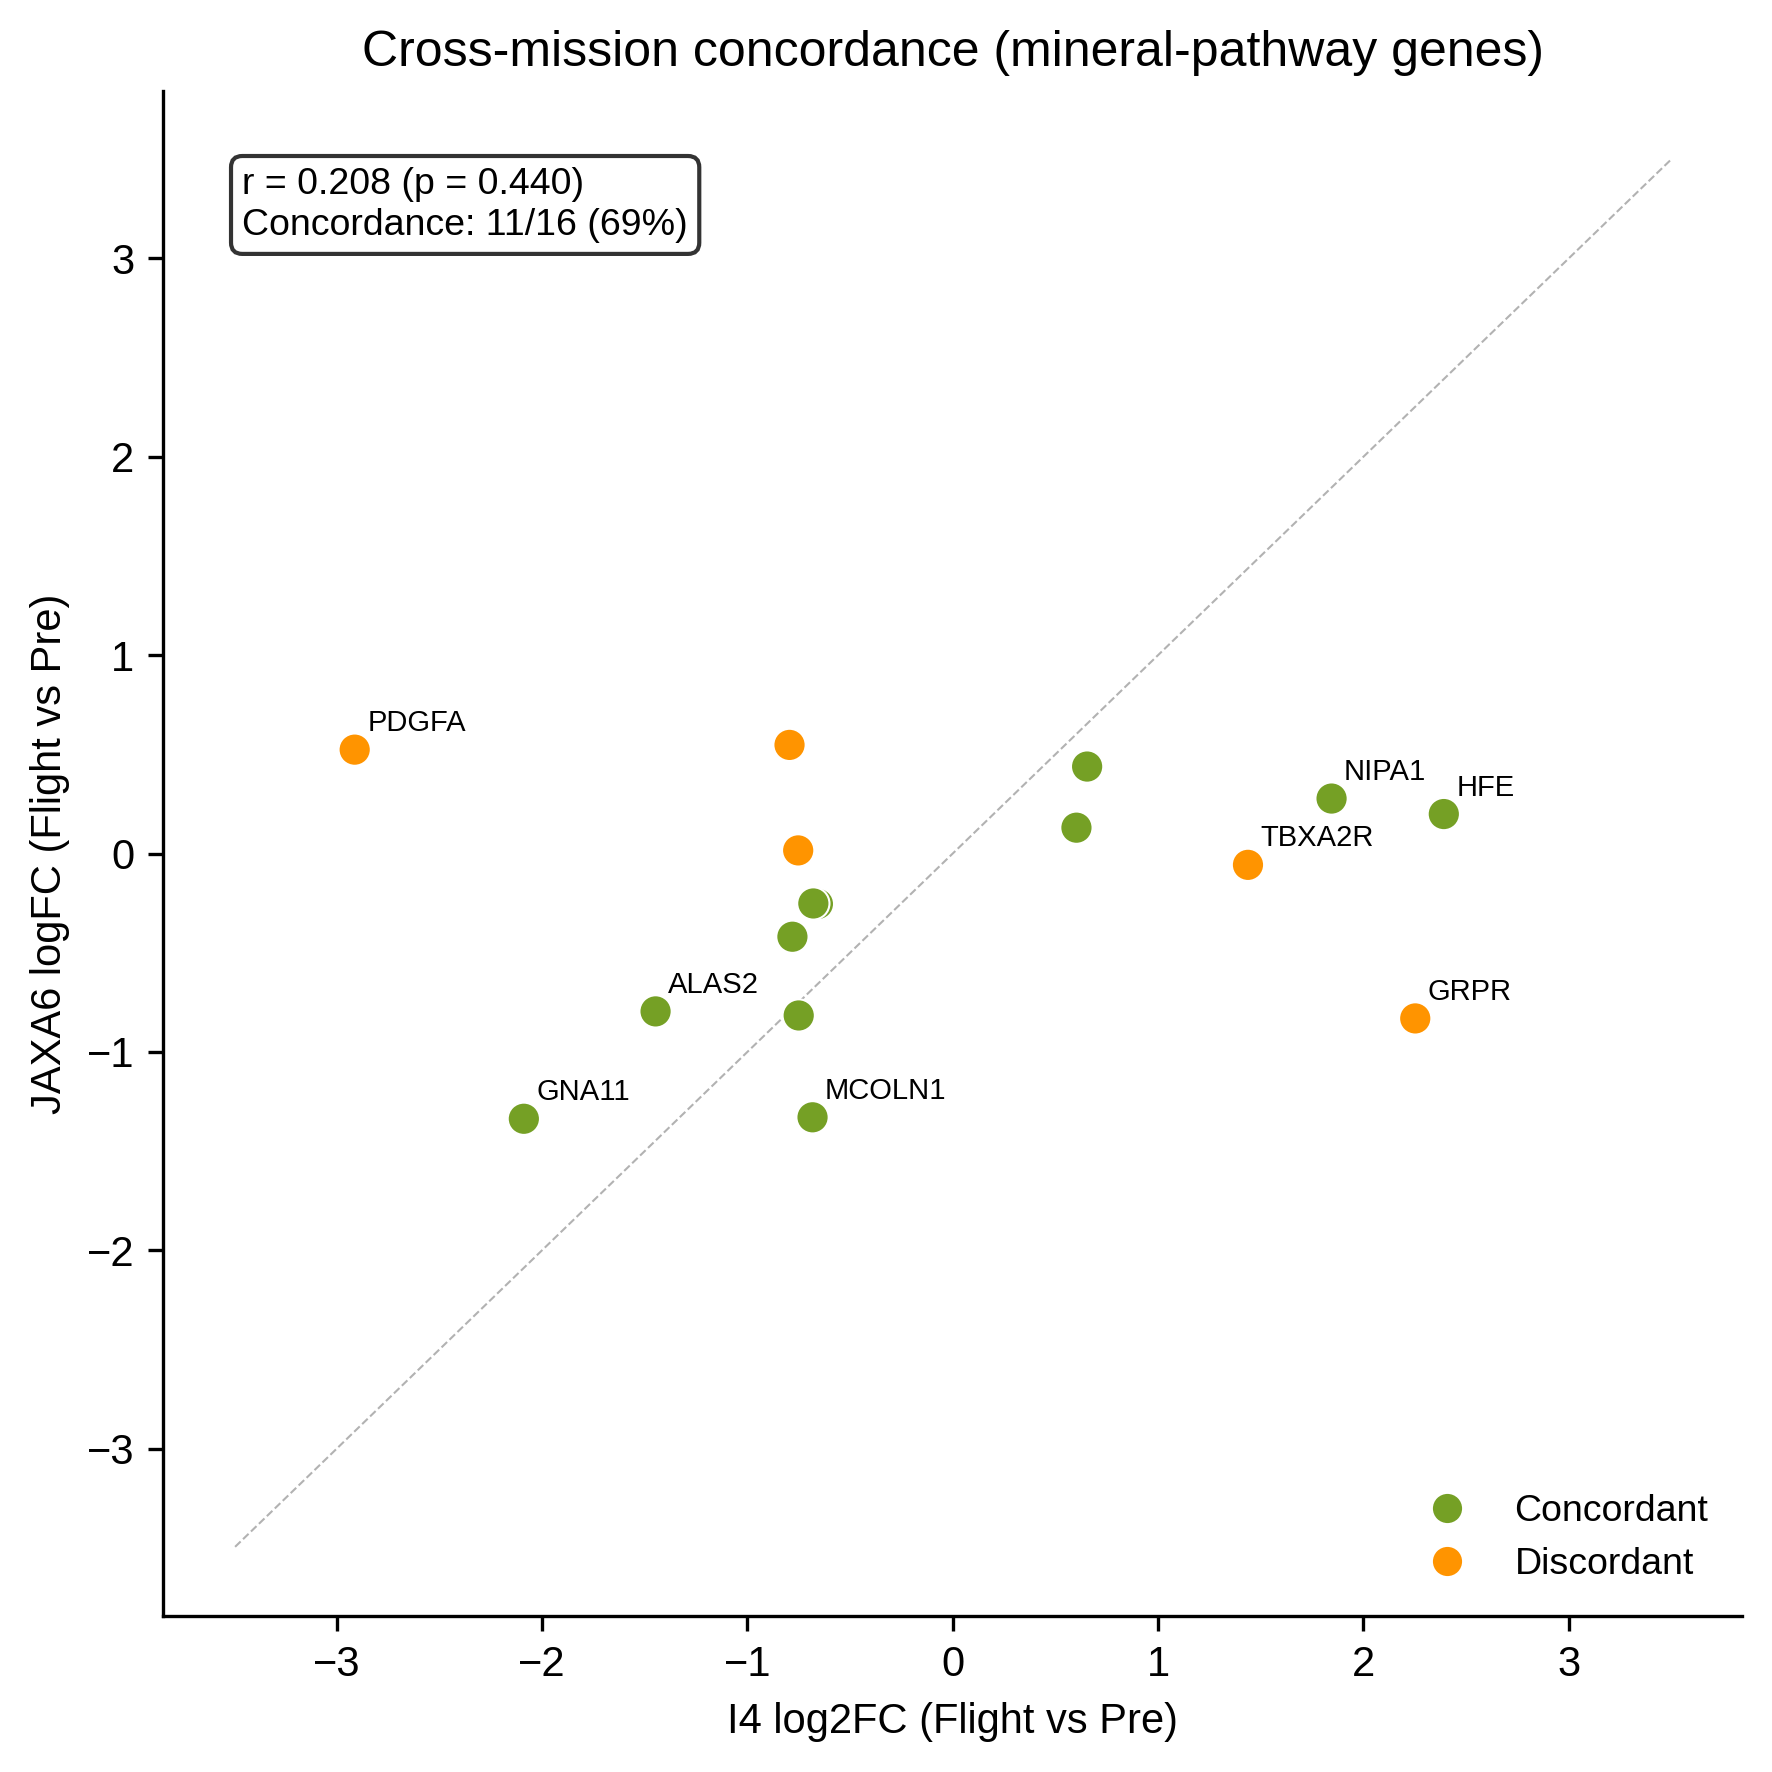
\includegraphics[width=\textwidth]{figures/dl_jaxa6_concordance.png}
\caption{}
\end{subfigure}
\hfill
\begin{subfigure}{0.48\textwidth}
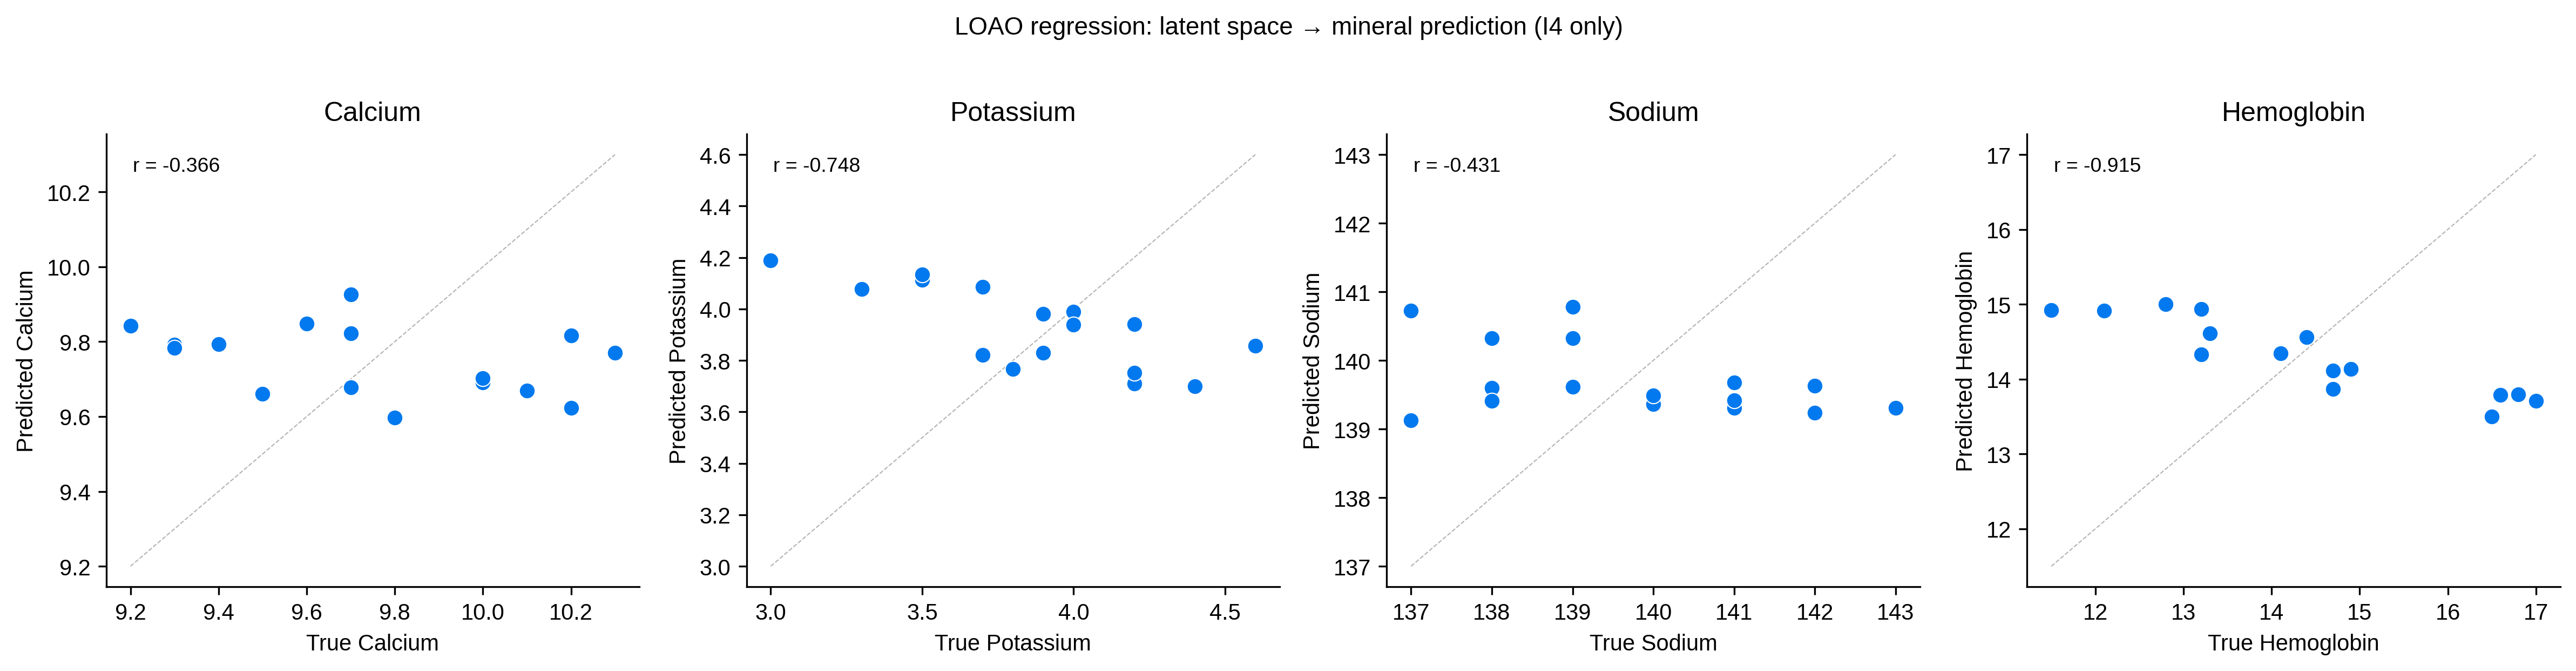
\includegraphics[width=\textwidth]{figures/dl_regression_scatter.png}
\caption{}
\end{subfigure}
\caption{Cross-mission integration and deep learning. (a) UMAP of the 16-dimensional autoencoder latent space (22 samples, 6 astronauts), colored by flight status, study, and astronaut identity. (b) LOAO ROC curves for flight vs.\ pre-flight classification: latent-space random forest (AUC = 0.728, $p = 0.015$) vs.\ raw-expression random forest (AUC = 0.621). (c) Cross-mission concordance: I4 vs.\ JAXA6 log$_2$FC for 16 overlapping mineral-pathway genes (68.8\% directional concordance). (d) LOAO regression scatter plots for calcium, potassium, sodium, and hemoglobin prediction from latent features (I4 only).}
\label{fig:dl_results}
\end{figure}

\subsubsection{JAXA6 cross-mission signature validation}

As an independent validation, we compared I4 flight-vs-pre differential expression against the JAXA6 mission (6 Japanese astronauts, plasma cell-free RNA-seq; OSD-530), which provides group-mean expression for 11 time points (3 pre-flight, 4 in-flight, 4 post-flight) but not per-sample data. Of the 20 I4 mineral-pathway DE genes (I4-FP1 comparison), 16 were present in the JAXA6 differential expression table. Directional concordance was 68.8\% (11/16 genes, binomial $p = 0.105$; Figure~\ref{fig:dl_results}c), with a weak positive log$_2$FC correlation ($r = 0.208$, $p = 0.44$). A weighted Stouffer meta-analysis (weighting by $\sqrt{n}$ per mission) identified one gene reaching FDR significance: \textit{ALAS2} (combined $p = 0.0016$, FDR $= 0.021$), downregulated during spaceflight in both I4 (log$_2$FC $= -1.45$) and JAXA6 (logFC $= -0.80$). ALAS2 encodes aminolevulinic acid synthase 2, the rate-limiting enzyme in erythroid heme biosynthesis, linking spaceflight-induced anemia to iron-pathway transcriptional suppression. Additionally, \textit{CNNM4} (a magnesium transporter selected by ML stability selection) was independently significant in JAXA6 (logFC $= -2.09$, adj-$P = 0.045$), providing cross-mission validation of an ML-identified biomarker.

\subsubsection{Architecture comparison: VAE and FT-Transformer}

To test whether the DAE's classification advantage generalizes to alternative deep learning architectures, we trained two additional models on the same 779-gene, 22-sample dataset under identical LOAO cross-validation:

\textit{Variational autoencoder (VAE).} A $\beta$-VAE with architecture 779 $\to$ 128 $\to$ 64 $\to$ 16 (mean and log-variance) $\to$ 64 $\to$ 128 $\to$ 779, trained with $\beta = 0.5$, dropout 0.3, $L_2$ weight decay $10^{-4}$, and the same Adam optimizer (lr $= 10^{-3}$, 300 epochs, patience 30). The KL regularization encourages a smooth latent manifold but may over-compress in the small-$n$ regime.

\textit{FT-Transformer.} A lightweight feature-tokenizer transformer treating each gene as a token with a value embedding (16-dim) and a learned gene-identity embedding (779 $\times$ 16). A single transformer encoder layer (4 heads, FFN dimension 32, pre-LN, GELU) processes the 779 tokens, and a CLS token aggregates to a 16-dimensional latent. Heavy regularization (dropout 0.5, $L_2$ $10^{-3}$, gradient clipping at norm 1.0) was applied. The model has 117,707 parameters and was trained for 150 epochs (patience 20, lr $= 5 \times 10^{-4}$).

\textit{Multi-omics consensus baseline.} Since per-sample proteomics was not available in OSDR (OSD-581 is a Mars simulation, not I4), we constructed a 15-gene multi-omics consensus set from the intersection of RNA-seq mineral-pathway genes and proteomics DE genes ($p < 0.05$ in I4-FP1 or I4-FP2). This 15-gene set (APP, ATP6AP1, ATP6V0D1, CYBB, FXYD2, GCLM, GPX1, LOX, LOXL1, PDGFA, S100A11, S100A12, S100A8, S100A9, SOD3) was used as a direct classification baseline without autoencoder encoding.

\textit{Classification results.} The DAE + random forest combination remained the best overall classifier (AUC = 0.728, $p = 0.015$; Figure~\ref{fig:dl_extended}a--b). The FT-Transformer achieved significant classification with a different optimal classifier --- SVM-RBF (AUC = 0.661, $p = 0.006$) --- suggesting that the transformer's attention-based latent space has different geometric properties than the DAE's reconstruction-based latent. The VAE did not reach significance (best: RF, AUC = 0.621, $p = 0.143$), consistent with the hypothesis that KL regularization over-compresses the latent space when $n = 6$ astronauts. Raw 779-dimensional expression (AUC = 0.621, $p = 0.176$) and the 15-gene multi-omics consensus (AUC = 0.598, $p = 0.168$) both failed to reach significance, confirming that dimensionality reduction is essential in this regime.

\textit{Regression results.} All architectures produced strong absolute correlations for hemoglobin prediction (DAE: $|r| = 0.915$, $p = 0.05$; VAE: $|r| = 0.930$, $p < 0.01$; Transformer: $|r| = 0.929$; Figure~\ref{fig:dl_extended}c). The VAE + SVR-linear combination was the only regression reaching permutation significance ($r = -0.930$, $p < 0.01$), though the negative sign reflects the LOAO artifact with $n = 4$ astronauts. Potassium prediction was strongest for the Transformer ($|r| = 0.801$, $p = 0.06$). These results confirm that all three architectures encode clinically relevant mineral variation, but the small sample size limits reliable individual-level prediction.

\textit{Ensemble analysis.} To test whether the DAE and FT-Transformer encode complementary information, we evaluated two ensemble strategies (Figure~\ref{fig:dl_extended}a--b). A concatenation ensemble (32-dimensional DAE+Transformer features) with random forest achieved AUC = 0.692 ($p = 0.024$) --- significant but lower than the DAE alone (0.728), suggesting that the expanded feature space introduces noise in the small-$n$ regime. In contrast, a prediction-level averaging ensemble (mean of DAE+RF and Transformer+SVM-RBF probabilities) achieved the highest AUC of any configuration: 0.750 ($p = 0.008$), surpassing both individual architectures. This demonstrates that the two architectures capture partially independent flight-status signals --- the DAE's reconstruction-based latent and the Transformer's attention-based latent encode complementary structure that is lost when merged at the feature level but preserved when combined at the decision level.

The latent space correlation analysis (Figure~\ref{fig:dl_extended}e) confirms this complementarity: pairwise correlations between DAE, VAE, and Transformer latent dimensions are generally weak ($|r| < 0.5$ for most dimension pairs), indicating that each architecture discovers different projections of the 779-gene space. The per-astronaut AUC breakdown (Figure~\ref{fig:dl_extended}f) reveals that the ensemble's improvement is driven by better classification of AX-1 astronauts (PS001, PS004), where the averaging ensemble achieves perfect AUC (1.0) compared to 0.67--1.0 for individual architectures.

\begin{figure}[H]
\centering
\begin{subfigure}{0.32\textwidth}
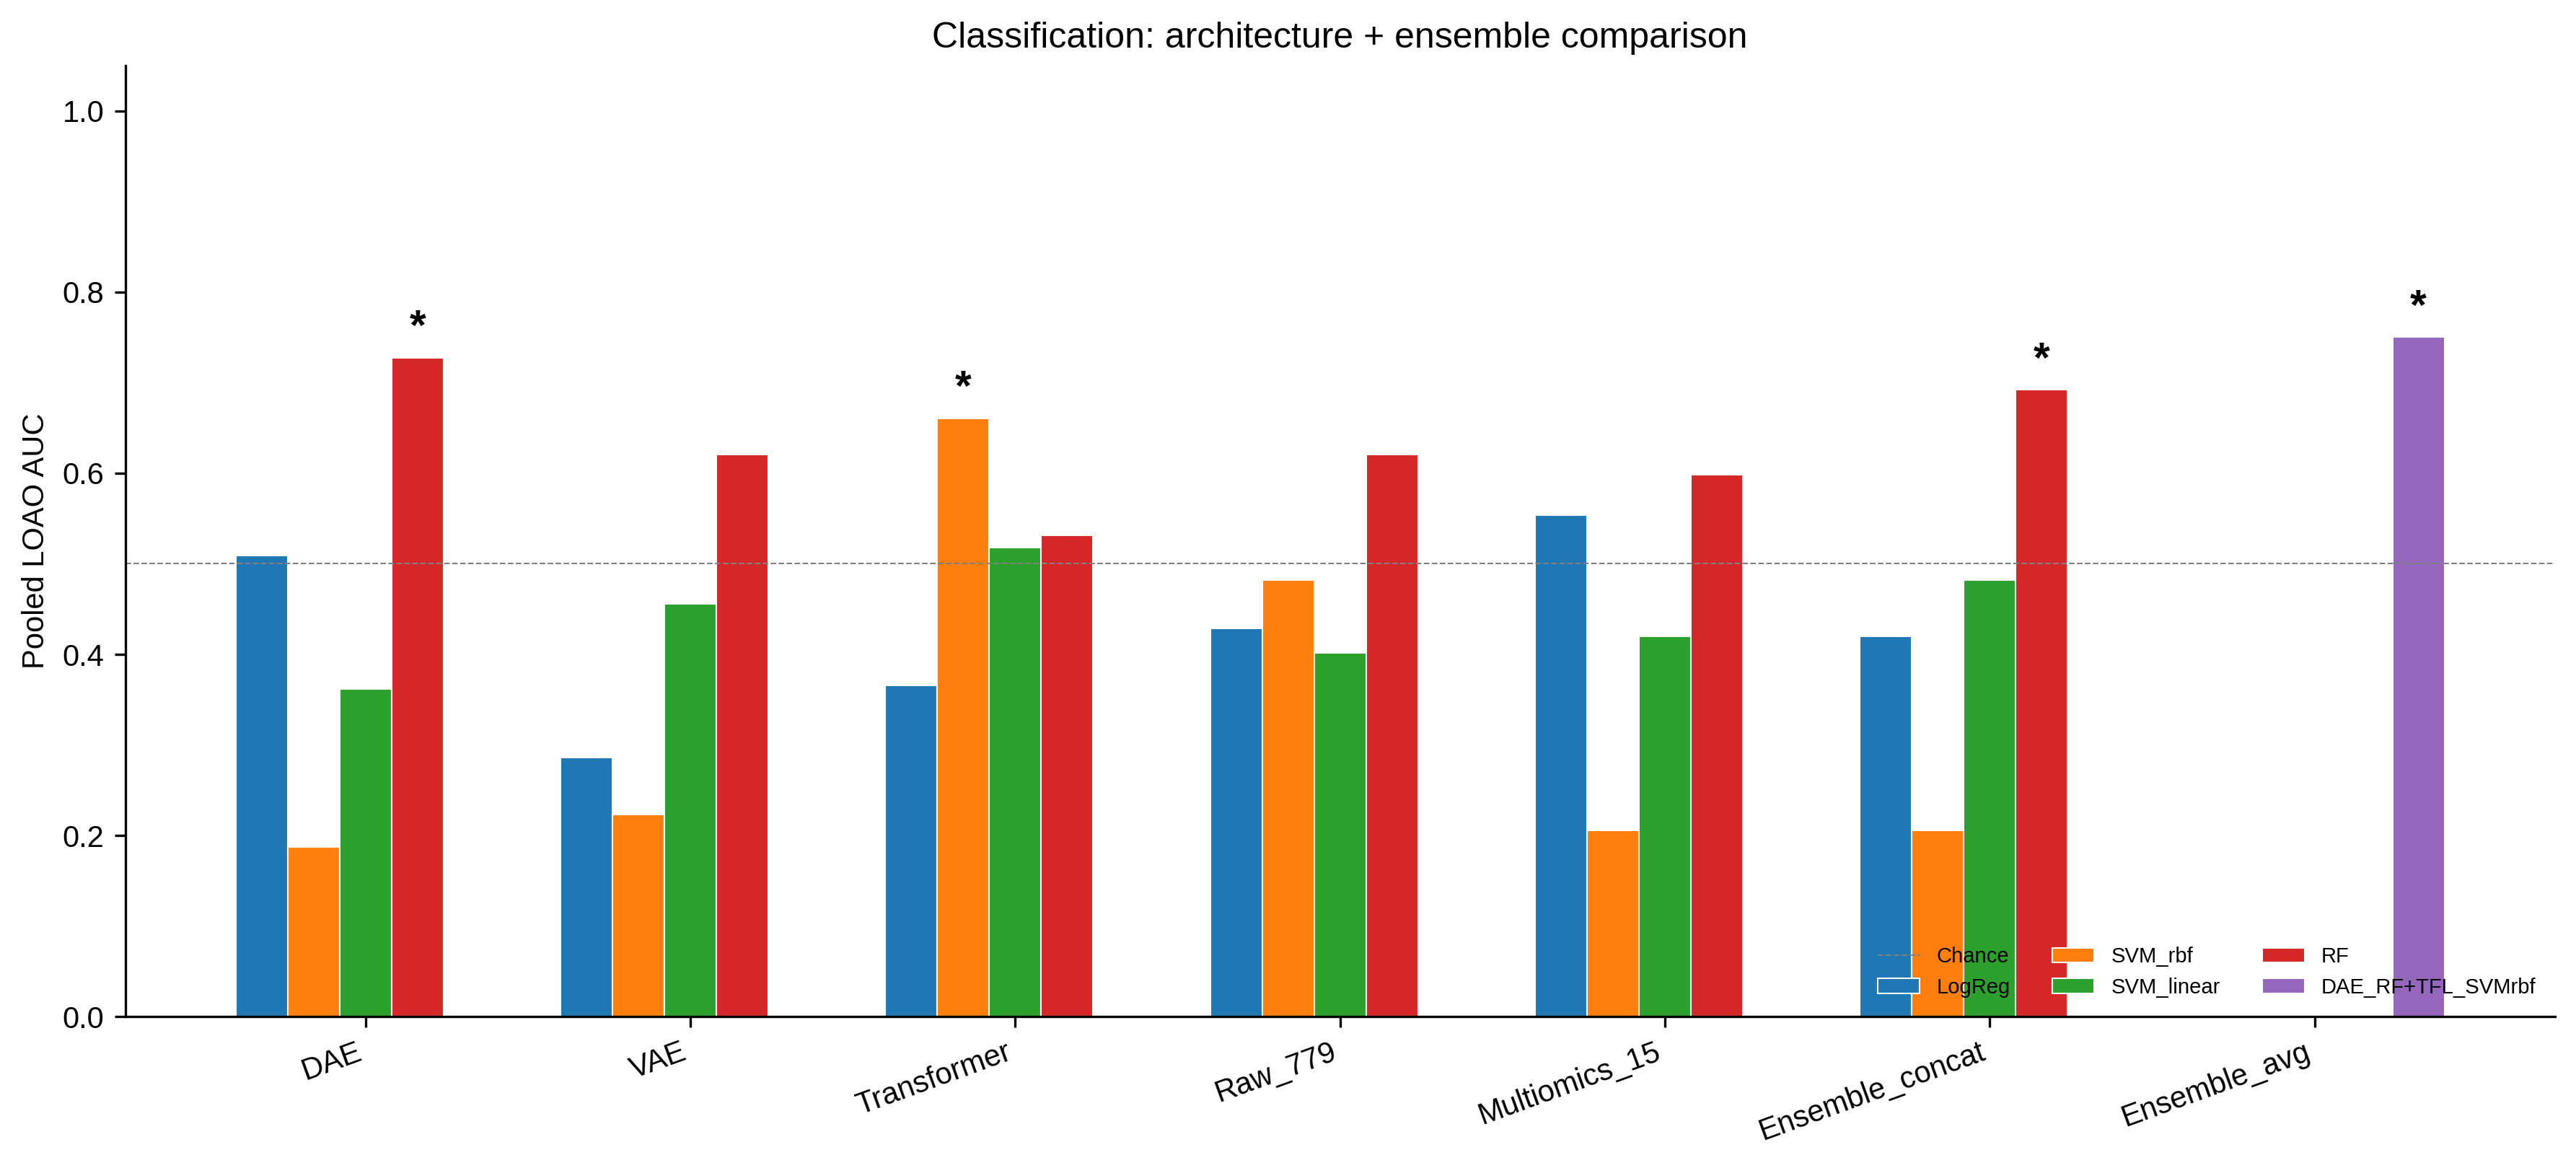
\includegraphics[width=\textwidth]{figures/dl_extended_auc_comparison.png}
\caption{}
\end{subfigure}
\hfill
\begin{subfigure}{0.32\textwidth}
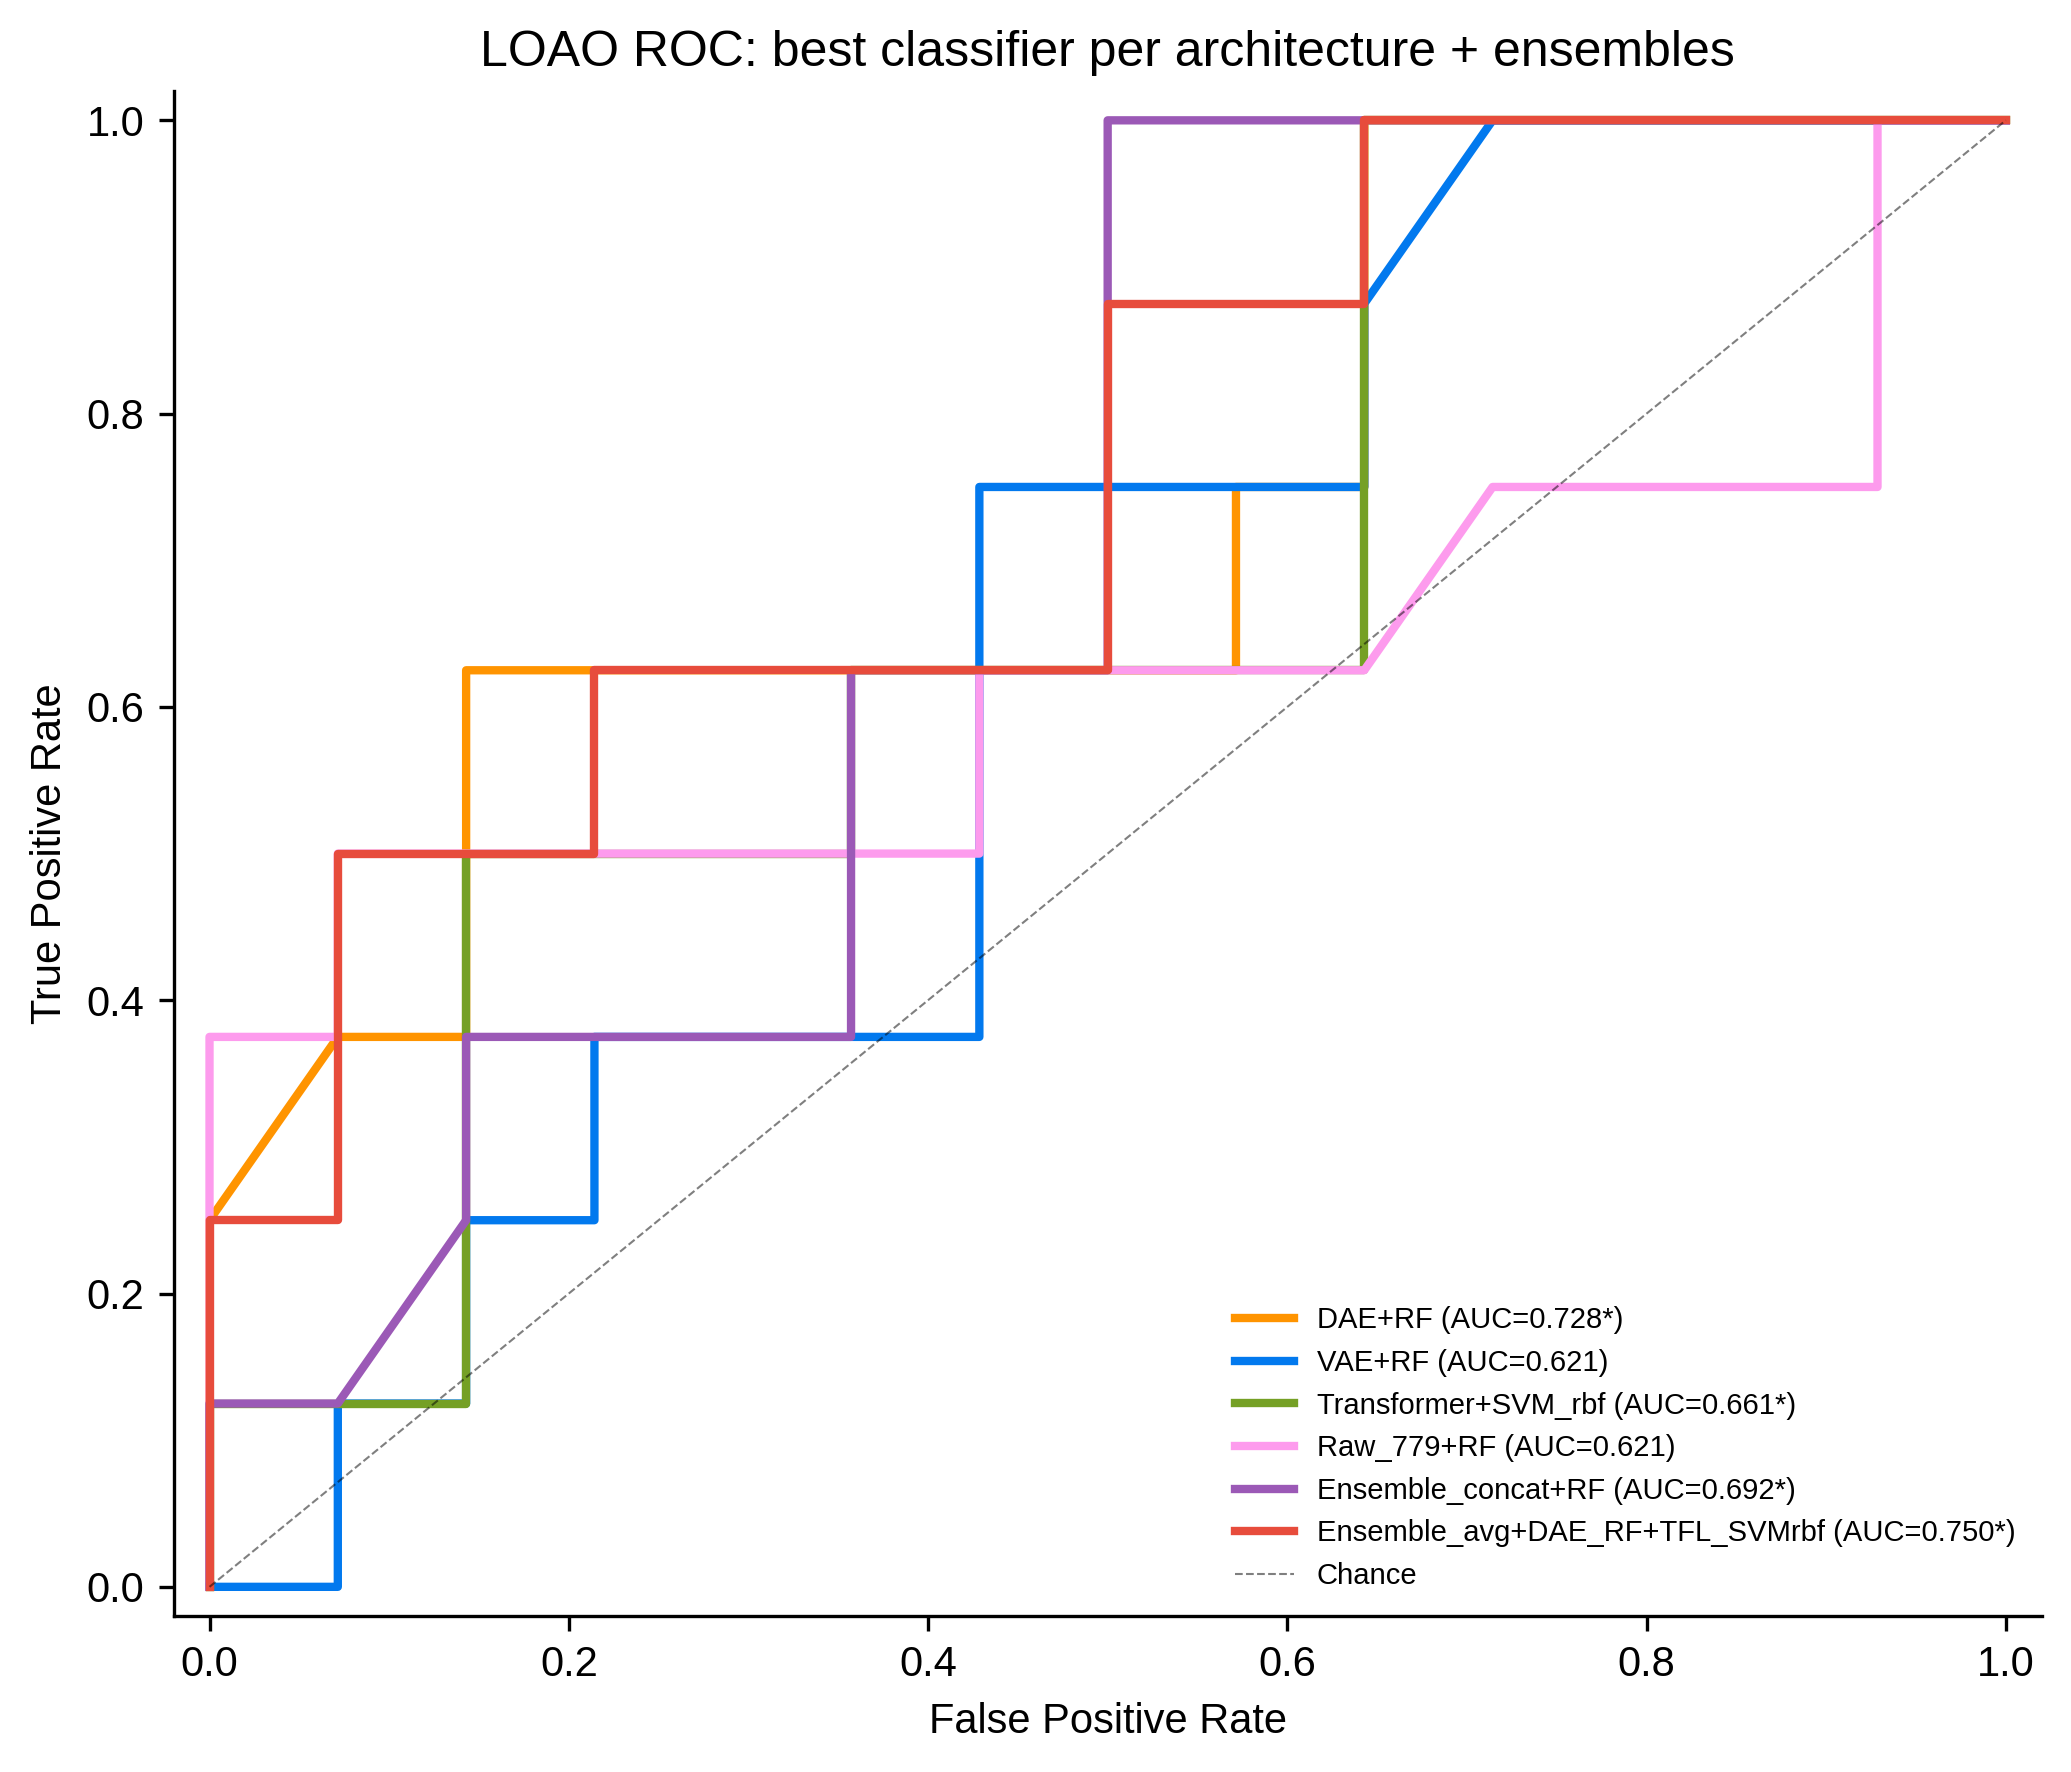
\includegraphics[width=\textwidth]{figures/dl_extended_roc_overlay.png}
\caption{}
\end{subfigure}
\hfill
\begin{subfigure}{0.32\textwidth}
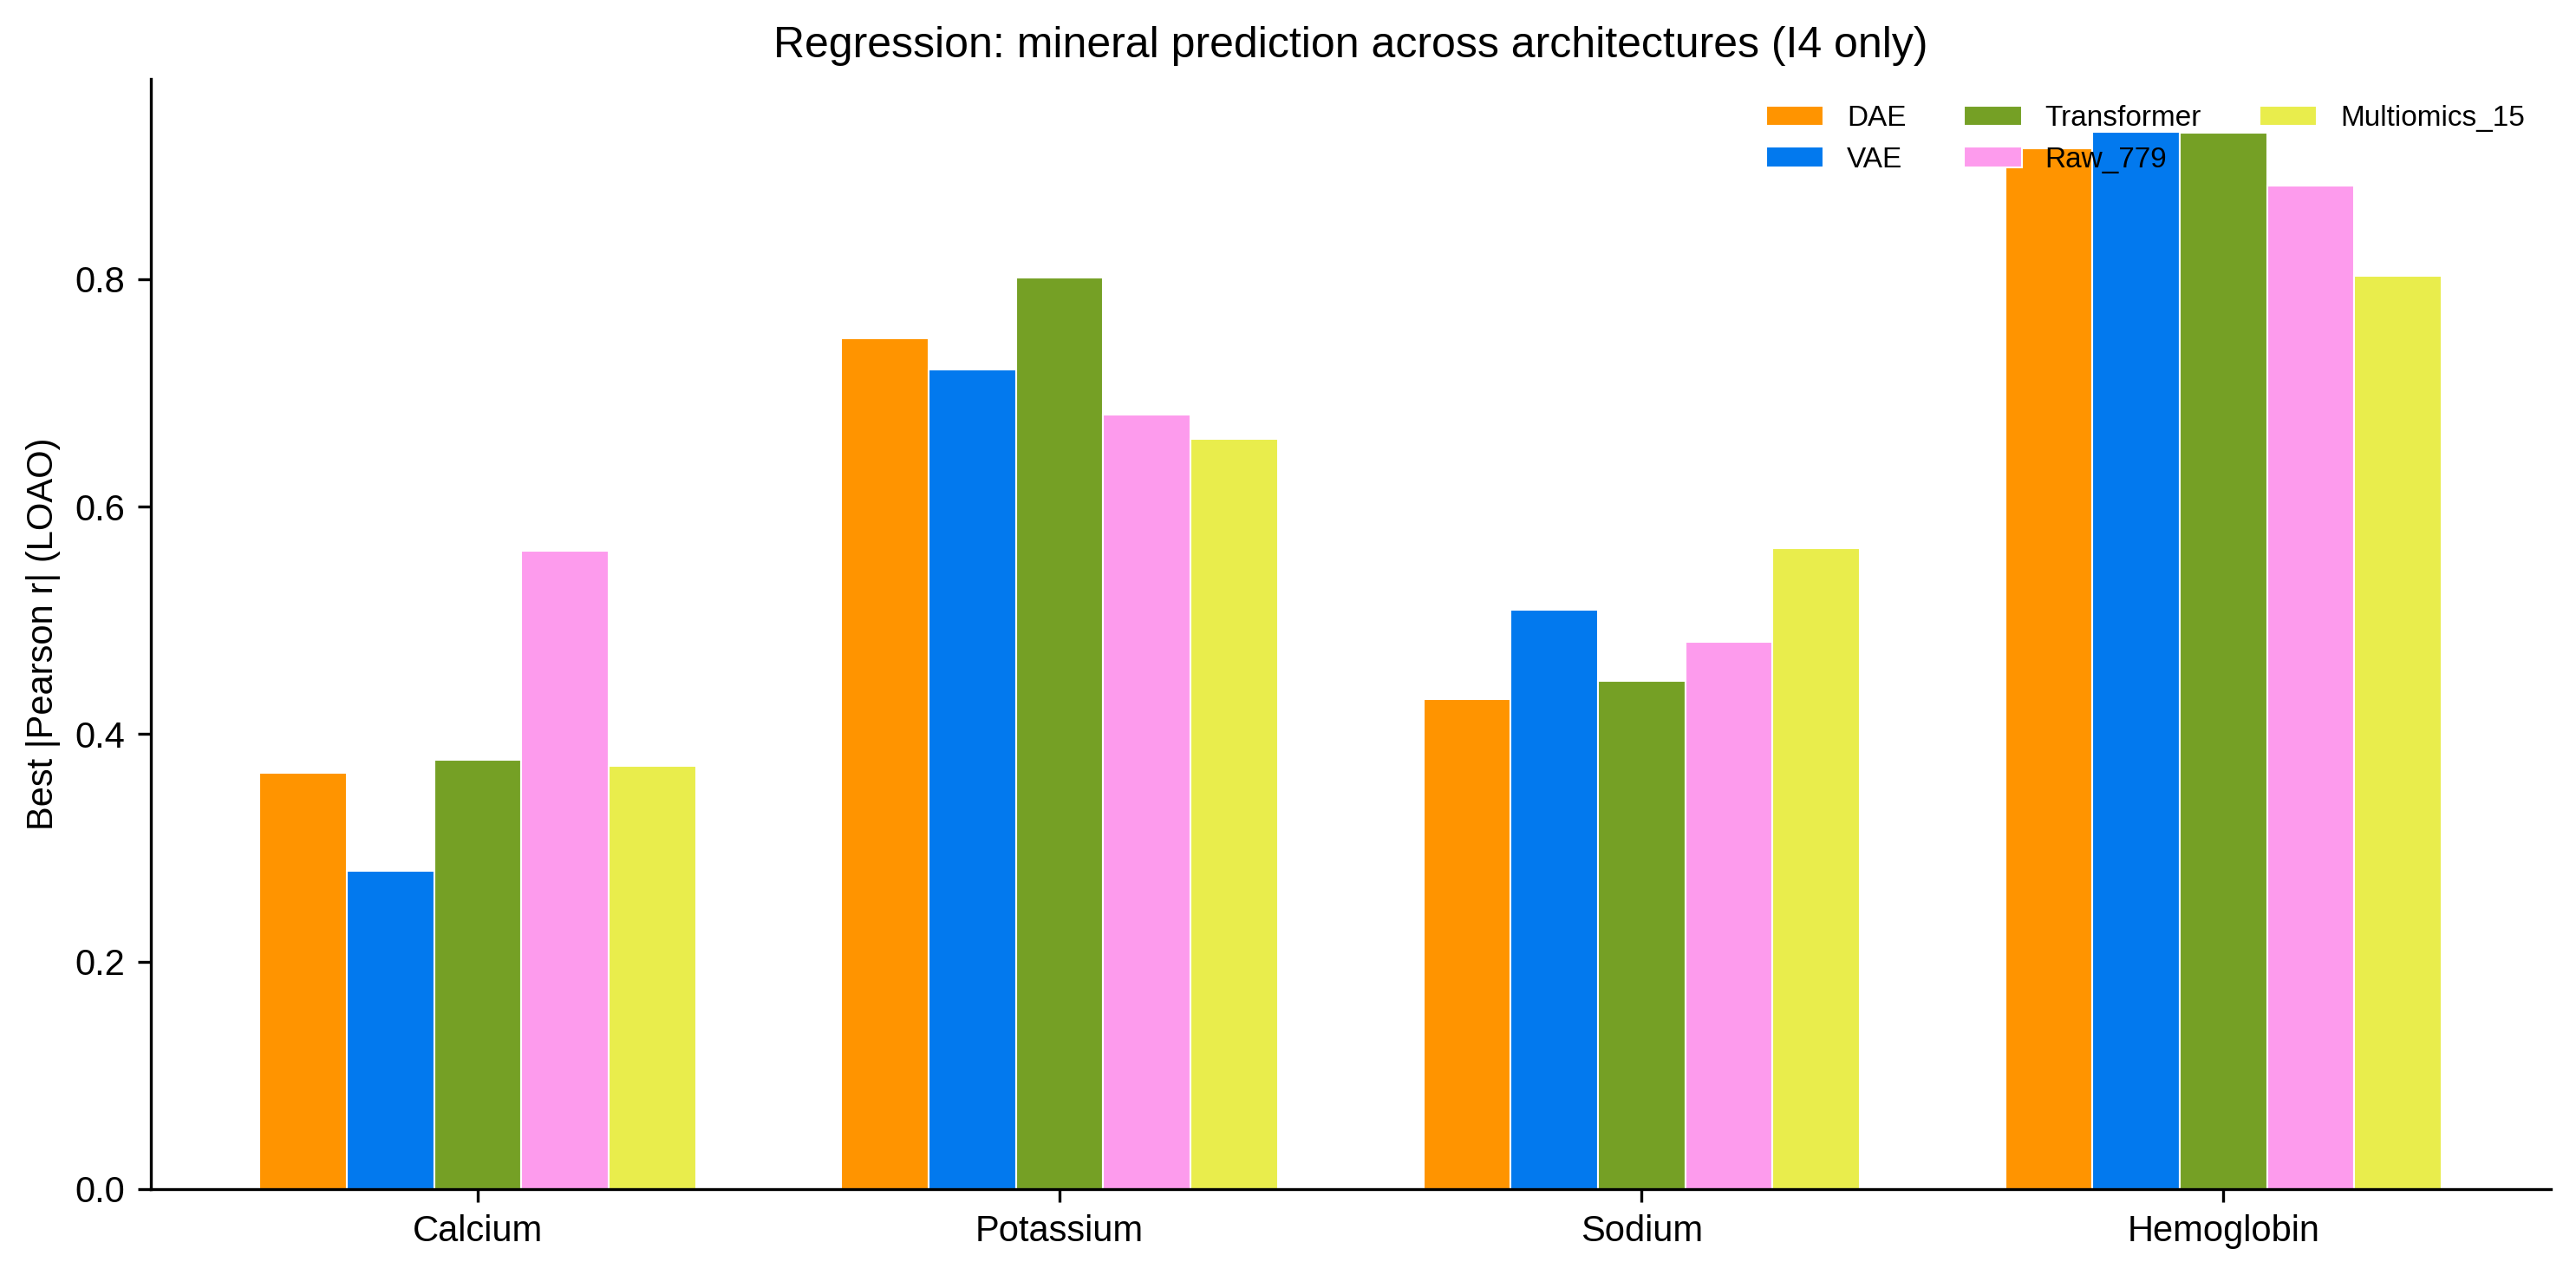
\includegraphics[width=\textwidth]{figures/dl_extended_regression_comparison.png}
\caption{}
\end{subfigure}

\vspace{0.5em}
\begin{subfigure}{0.32\textwidth}
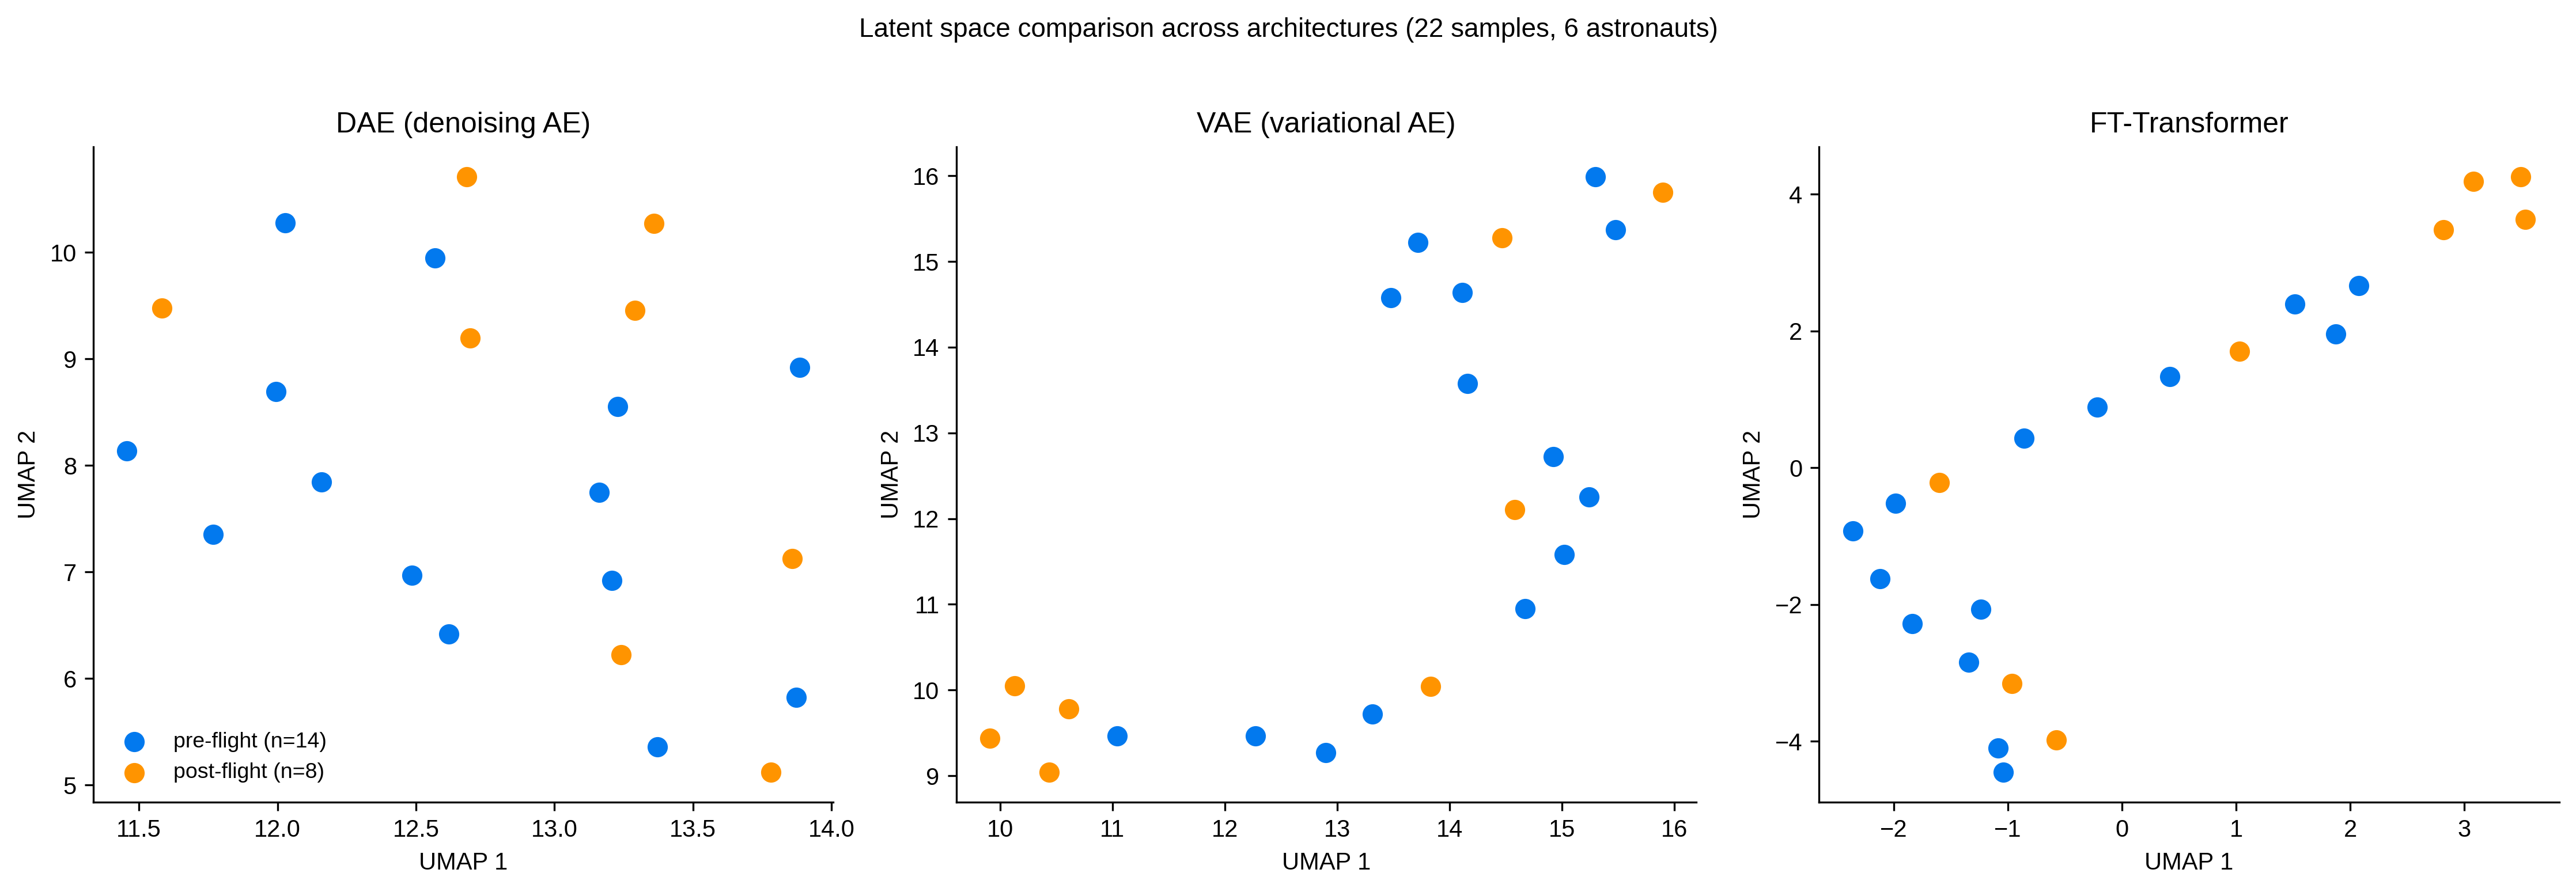
\includegraphics[width=\textwidth]{figures/dl_extended_umap_comparison.png}
\caption{}
\end{subfigure}
\hfill
\begin{subfigure}{0.32\textwidth}
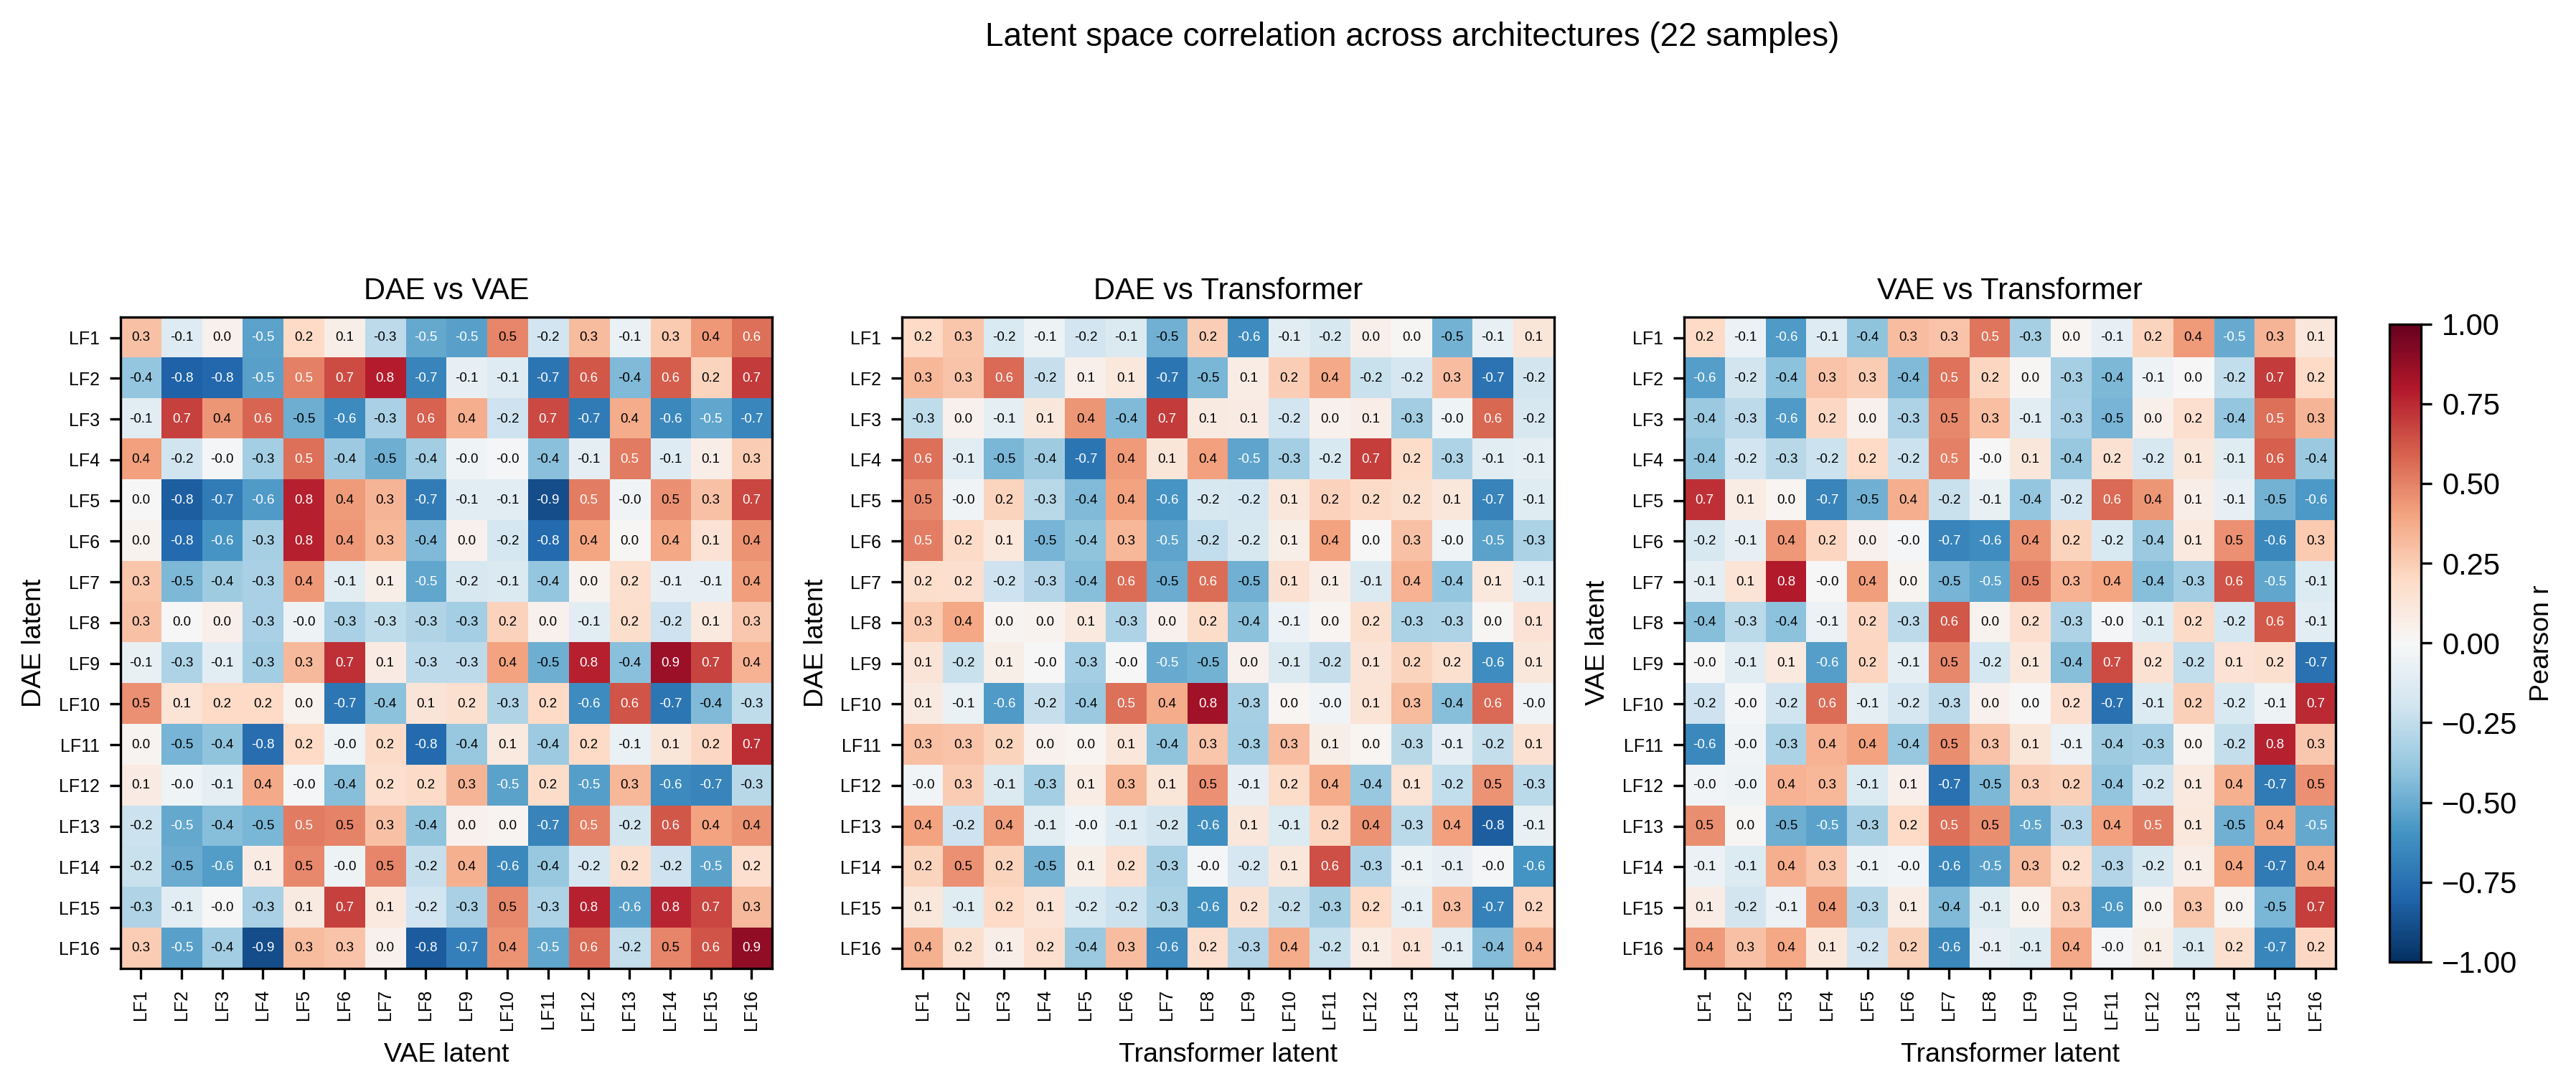
\includegraphics[width=\textwidth]{figures/dl_latent_correlation_heatmap.png}
\caption{}
\end{subfigure}
\hfill
\begin{subfigure}{0.32\textwidth}
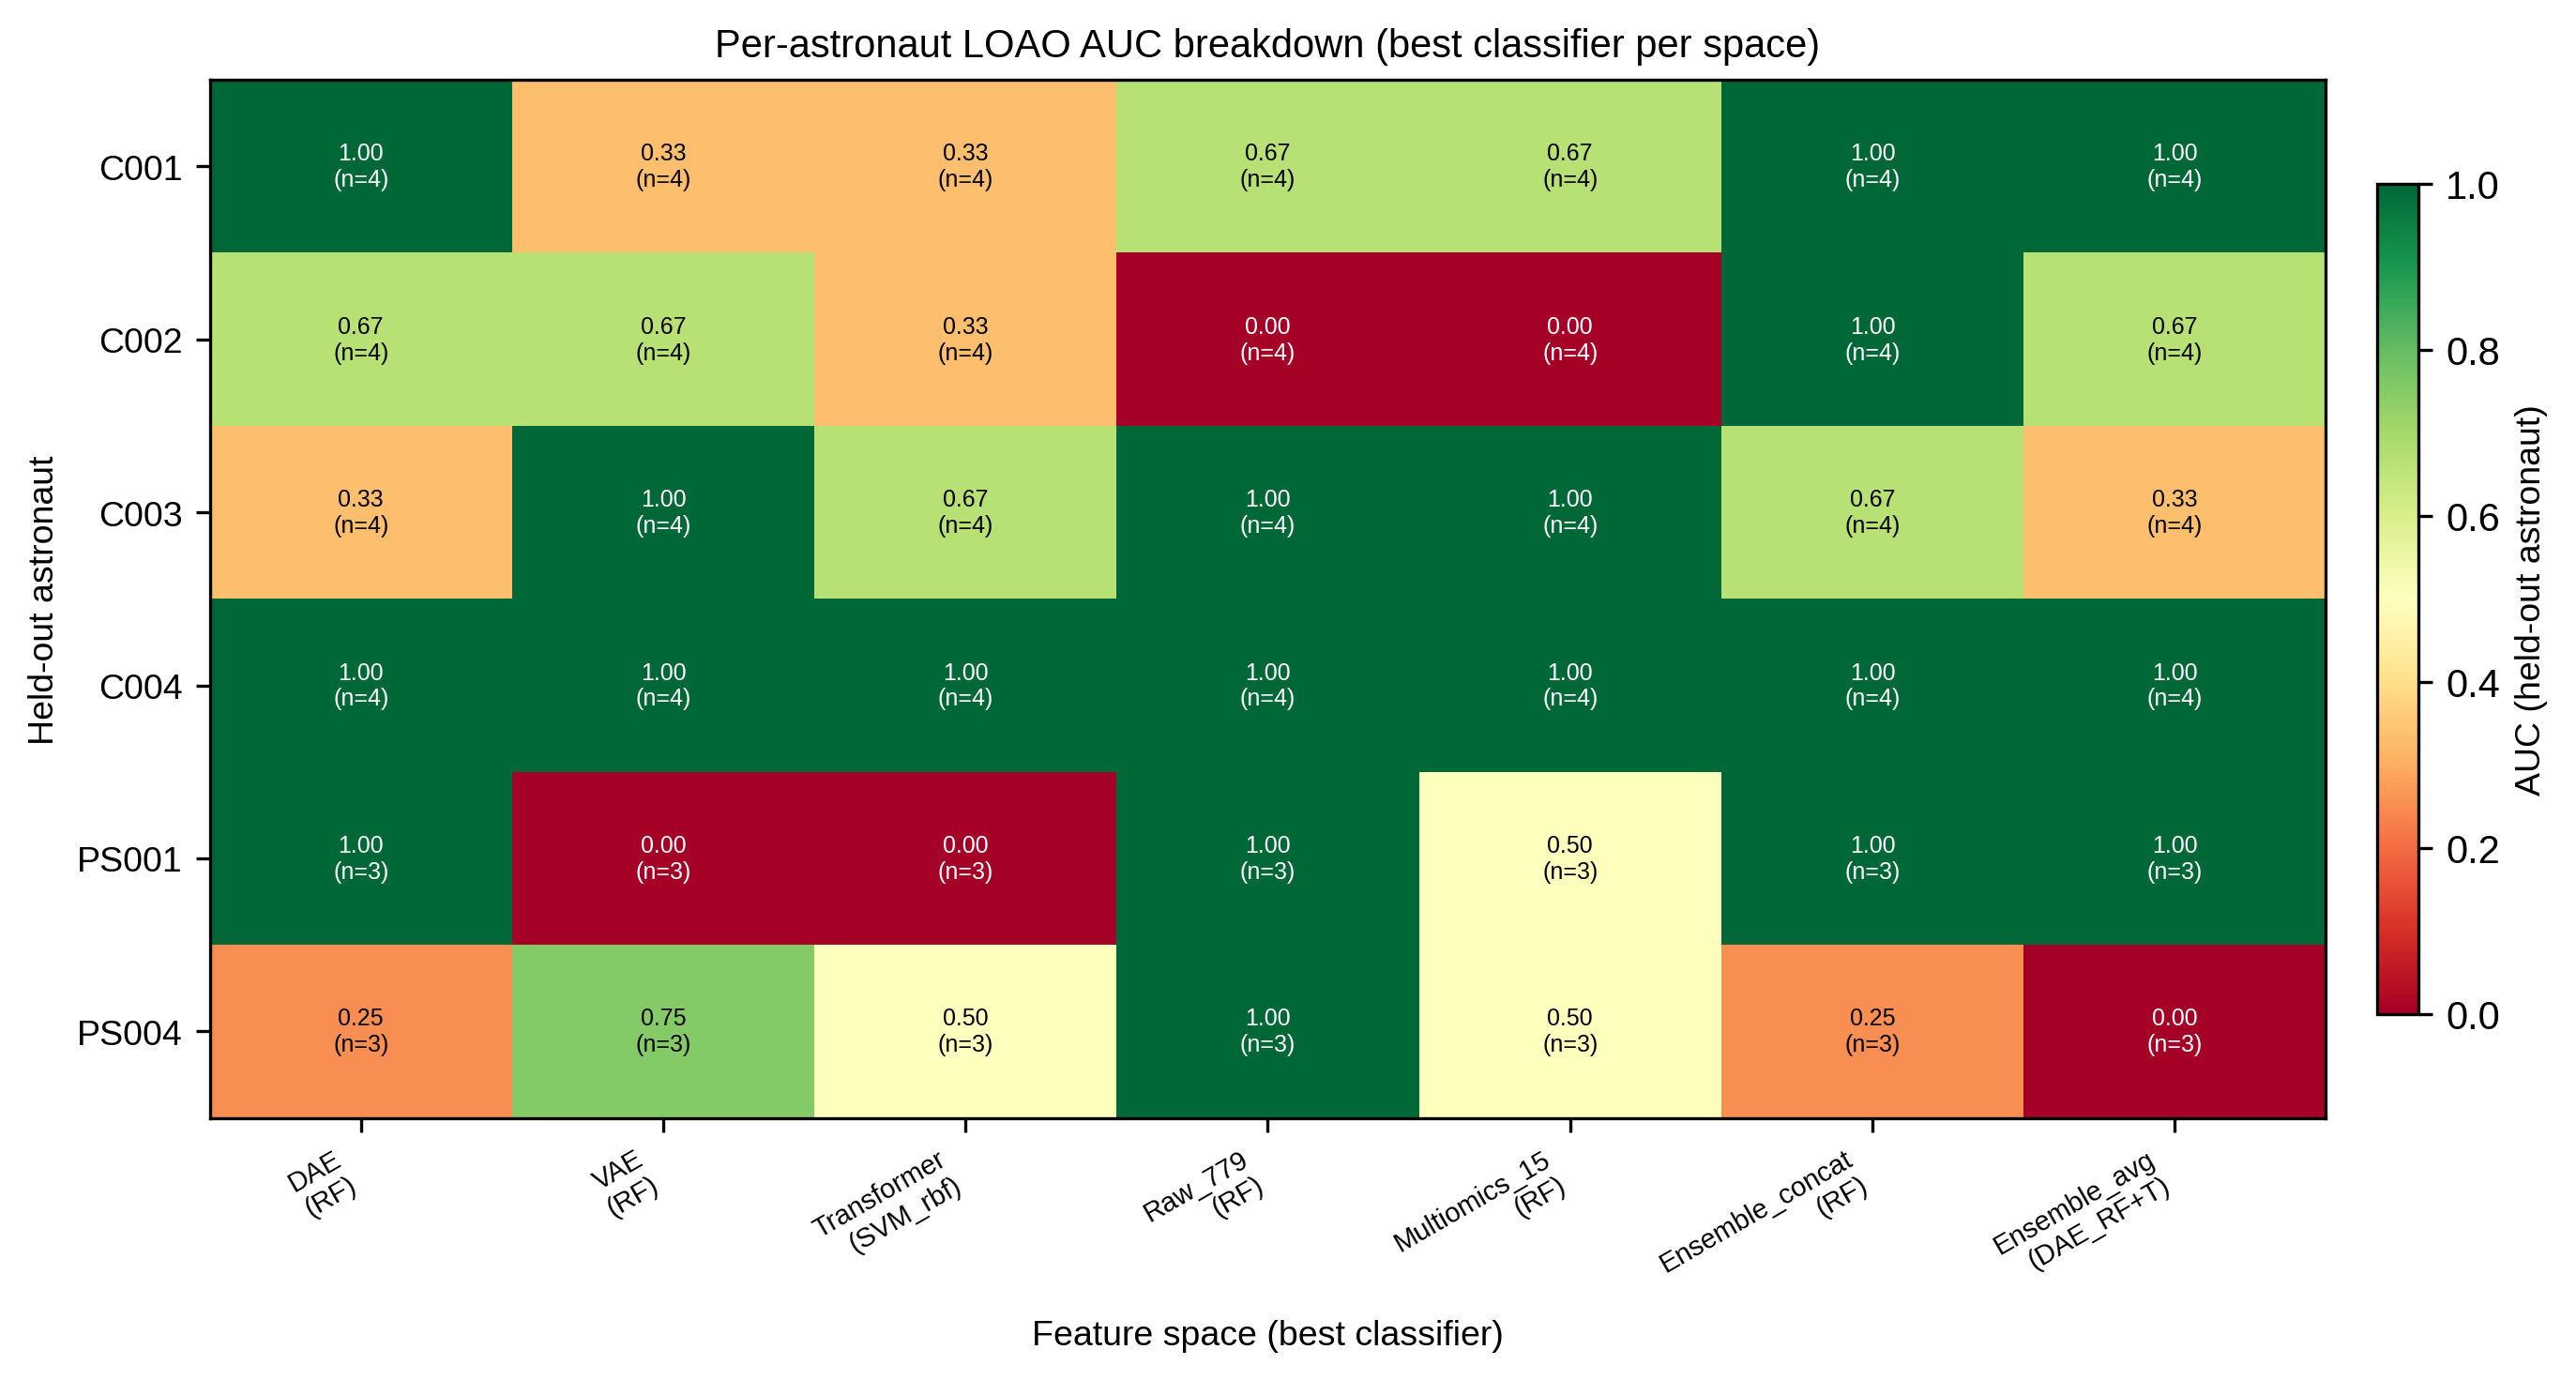
\includegraphics[width=\textwidth]{figures/dl_per_astronaut_auc.png}
\caption{}
\end{subfigure}
\caption{Architecture and ensemble comparison. (a) Pooled LOAO AUC for flight vs.\ pre-flight classification across 7 feature spaces; asterisks mark permutation $p < 0.05$. (b) ROC curves for the best classifier per architecture, including both ensemble strategies. (c) Best $|r|$ for mineral regression (I4 only, 4 targets). (d) UMAP comparison of 16-dimensional latent spaces (22 samples, 6 astronauts). (e) Pairwise Pearson correlation between latent dimensions of DAE, VAE, and FT-Transformer (16$\times$16 each); weak correlations confirm architecture-specific representations. (f) Per-astronaut LOAO AUC for the best classifier per feature space; sample counts annotated (3--4 test samples per astronaut).}
\label{fig:dl_extended}
\end{figure}

\subsection{Cross-species meta-analysis: muscle-specific concordance}

To assess whether mineral-pathway transcriptional responses are conserved across species, we conducted a Fisher $z$ random-effects meta-analysis across 28 rodent spaceflight datasets from the NASA OSDR, comprising 10 liver, 12 muscle (6 subtypes: EDL, gastrocnemius, quadriceps, soleus, tibialis anterior), and 6 kidney datasets. For each dataset, flight vs.\ ground control differential expression was computed, mapped to human orthologs, and correlated with astronaut peripheral blood mineral-pathway log$_2$FC values.

Skeletal muscle showed significant pooled concordance with astronaut mineral-pathway responses ($r = 0.035$, 95\% CI: 0.012--0.058, $p = 0.0025$; Figure~\ref{fig:cross_species}). The soleus muscle, a postural muscle particularly sensitive to microgravity unloading\textsuperscript{10}, showed the strongest tissue-specific concordance ($r = 0.059$, 95\% CI: 0.015--0.104, $p = 0.009$). Liver ($r = -0.010$, $p = 0.50$) and kidney ($r = -0.016$, $p = 0.40$) showed no significant concordance. Across all 28 datasets combined, the pooled effect was not significant ($r = 0.008$, $p = 0.41$), with moderate heterogeneity ($I^2 = 31\%$).

\begin{figure}[H]
\centering
\begin{subfigure}{0.55\textwidth}
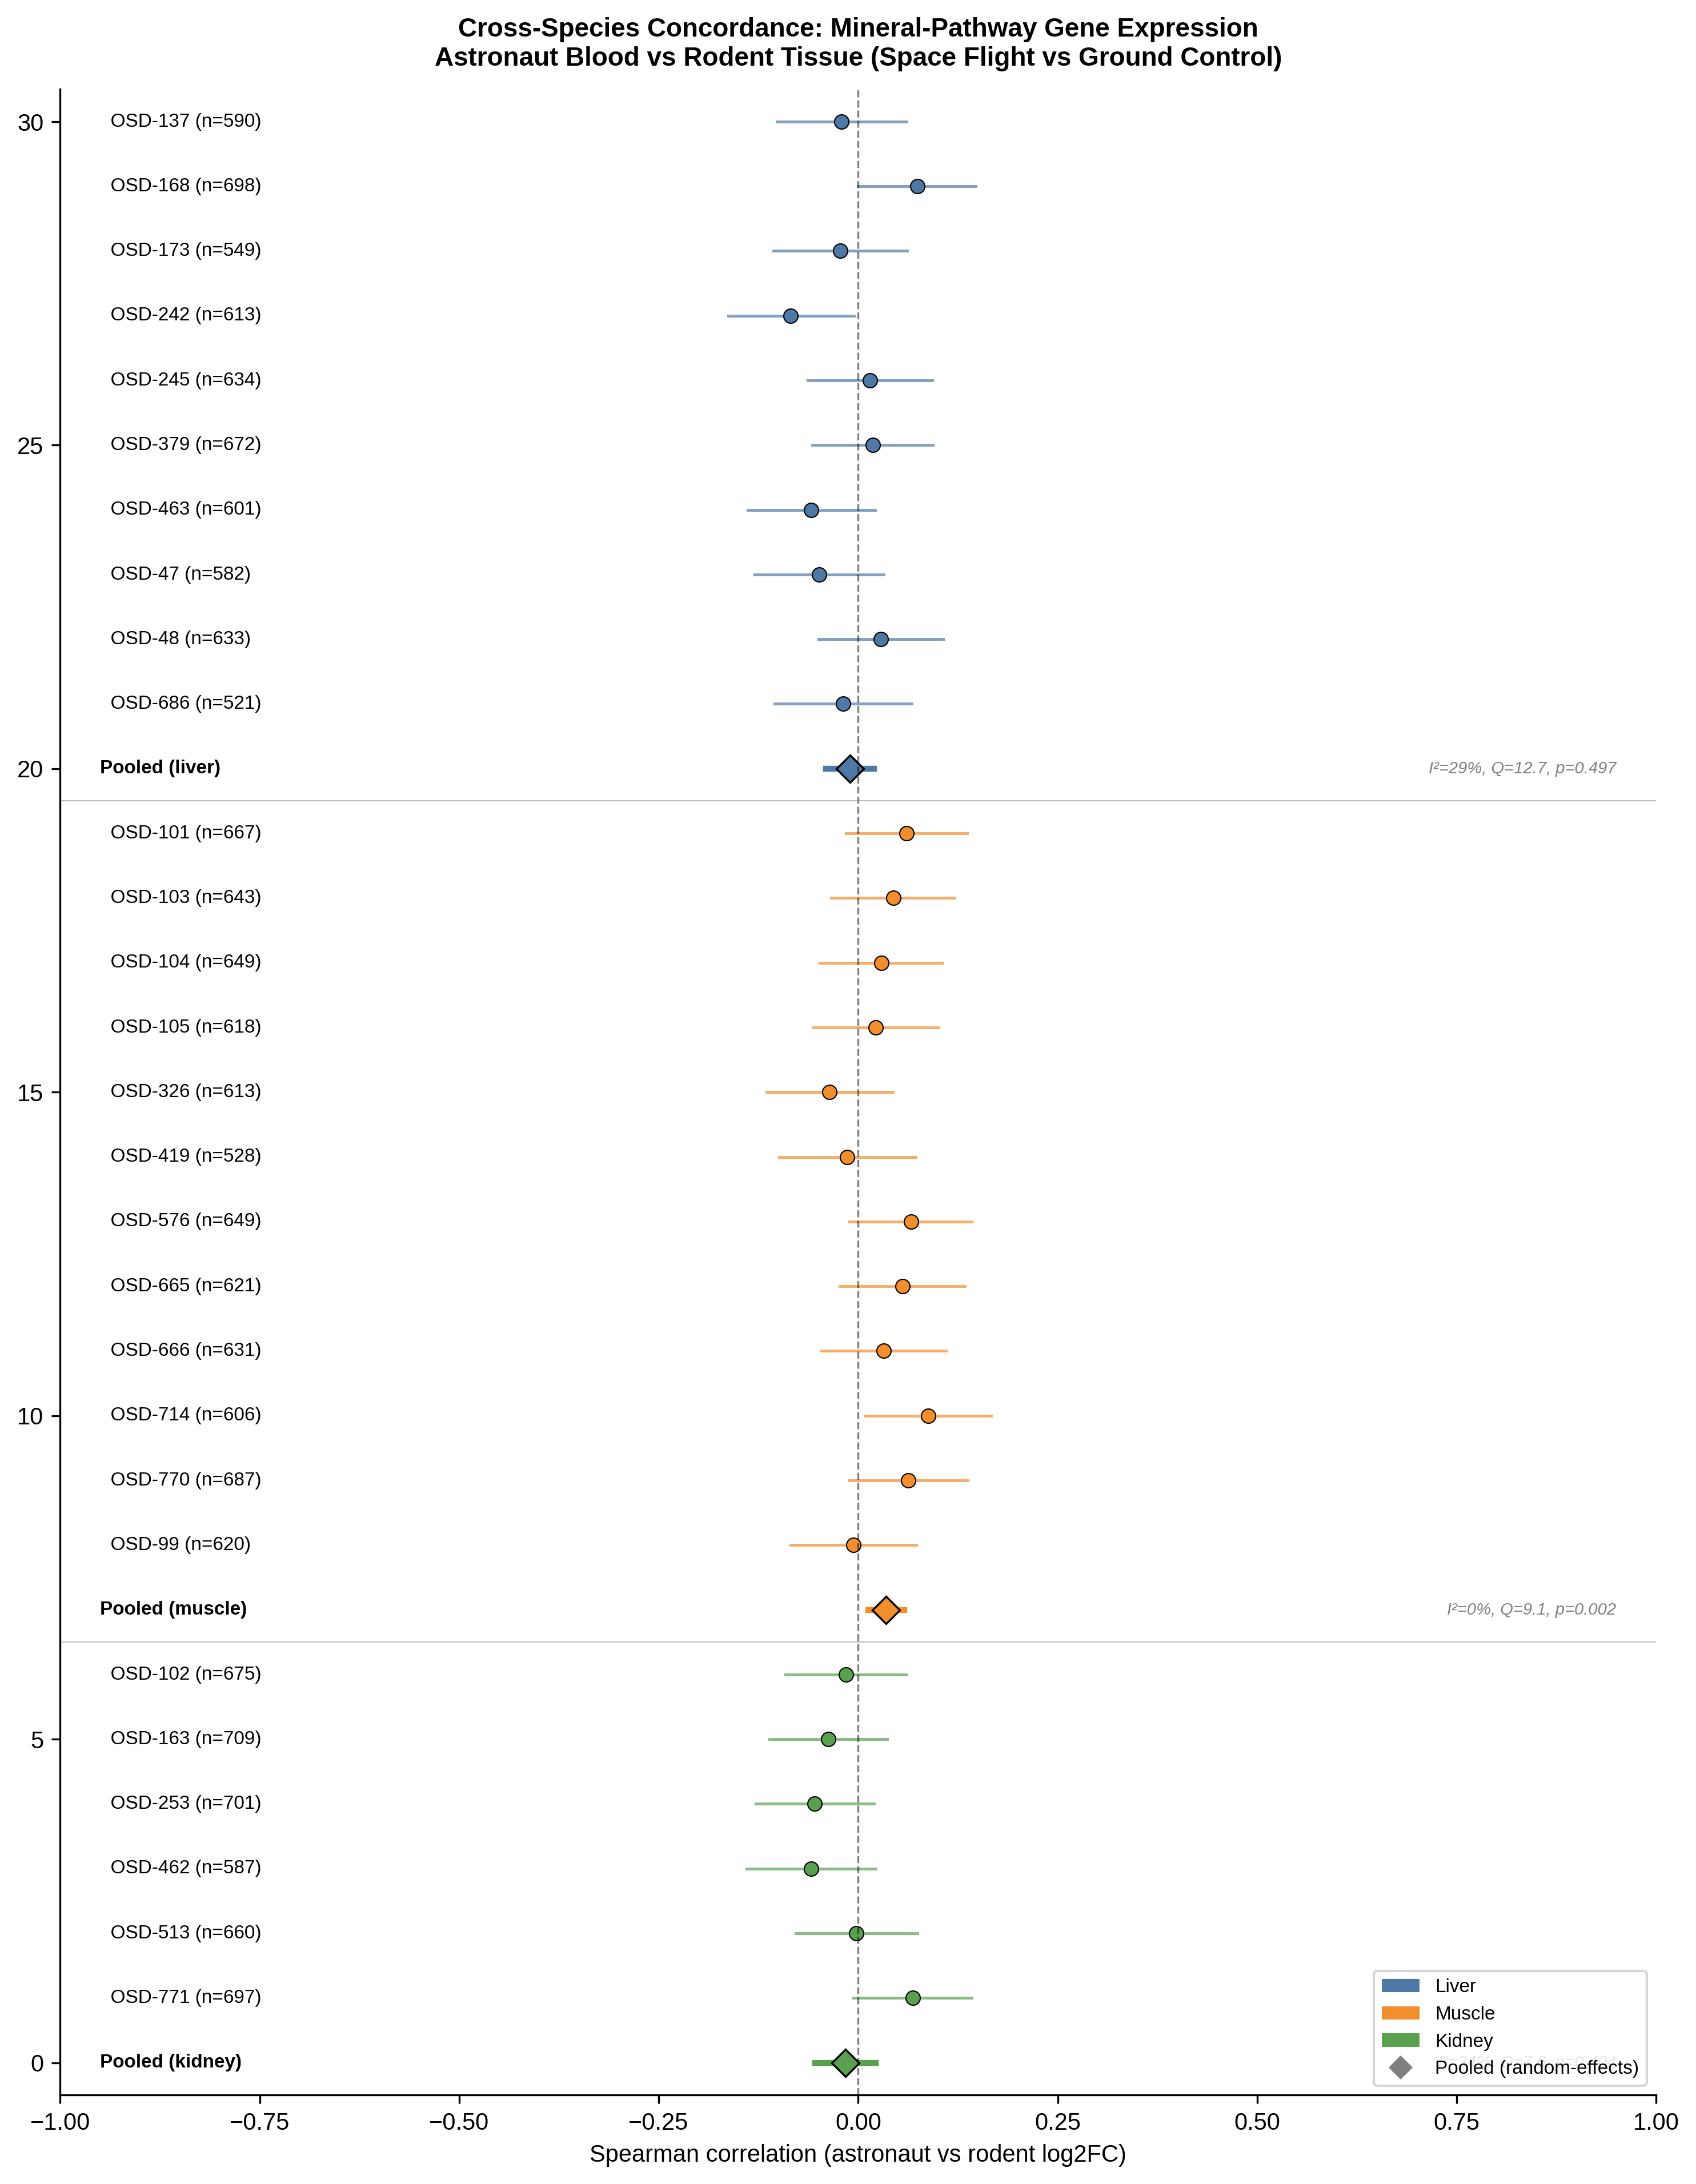
\includegraphics[width=\textwidth]{figures/figS3_forest_cross_species.png}
\caption{}
\end{subfigure}
\hfill
\begin{subfigure}{0.43\textwidth}
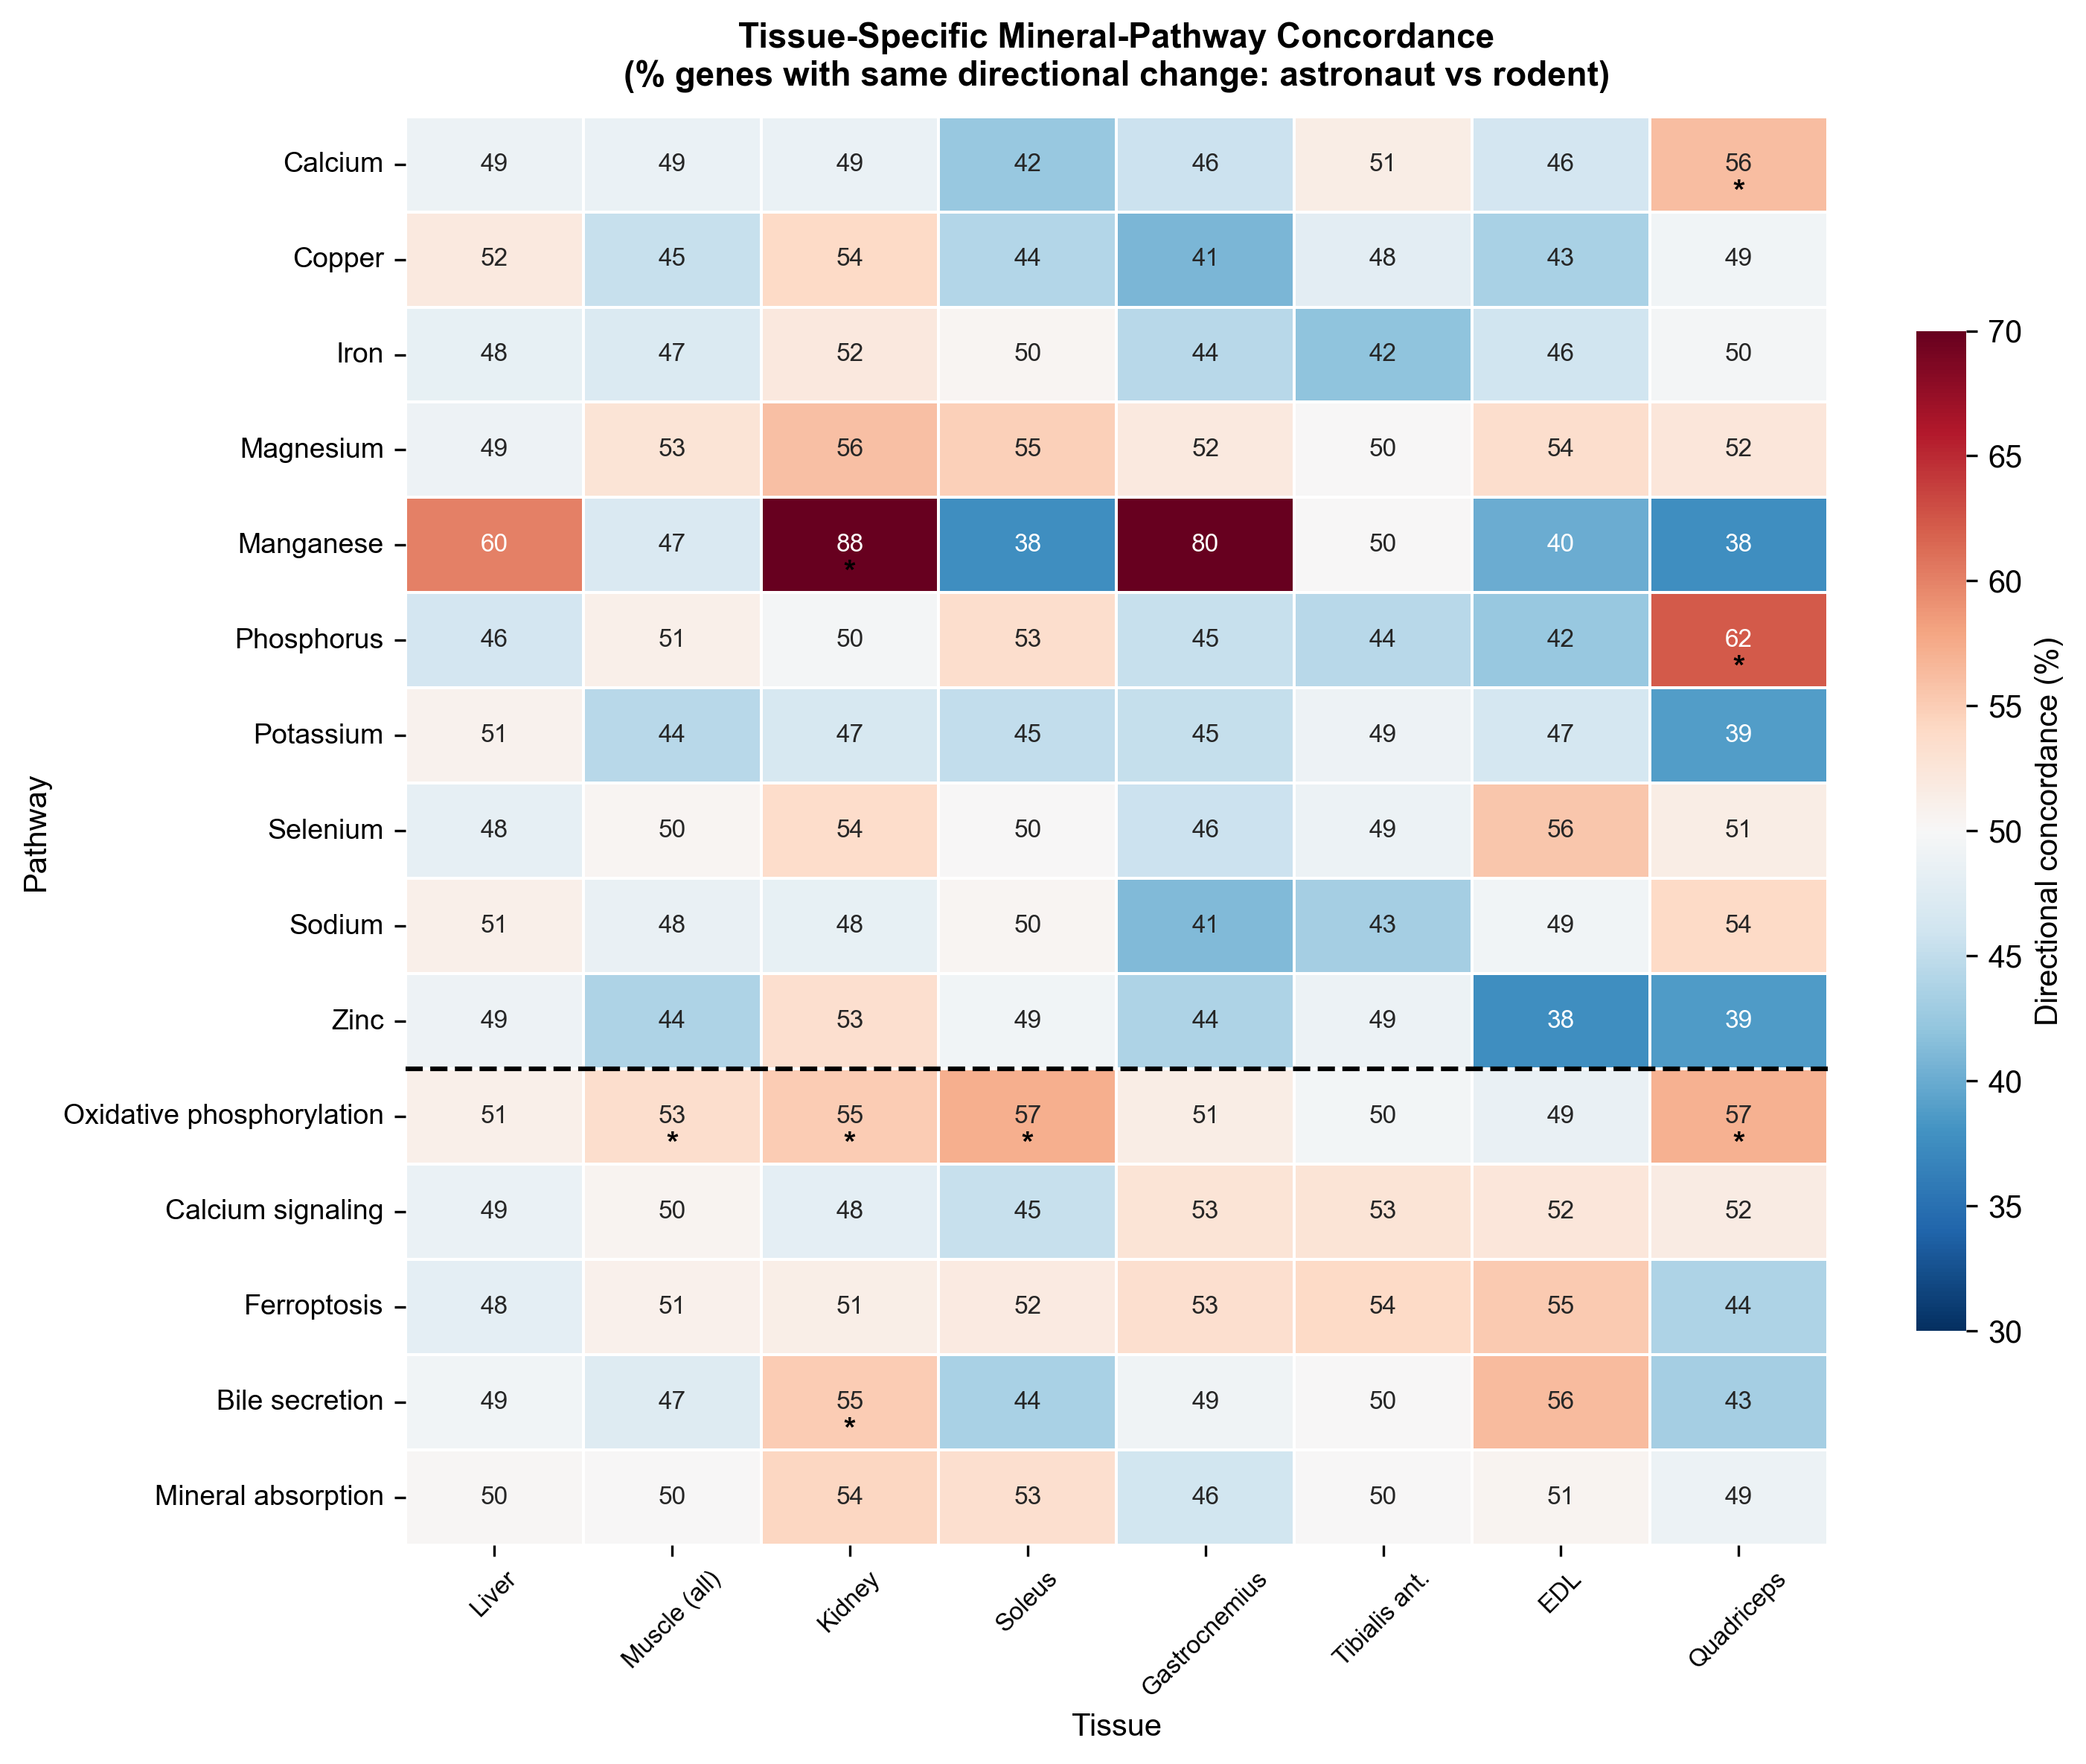
\includegraphics[width=\textwidth]{figures/figS4_tissue_pathway_heatmap.png}
\caption{}
\end{subfigure}

\vspace{0.5em}
\begin{subfigure}{0.65\textwidth}
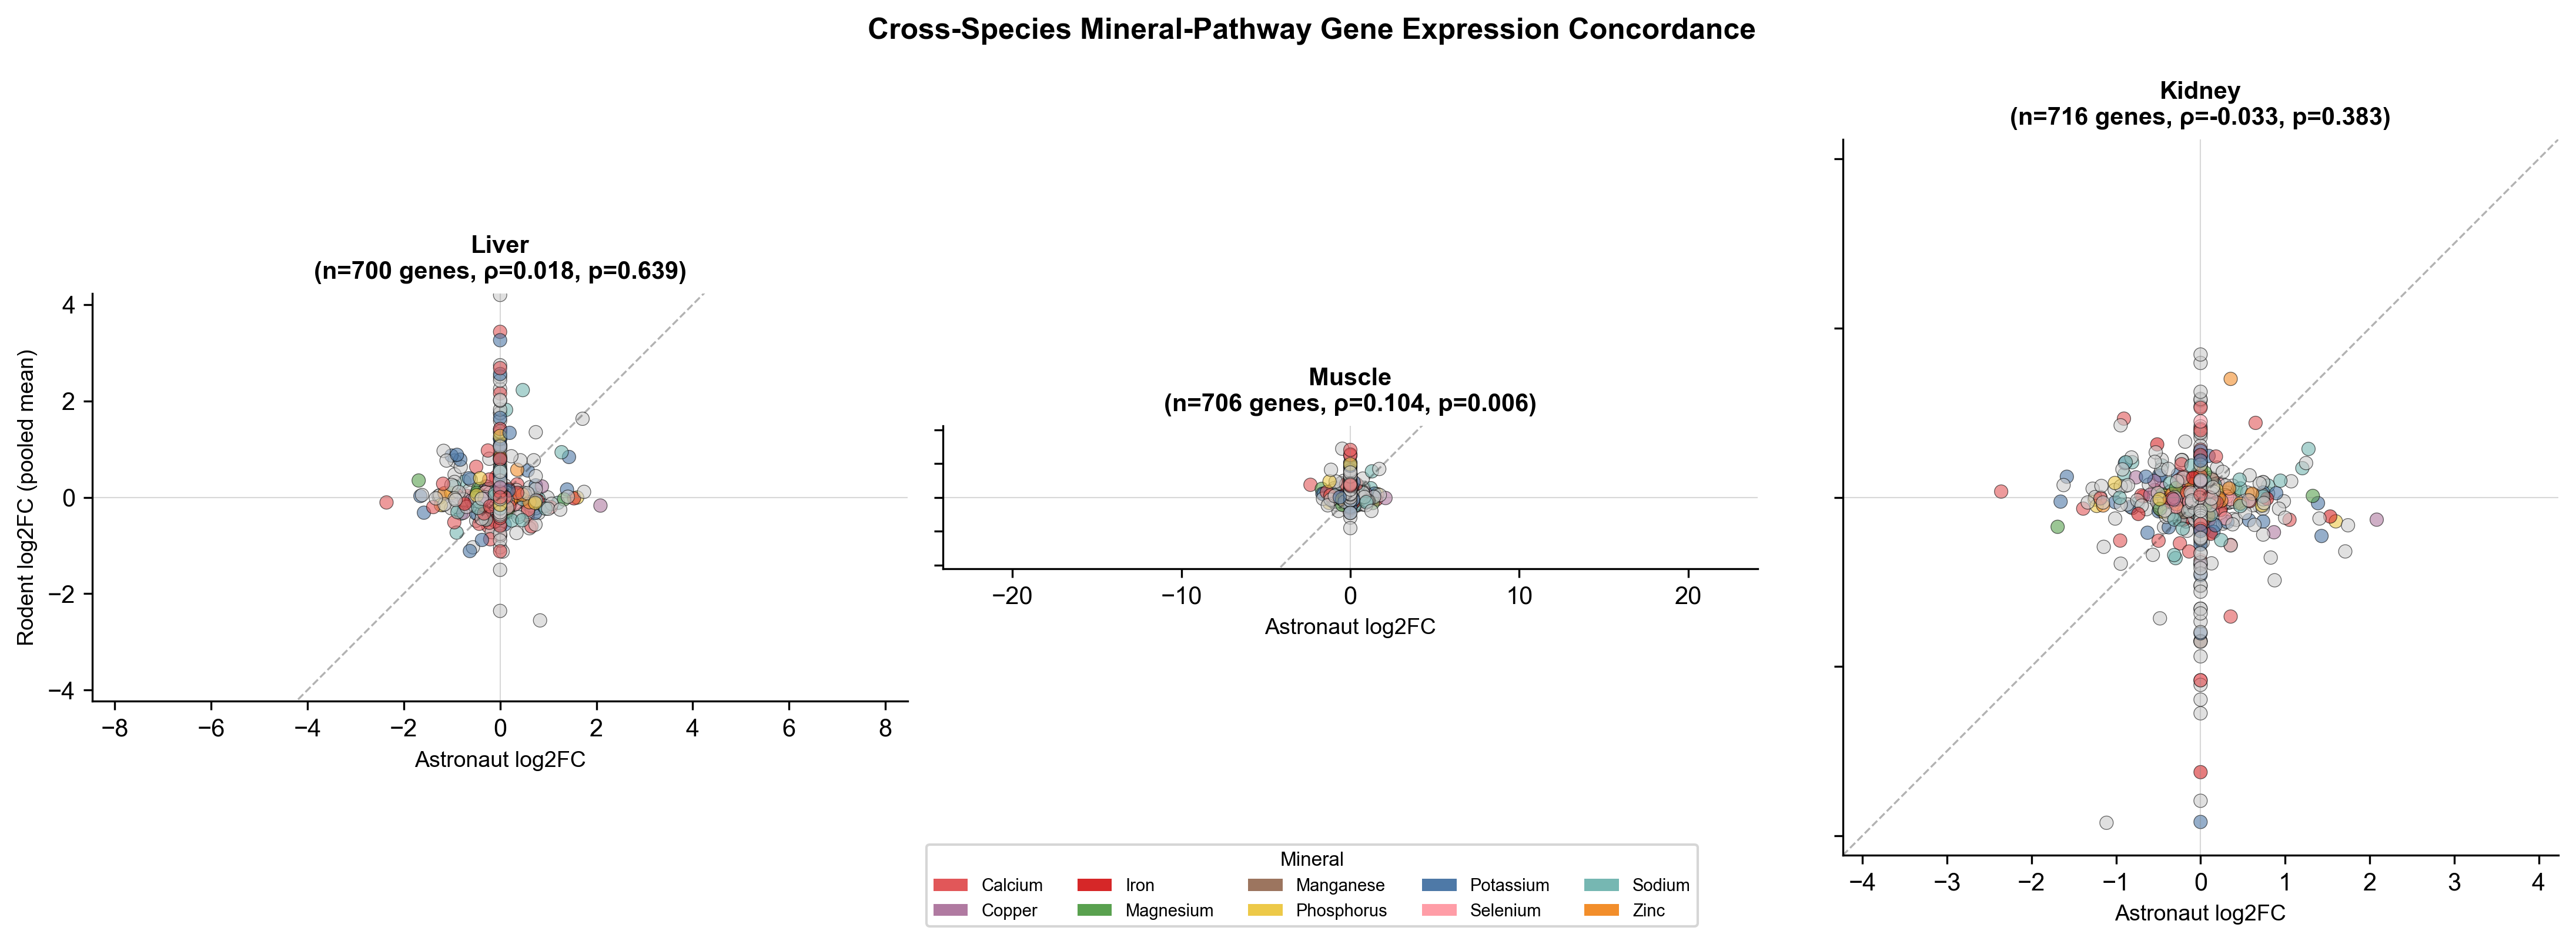
\includegraphics[width=\textwidth]{figures/figS5_scatter_cross_species.png}
\caption{}
\end{subfigure}
\caption{Cross-species meta-analysis of mineral-pathway concordance. (a) Forest plot showing Fisher $z$ random-effects pooled correlation (astronaut blood vs.\ rodent tissue) by tissue type. Diamond width represents study weight; horizontal lines show 95\% CI. (b) Tissue $\times$ pathway heatmap showing concordance proportions for each mineral pathway across tissues; asterisks mark uncorrected one-sided binomial $p < 0.05$. (c) Cross-species scatter plot of astronaut vs.\ rodent mineral-pathway log$_2$FC values, colored by tissue type, with regression line and 95\% CI.}
\label{fig:cross_species}
\end{figure}

The muscle-specific concordance pattern supports the hypothesis that skeletal muscle serves as a primary sensor and responder to mineral-pathway disruption in microgravity, consistent with the known effects of mechanical unloading on skeletal muscle\textsuperscript{10}. The absence of liver and kidney concordance likely reflects tissue-specific mineral handling and the confounding effects of comparing peripheral blood (astronaut) with internal organs (rodent). The cross-species scatter plot (Figure~\ref{fig:cross_species}c) visualizes the gene-level concordance, and the full meta-analysis summary is provided in Table~\ref{tab:meta_summary}.

\begin{table}[H]
\centering
\caption{Cross-species meta-analysis summary by tissue. Fisher $z$ random-effects pooled correlation between astronaut peripheral blood and rodent tissue mineral-pathway log$_2$FC values.}
\label{tab:meta_summary}
\begin{tabular}{lrrrrr}
\toprule
\textbf{Tissue} & \textbf{$k$} & \textbf{Pooled $r$} & \textbf{95\% CI} & \textbf{$p$-value} & \textbf{$I^2$ (\%)} \\
\midrule
Liver & 10 & $-0.010$ & $[-0.040, 0.020]$ & 0.497 & 29.3 \\
Muscle (all) & 12 & 0.035 & $[0.012, 0.058]$ & 0.002 & 0.0 \\
\quad Soleus & 3 & 0.059 & $[0.015, 0.104]$ & 0.009 & 0.0 \\
\quad EDL & 2 & 0.025 & $[-0.035, 0.085]$ & 0.415 & 14.2 \\
\quad Gastrocnemius & 2 & 0.026 & $[-0.047, 0.099]$ & 0.479 & 38.7 \\
\quad Quadriceps & 3 & 0.014 & $[-0.035, 0.062]$ & 0.573 & 13.4 \\
\quad Tibialis anterior & 2 & 0.045 & $[-0.010, 0.100]$ & 0.111 & 0.0 \\
Kidney & 6 & $-0.016$ & $[-0.054, 0.022]$ & 0.404 & 33.8 \\
All studies & 28 & 0.008 & $[-0.010, 0.025]$ & 0.405 & 30.8 \\
\bottomrule
\end{tabular}
\end{table}

\subsection{Systems biology integration}

A composite systems biology atlas (Figure~\ref{fig:atlas}) integrates KEGG pathway expression changes, mineral-gene set sizes, up/down-regulated DE gene counts per mineral, cross-species concordance, and the top 25 mineral-pathway DE genes into a multi-panel summary. The atlas reveals that copper and calcium pathways show the most consistent dysregulation across omics layers; in the calcium set this reflects down-regulation of the calcium-binding S100 proteins alongside calcium signaling genes with the largest individual fold changes. Iron metabolism genes emerge as a connecting thread: they are differentially expressed (ALAS2, HFE, GLRX5), enriched in ML stability-selected features (HFE 88\%, SLC11A2 81\%, ALAS2 69\%), and show concordant directional changes in rodent muscle. The mineral--gene--pathway network (Supplementary Figures~S6--S8) visualizes these connections.

\begin{figure}[H]
\centering
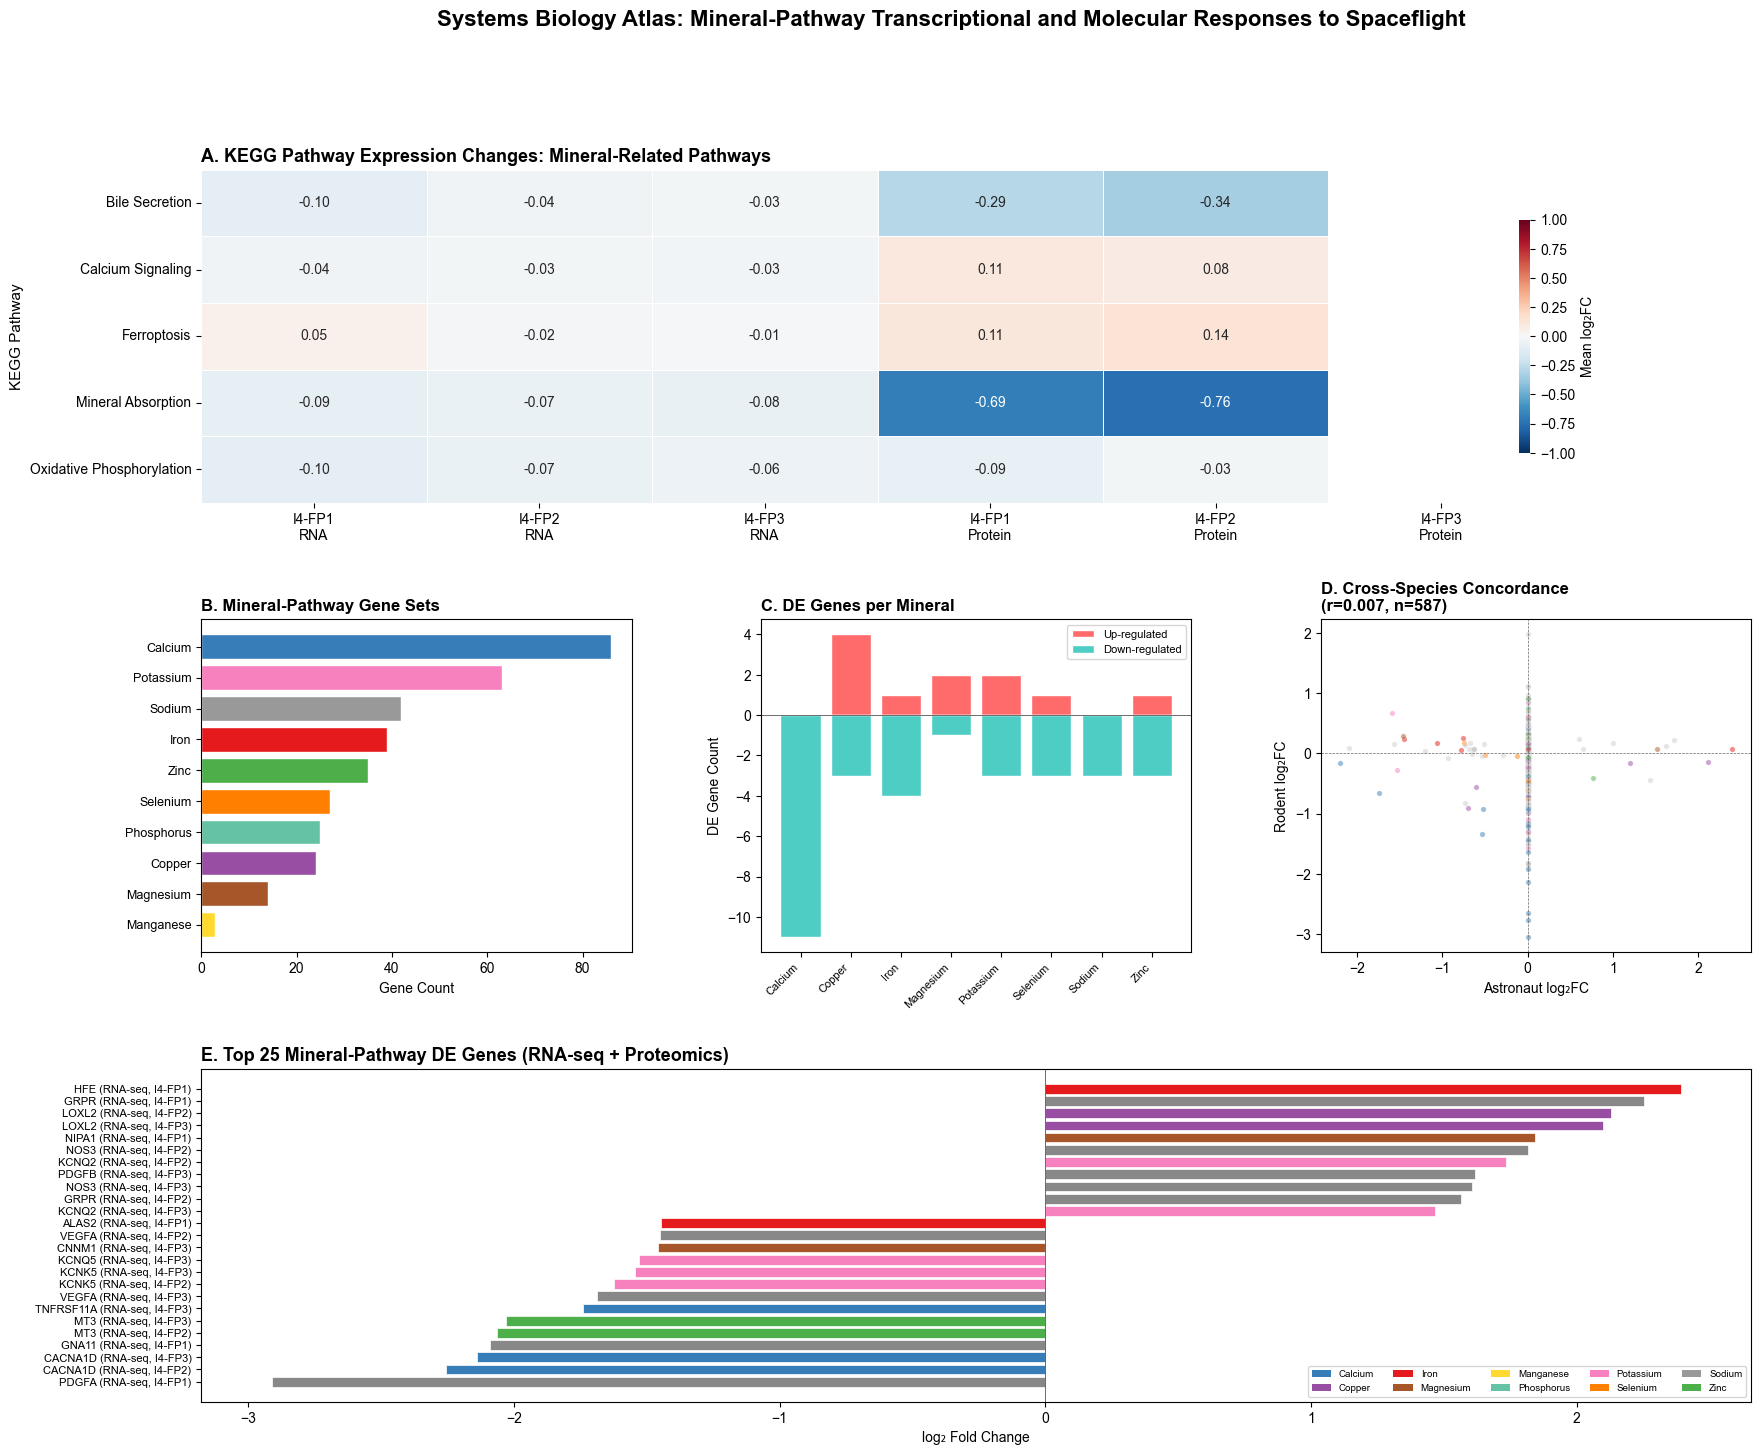
\includegraphics[width=\textwidth]{figures/fig8_systems_biology_atlas.png}
\caption{Systems biology atlas. (A) KEGG pathway mean log$_2$FC across comparisons (RNA-seq and proteomics). (B) Gene counts per mineral gene set. (C) Up/down-regulated DE genes per mineral. (D) Cross-species concordance scatter (astronaut vs.\ rodent log$_2$FC). (E) Top 25 mineral-pathway DE genes with mineral color coding.}
\label{fig:atlas}
\end{figure}

% ════════════════════════════════════════════════════════════════════
% DISCUSSION
% ════════════════════════════════════════════════════════════════════
\section{Discussion}

This study demonstrates that integrating a population reference baseline (NHANES, $n = 5{,}748$) with multi-omics astronaut data ($n = 4$) reveals mineral-pathway deviations that are invisible to within-subject analysis alone. By converting astronaut clinical measurements to population-referenced z-scores and percentile ranks, we identified markers that deviate significantly from normal population distributions --- a framing that addresses the fundamental limitation of interpreting $n = 4$ data without external context.

\subsection{Population-deviating markers: pre-existing vs.\ spaceflight-induced}

A key finding is that several population-deviating markers show deviations at pre-flight baseline. Calcium z-scores were elevated at L-92 ($d = 1.30$) and L-44 ($d = 1.92$), indicating that astronaut calcium levels sit above the 95th population percentile even before spaceflight. This pre-existing deviation may reflect the self-selection of astronauts into physically fit, nutritionally optimized individuals whose mineral status differs from the general population. MPV elevation ($d = 1.73$--$2.47$) was similarly persistent across all timepoints, suggesting a crew-level hematological characteristic rather than a spaceflight effect. These findings underscore the importance of population baselines: without NHANES, these elevated values would appear unremarkable in within-subject comparisons.

In contrast, bicarbonate depression showed a pattern consistent with both pre-existing deviation ($d = -1.24$ at L-92) and post-flight exacerbation ($d = -1.78$ at R+194), suggesting that while astronauts start below population norms, spaceflight may further suppress bicarbonate. Potassium showed a transient elevation at R+45 ($d = 1.79$) that did not survive multiple testing correction, potentially reflecting post-flight fluid rebalancing.

\subsection{Transcriptomic correlates of clinical deviations}

The population-deviating clinical markers show plausible transcriptomic correlates. The down-regulation of CACNA1D ($\log_2\text{FC} = -2.25$), the largest fold change observed, aligns with the elevated serum calcium: cellular down-regulation of calcium channels may represent an adaptive response to sustained extracellular calcium elevation. The iron pathway changes --- ALAS2 down-regulation ($\log_2\text{FC} = -1.45$) and HFE up-regulation ($\log_2\text{FC} = 2.39$) --- are consistent with suppressed erythropoiesis and altered iron sensing, aligning with the modest hemoglobin and RBC deviations from population norms. The NHANES iron status reference strengthens this interpretation: in the general population, hemoglobin is the strongest CBC correlate of serum iron ($r = 0.424$) and transferrin saturation ($r = 0.412$), establishing hemoglobin as a robust proxy for iron status. The astronaut hemoglobin deviations, though modest in effect size, therefore reflect the same iron--hemoglobin axis that dominates population-level variation, and the ALAS2 down-regulation (rate-limiting enzyme in heme biosynthesis) provides a mechanistic link between the transcriptomic and clinical findings. The NHANES reference intervals for serum iron (24.0--160.0~$\mu$g/dL), ferritin (6.4--565.6~ng/mL), and transferrin saturation (7.0--55.0\%) provide the population context against which future astronaut iron status measurements could be evaluated, should direct iron marker assays be included in upcoming missions. KCNQ2 up-regulation ($\log_2\text{FC} = 1.73$) may reflect compensatory transcriptional response to potassium shifts.

The ML stability-selected features provide an independent line of evidence: iron metabolism genes (HFE, SLC11A2, ALAS2, PCBP2) were consistently selected across LOO folds, bridging the clinical hematology findings with the transcriptomic response. The potassium channel gene KCNE1 (94\% selection frequency) connects the regression finding (potassium $r = 0.50$) with the classification analysis.

\subsection{Deep learning integration and cross-mission validation}

The denoising autoencoder analysis, integrating I4 ($n = 4$) and AX-1 ($n = 2$) astronauts, demonstrates that dimensionality reduction from 779 to 16 latent features improves flight-vs-ground classification generalization (AUC 0.728 vs.\ 0.621 for raw expression). This is consistent with the expectation that in extreme small-$n$ settings, feature compression acts as a regularizer that mitigates overfitting. The UMAP visualization (Figure~\ref{fig:dl_results}a) shows partial separation of pre- and post-flight samples, though astronaut-level clustering is also visible --- reflecting individual baseline variation that the autoencoder preserves alongside the flight signal.

The JAXA6 cross-mission validation provides the most compelling external evidence: ALAS2, the rate-limiting enzyme in erythroid heme biosynthesis, is significantly downregulated during spaceflight in both I4 (log$_2$FC $= -1.45$, $p = 10^{-5}$) and JAXA6 (logFC $= -0.80$), reaching meta-analytic significance (FDR $= 0.021$). This converges with the known spaceflight-induced anemia phenotype\textsuperscript{6} and the ML stability selection of ALAS2 (69\% selection frequency). The magnesium transporter CNNM4, identified by ML stability selection, was independently significant in JAXA6 (adj-$P = 0.045$), providing a second cross-mission validated biomarker. While the overall sign concordance (68.8\%) did not reach statistical significance ($p = 0.105$), the directional trend across 16 overlapping genes is consistent with a shared mineral-pathway transcriptional response across independent missions and agencies (NASA, JAXA).

The architecture comparison (DAE vs.\ VAE vs.\ FT-Transformer) reveals that the DAE's reconstruction objective is better suited to this extreme small-$n$ regime than the VAE's KL-regularized objective. The VAE's failure to reach classification significance (AUC = 0.621, $p = 0.143$) likely reflects over-compression: the KL penalty forces the latent distribution toward a standard normal, discarding astronaut-specific variance that is informative for flight-status discrimination when $n = 6$. The FT-Transformer, despite having 117,707 parameters (vs.\ the DAE's $\sim$200K), achieved significant classification with SVM-RBF (AUC = 0.661, $p = 0.006$), demonstrating that attention-based feature tokenization can learn useful representations even from 22 samples when heavily regularized. The fact that the transformer's optimal classifier differs from the DAE's (SVM-RBF vs.\ random forest) suggested the two architectures encode complementary information --- a hypothesis confirmed by the prediction-averaging ensemble, which achieved the highest AUC of any configuration (0.750, $p = 0.008$). Notably, the concatenation ensemble (32-dim) underperformed both the DAE alone and the averaging ensemble, indicating that feature-level fusion introduces noise in the small-$n$ regime while decision-level fusion preserves the complementary signals. The latent correlation analysis (Figure~\ref{fig:dl_extended}e) further supports this: weak inter-architecture correlations ($|r| < 0.5$ for most dimension pairs) confirm that each architecture discovers different projections of the 779-gene space. The 15-gene multi-omics consensus set (AUC = 0.598) did not improve over raw expression, indicating that proteomics-informed gene filtering does not substitute for learned dimensionality reduction in this context.

\subsection{Cross-species concordance: muscle as mineral sensor}

The 28-dataset meta-analysis revealed that skeletal muscle --- particularly the soleus --- shows significant concordance with astronaut mineral-pathway responses, while liver and kidney do not. This tissue-specific pattern is biologically plausible: the soleus is a postural muscle that undergoes profound atrophy in microgravity\textsuperscript{10}, and muscle tissue is a major reservoir of intracellular minerals (particularly magnesium and potassium). The concordance effect sizes are small ($r = 0.035$--$0.059$), which is expected given the differences in species (human vs.\ mouse), tissue (blood vs.\ muscle), mission duration (3 days vs.\ 21--90 days), and spaceflight environment (LEO vs.\ ISS). Nevertheless, the statistical significance ($p = 0.002$--$0.009$) across 12 independent muscle datasets provides robust evidence for a conserved mineral-pathway response in skeletal muscle.

\subsection{Limitations}

Several limitations must be acknowledged. First, the astronaut sample size ($n = 4$) is severely underpowered; one-sample tests at each timepoint have minimal statistical power, and we emphasize effect sizes over $p$-values. Second, exact age and sex of individual crew members were not available in the provided dataset; the all-sexes age 40--60 reference was used as the primary baseline. Third, NHANES uses a complex survey design; we used unweighted statistics for reference interval derivation, which is standard practice but may slightly bias population estimates. Fourth, the cross-species comparison is confounded by tissue, mission duration, and species differences. Fifth, the SVM classification AUC $= 1.0$ result must be interpreted with caution due to the non-standard permutation null distribution caused by class weighting. Sixth, the regression $R^2$ values are low (0.12--0.19), indicating that mineral-pathway gene expression explains only a modest fraction of serum mineral variance. Seventh, this is an observational study; no causal inference about spaceflight effects on mineral homeostasis can be drawn. Eighth, the deep learning analysis integrates only 6 astronauts (I4 + AX-1); while the autoencoder improves classification generalization, the regression results show negative correlations (a LOAO artifact with $n = 4$), and reliable individual-level mineral prediction requires larger cohorts. Ninth, JAXA6 provides group-mean expression rather than per-sample data, limiting validation to signature concordance rather than independent classification. Tenth, the architecture comparison (DAE vs.\ VAE vs.\ FT-Transformer) is limited to 500 (classification) and 100 (regression) permutations due to computational cost, and the Raw\_779 regression p-values were not computed (779-dimensional permutation tests are prohibitively slow on CPU); the regression $|r|$ values for raw expression are reported without significance testing.

% ════════════════════════════════════════════════════════════════════
% METHODS
% ════════════════════════════════════════════════════════════════════
\section{Methods}

\subsection{NHANES data acquisition and reference construction}

Three consecutive NHANES cycles (2013--2014, 2015--2016, 2017--2018) were downloaded from the CDC website (\texttt{https://wwwn.cdc.gov/Nchs/Nhanes/}). For each cycle, the Standard Biochemistry Profile (BIOPRO), Complete Blood Count with 5-part differential (CBC), and Demographics (DEMO) XPT files were retrieved and parsed using \texttt{pandas.read\_sas(format='xport')}. Files were merged on the participant identifier (SEQN). The reference population was restricted to adults aged 40--60 years (all sexes), yielding 5,748 participants. Reference statistics (mean, SD, median, percentiles P1--P99) were computed per variable for all sexes combined and stratified by sex. The 95\% reference interval was defined as P2.5--P97.5.

\subsection{NHANES iron status data}

Four iron status markers not present in the astronaut clinical panel were added as population reference context. Serum iron (LBXSIR, $\mu$g/dL) was extracted from the BIOPRO files across all three cycles ($n = 5{,}435$). Ferritin (LBXFER, ng/mL) was obtained from the NHANES Ferritin files (FERTIN\_I for 2015--2016, FERTIN\_J for 2017--2018; $n = 2{,}190$); ferritin data were not available for the 2013--2014 cycle. Transferrin saturation (LBDPCT, \%) and total iron-binding capacity (LBDTIB, $\mu$g/dL) were obtained from the TIBC and Transferrin Saturation file (FETIB\_J, 2017--2018 only; $n = 1{,}678$); TIBC files were not available for the 2013--2014 or 2015--2016 cycles. Reference statistics were computed using the same age 40--60, all-sexes restriction. Pearson correlations between each iron marker and six CBC parameters (hemoglobin, hematocrit, RBC count, MCH, MCHC, MCV) were computed on merged NHANES samples within the same age restriction.

\subsection{Astronaut data acquisition}

Astronaut data were retrieved from the NASA OSDR REST API (\texttt{https://visualization.osdr.nasa.gov/biodata/api}). Studies included: OSD-569 (RNA-seq), OSD-571 (proteomics and metabolomics DE), OSD-575 (Comprehensive Metabolic Panel and CBC), and OSD-656 (urine immune panel). All data correspond to the Inspiration4 mission with four civilian astronauts (C001--C004) sampled at seven timepoints: L-92, L-44, L-3 (pre-flight), R+1 (return/flight), R+45, R+82, R+194 (post-flight). Clinical chemistry variables (calcium, potassium, sodium, chloride, bicarbonate) were from the CMP panel; hematological variables (hemoglobin, hematocrit, RBC, MCH, MCHC, MCV, WBC, RDW, platelets, MPV) were from the CBC panel.

\subsection{Population-referenced analysis}

Each astronaut measurement was converted to a z-score: $z = (x_{\text{astro}} - \mu_{\text{NHANES}}) / \sigma_{\text{NHANES}}$, where $\mu$ and $\sigma$ are the NHANES age 40--60 all-sexes mean and SD. Empirical percentile ranks were computed using the NHANES reference distribution. Measurements falling outside P2.5--P97.5 were flagged as outside the reference interval. One-sample $t$-tests (astronaut values vs.\ NHANES mean) and Wilcoxon signed-rank tests were performed at each timepoint. Cohen's $d$ was computed as $(\bar{x}_{\text{astro}} - \mu_{\text{NHANES}}) / \sigma_{\text{NHANES}}$. Benjamini--Hochberg FDR correction was applied across all 105 tests (15 variables $\times$ 7 timepoints). Three implausible values (C003 at L-92: MPV = 330 fL, RDW = 32.4\%, platelets = 12.9 $\times$ 10$^3$/uL) were identified as data entry errors and excluded.

\subsection{Mineral-pathway gene set construction}

Curated mineral homeostasis gene sets for 10 minerals (calcium, iron, magnesium, zinc, copper, selenium, potassium, sodium, phosphorus, manganese) were compiled from KEGG pathway hsa04978 (Mineral absorption), UniProt, HGNC, and published literature. Five KEGG pathways were included: hsa04978 (61 genes), hsa04020 (254 genes), hsa04216 (42 genes), hsa00190 (138 genes), and hsa04976 (90 genes). The final gene set comprised 801 unique genes, with 784 mapped to the astronaut RNA-seq feature space after ENSEMBL-to-HGNC symbol mapping via the mygene.info API (73.6\% mapping rate).

\subsection{RNA-seq differential expression}

The I4 RNA-seq data included two DE methods: DESeq2 and a pipeline-transcriptome-de approach. The pipeline-transcriptome-de method yielded meaningful fold changes (range $-2.91$ to $2.39$) and was used as the primary DE method, as DESeq2 log$_2$FC values were uniformly near zero. Three flight comparisons were analyzed: I4-FP1 (R+1 vs.\ pre-flight), I4-FP2 (R+1/R+45/R+82 vs.\ pre-flight), and I4-FP3 (all post-flight vs.\ pre-flight). Significant genes were defined as $|\log_2\text{FC}| > 0.5$ and $p < 0.05$.

\subsection{Proteomics and metabolomics}

Proteomics DE was performed using limma (I4-FP1 and I4-FP2 comparisons) with 3,285 proteins. Metabolomics DE included 2,624 metabolites across two comparisons. Proteomics data contained gene symbols; metabolomics data used metabolite identifiers.

\subsection{Gene set enrichment analysis}

GSEA was performed with \texttt{gseapy} (Python; preranked mode, 1,000 permutations, seed 42). RNA-seq genes were ranked by $\mathrm{sign}(\log_2\text{FC}) \times -\log_{10}(p)$ for each flight comparison, and proteins by the limma $t$-statistic for I4-FP1 and I4-FP2. Gene sets with fewer than 15 genes in a ranking (magnesium, manganese and phosphorus for RNA-seq) fall below gseapy's default minimum size and are not tested. Gene sets included the 10 mineral-specific gene sets and 5 KEGG pathway gene sets. Normalized enrichment scores (NES), NOM $p$-values, and FDR $q$-values were reported.

\subsection{Machine learning: regression}

Feature matrices were constructed from RNA-seq count data restricted to 784 mineral-pathway genes, log$_2$(counts + 1) transformed, with the top 200 genes by variance selected. Four regressors (Ridge, SVR-Linear, SVR-RBF, RandomForest) predicted serum calcium, potassium, sodium, and hemoglobin under LOO-CV ($n = 16$). Performance was assessed by Pearson $r$ and $R^2$. Permutation importance (20 repeats) identified key predictive genes.

\subsection{Machine learning: classification}

Class-weighted elastic-net logistic regression (\texttt{LogisticRegression(penalty='elasticnet', class\_weight='balanced', solver='saga')}) was applied with nested LOO-CV. The outer loop held out 1 of 16 samples (4 flight, 12 ground); the inner loop (3-fold stratified) selected hyperparameters (C $\in$ \{0.01, 0.05, 0.1, 0.5, 1.0\}, l1\_ratio $\in$ \{0.1, 0.3, 0.5, 0.7, 0.9\}). StandardScaler was fit inside each fold. SVM-RBF with class weights was included as a non-linear baseline. A 500-permutation test shuffled labels and reran the full LOO-CV to generate the null distribution. Stability selection tracked gene selection frequency across LOO folds.

\subsection{Cross-mission integration and deep learning}

Per-sample RNA-seq from the Axiom-1 (AX-1) mission (GEO: GSE276490; 2 astronauts, 3 timepoints: pre-flight, post-24h, post-3months) was downloaded as TPM values. I4 counts were CPM-normalized and log$_2$-transformed; AX-1 TPM values were log$_2$-transformed. Both datasets were mapped to HGNC gene symbols and intersected to 779 common mineral-pathway genes. Batch effects between studies were addressed by z-scoring each gene within each study (removing study-specific mean and variance while preserving within-study biological variation).

A denoising autoencoder was implemented in PyTorch with architecture 779 $\to$ 128 $\to$ 64 $\to$ 16 (latent) $\to$ 64 $\to$ 128 $\to$ 779, using BatchNorm, ReLU activations, dropout (0.3), and $L_2$ weight decay ($10^{-4}$). Gaussian noise ($\sigma = 0.1$) was added to inputs during training. The model was trained for up to 300 epochs with early stopping (patience = 30) using Adam optimizer (lr = $10^{-3}$). Leave-one-astronaut-out (LOAO) cross-validation was performed across 6 astronauts (4 I4 + 2 AX-1), with latent features extracted from held-out samples to prevent information leakage.

Classification (flight vs.\ pre-flight) was performed on the 16-dimensional latent space using logistic regression, SVM (RBF and linear kernels), and random forest, with LOAO CV and a 1000-permutation test (shuffling training labels within each fold). Regression (calcium, potassium, sodium, hemoglobin) was performed on I4 samples only ($n = 16$) using Ridge, SVR, and random forest regressors with LOAO CV and 1000-permutation tests.

\subsubsection{Alternative architectures}

A $\beta$-VAE ($\beta = 0.5$) with the same encoder/decoder dimensions was trained with the reparameterization trick and loss $= \text{MSE} + \beta \cdot \text{KL}$. A lightweight FT-Transformer treated each of the 779 genes as a token with a value embedding (16-dim) and a learned gene-identity embedding. A single transformer encoder layer (4 attention heads, FFN dimension 32, pre-LN, GELU activation, dropout 0.5) processed the token sequence, and a CLS token produced the 16-dimensional latent. The decoder (16 $\to$ 128 $\to$ 779) enabled reconstruction loss training. Both models used LOAO CV identical to the DAE. Classification and regression evaluation used 500 and 100 permutations, respectively (reduced from 1000 due to computational cost). For the multi-omics consensus baseline, 15 genes overlapping between RNA-seq mineral-pathway genes and proteomics DE genes ($p < 0.05$) were used directly as features without encoding.

\subsubsection{Ensemble strategies}

Two ensemble approaches were evaluated. (1) \textit{Concatenation}: DAE and FT-Transformer 16-dimensional latent features were concatenated into a 32-dimensional feature matrix and evaluated with the same 4 classifiers under LOAO CV with 500 permutations. (2) \textit{Prediction averaging}: per-sample predicted probabilities from the best DAE classifier (DAE+RF) and the best FT-Transformer classifier (Transformer+SVM-RBF) were averaged arithmetically; the permutation test retrained both classifiers within each LOAO fold with shuffled labels and averaged their predictions. Latent space correlations were computed as pairwise Pearson correlations between all 16 latent dimensions across architectures (16$\times$16 matrices). Per-astronaut AUC was computed from the LOAO held-out predictions for each astronaut individually (3--4 test samples per astronaut).

\subsubsection{JAXA6 validation}

JAXA6 plasma cell-free RNA-seq differential expression (OSD-530; 6 Japanese astronauts, group-mean expression for 11 time points) was obtained from the associated data repository. As JAXA6 provides group means rather than per-sample data, it was used exclusively for signature validation. Concordance between I4 (I4-FP1) and JAXA6 flight-vs-pre log$_2$FC values was assessed by sign concordance (binomial test), Pearson correlation, and Fisher's exact test for enrichment of I4 DE genes in JAXA6 DE genes (adj-$P < 0.05$). A weighted Stouffer meta-analysis combined I4 and JAXA6 $p$-values (weighted by $\sqrt{n}$ per mission), with Benjamini--Hochberg FDR correction. ML stability-selected genes were checked for presence in the JAXA6 DE table.

\subsection{Cross-species meta-analysis}

Twenty-eight rodent spaceflight datasets were retrieved from the NASA OSDR, comprising 10 liver, 12 muscle (EDL, gastrocnemius, quadriceps, soleus, tibialis anterior), and 6 kidney datasets. For each dataset, flight vs.\ ground control DE was computed using Welch's $t$-tests with Benjamini--Hochberg correction. Mouse ENSEMBL IDs were mapped to human gene symbols via mygene.info homologene data. Fisher $z$ random-effects meta-analysis was performed by tissue type, pooling individual study $z$-transformed correlations between astronaut and rodent mineral-pathway log$_2$FC values. Heterogeneity was assessed using Cochran's $Q$ and $I^2$.

\subsection{Statistical methods}

All statistical analyses were performed in Python 3.11 using \texttt{scipy}, \texttt{statsmodels}, \texttt{scikit-learn}, and \texttt{pandas}. Multiple testing correction used Benjamini--Hochberg FDR. Effect sizes were reported as Cohen's $d$ for group comparisons and Pearson $r$ for correlations. Reference intervals were defined as P2.5--P97.5 (95\% interval) and P5--P95 (90\% interval).

\subsection{Reproducibility}

All analysis scripts, processed data, figures, and a data dictionary are available in a FAIR-compliant Zenodo package. Scripts are numbered 01--11, covering data acquisition, processing, ML analysis, visualizations, cross-species meta-analysis, NHANES integration, and supplementary outputs. Python 3.11 with \texttt{scipy}, \texttt{scikit-learn}, \texttt{pandas}, \texttt{matplotlib}, and \texttt{statsmodels} was used throughout.

% ════════════════════════════════════════════════════════════════════
% REFERENCES
% ════════════════════════════════════════════════════════════════════
\section*{References}

\begin{thebibliography}{99}

\bibitem{williams2009}
Williams D, Kuipers A, Mukai C, Thirsk R. Acclimation during space flight: effects on human physiology. \textit{CMAJ}. 2009;180(13):1317--1323. doi:10.1503/cmaj.090628

\bibitem{norsk2015}
Norsk P, Asmar A, Damgaard M, Christensen NJ. Fluid shifts, vasodilatation and ambulatory blood pressure reduction during long duration spaceflight. \textit{J Physiol}. 2015;593(3):573--584. doi:10.1113/jphysiol.2014.284869

\bibitem{stein2002}
Stein TP. Space flight and oxidative stress. \textit{Nutrition}. 2002;18(10):867--871. doi:10.1016/S0899-9007(02)00938-3

\bibitem{overbey2024}
Overbey EG, Kim J, Tierney BT, et al. The Space Omics and Medical Atlas (SOMA) and international astronaut biobank. \textit{Nature}. 2024;632(8027):1145--1154. doi:10.1038/s41586-024-07639-y

\bibitem{cdc_nhanes}
Centers for Disease Control and Prevention (CDC). National Health and Nutrition Examination Survey. Hyattsville, MD: National Center for Health Statistics. Available at: \texttt{https://www.cdc.gov/nchs/nhanes/}.

\bibitem{smith2002iron}
Smith SM. Red blood cell and iron metabolism during space flight. \textit{Nutrition}. 2002;18(10):864--866. doi:10.1016/S0899-9007(02)00912-7

\bibitem{smithmungo1998}
Smith-Mungo LI, Kagan HM. Lysyl oxidase: properties, regulation and multiple functions in biology. \textit{Matrix Biol}. 1998;16(7):387--398. doi:10.1016/S0945-053X(98)90012-9

\bibitem{wang2018}
Wang S, Song R, Wang Z, et al. S100A8/A9 in inflammation. \textit{Front Immunol}. 2018;9:1298. doi:10.3389/fimmu.2018.01298

\bibitem{hughesfulford2004}
Hughes-Fulford M. Signal transduction and mechanical stress. \textit{Sci STKE}. 2004;2004(249):re12. doi:10.1126/stke.2492004re12

\bibitem{fitts2010}
Fitts RH, Trappe SW, Costill DL, et al. Prolonged space flight-induced alterations in the structure and function of human skeletal muscle fibres. \textit{J Physiol}. 2010;588(18):3567--3592. doi:10.1113/jphysiol.2010.188508

\bibitem{smith2005}
Smith SM, Wastney ME, O'Brien KO, et al. Bone markers, calcium metabolism, and calcium kinetics during extended-duration space flight on the Mir space station. \textit{J Bone Miner Res}. 2005;20(2):208--218. doi:10.1359/JBMR.041105

\bibitem{smith2015}
Smith SM, Heer M, Shackelford LC, et al. Bone metabolism and renal stone risk during International Space Station missions. \textit{Bone}. 2015;81:712--720. doi:10.1016/j.bone.2015.10.002

\bibitem{hedges1985}
Hedges LV, Olkin I. \textit{Statistical Methods for Meta-Analysis}. Orlando: Academic Press; 1985.

\bibitem{benjamini1995}
Benjamini Y, Hochberg Y. Controlling the false discovery rate: a practical and powerful approach to multiple testing. \textit{J R Stat Soc B}. 1995;57(1):289--300. doi:10.1111/j.2517-6161.1995.tb02031.x

\bibitem{subramanian2005}
Subramanian A, Tamayo P, Mootha VK, et al. Gene set enrichment analysis: a knowledge-based approach for interpreting genome-wide expression profiles. \textit{Proc Natl Acad Sci USA}. 2005;102(43):15545--15550. doi:10.1073/pnas.0506580102

\bibitem{chu2010}
Chu SG, Becker RC, Berger PB, et al. Mean platelet volume as a predictor of cardiovascular risk: a systematic review and meta-analysis. \textit{J Thromb Haemost}. 2010;8(1):148--156. doi:10.1111/j.1538-7836.2009.03584.x

\end{thebibliography}

\end{document}
